\documentclass[8pt,aspectratio=169]{beamer}
\usetheme{Madrid}
\usepackage{graphicx,booktabs,adjustbox,multicol,amsmath,amssymb,listings,xcolor,colortbl}
\definecolor{mlblue}{RGB}{0,102,204}
\definecolor{mlpurple}{RGB}{51,51,178}
\definecolor{mllavender}{RGB}{173,173,224}
\definecolor{mllavender2}{RGB}{193,193,232}
\definecolor{mllavender3}{RGB}{204,204,235}
\definecolor{mllavender4}{RGB}{214,214,239}
\definecolor{mlorange}{RGB}{255,127,14}
\definecolor{mlgreen}{RGB}{44,160,44}
\definecolor{mlred}{RGB}{214,39,40}
\definecolor{mlgray}{RGB}{127,127,127}
% Solidity colors
\definecolor{solkeyword}{RGB}{0,102,153}
\definecolor{solstring}{RGB}{163,21,21}
\definecolor{solcomment}{RGB}{0,128,0}
\definecolor{solnumber}{RGB}{0,128,128}
\setbeamercolor{palette primary}{bg=mllavender3,fg=mlpurple}
\setbeamercolor{palette secondary}{bg=mllavender2,fg=mlpurple}
\setbeamercolor{palette tertiary}{bg=mllavender,fg=white}
\setbeamercolor{palette quaternary}{bg=mlpurple,fg=white}
\setbeamercolor{structure}{fg=mlpurple}
\setbeamercolor{title}{fg=mlpurple}
\setbeamercolor{frametitle}{fg=mlpurple,bg=mllavender3}
\setbeamercolor{block title}{bg=mllavender2,fg=mlpurple}
\setbeamercolor{block body}{bg=mllavender4,fg=black}
\setbeamertemplate{navigation symbols}{}
\setbeamertemplate{itemize items}[circle]
\setbeamersize{text margin left=5mm,text margin right=5mm}
\newcommand{\bottomnote}[1]{\vfill\vspace{-2mm}\textcolor{mllavender2}{\rule{\textwidth}{0.4pt}}\vspace{1mm}\footnotesize\textbf{#1}}
% Solidity language definition
\lstdefinelanguage{Solidity}{
  keywords={pragma, solidity, contract, function, public, private, external, internal, view, pure, payable, returns, return, if, else, for, while, mapping, address, uint, uint256, int, string, bool, bytes, bytes32, event, emit, modifier, require, constructor, memory, storage, calldata, msg, sender, value, this, new, delete, true, false},
  keywordstyle=\color{solkeyword}\bfseries,
  sensitive=true,
  comment=[l]{//},
  morecomment=[s]{/*}{*/},
  commentstyle=\color{solcomment}\ttfamily,
  stringstyle=\color{solstring}\ttfamily,
  morestring=[b]',
  morestring=[b]"
}
\lstset{language=Solidity,basicstyle=\ttfamily\scriptsize,breaklines=true,frame=single,backgroundcolor=\color{mllavender4},numbers=left,numberstyle=\tiny\color{mlgray},numbersep=5pt,tabsize=2,showstringspaces=false}
\usepackage{tikz,pgfplots}
\pgfplotsset{compat=1.18}
\usetikzlibrary{arrows.meta,positioning,shapes.geometric,calc,chains,decorations.pathmorphing,automata,fit,mindmap}
\title{Ethereum \& Smart Contracts: A Quantitative Deep Dive}
\subtitle{Standalone Technical Lecture}
\author{Prof.~Dr.~Joerg Osterrieder}
\institute{University Lecture Series}
\date{\today}
\begin{document}

%--- FRAME 1: Title ---
\begin{frame}
\titlepage
\end{frame}

\section{Ethereum vs Bitcoin}

%--- FRAME 2: Roadmap ---
\begin{frame}{Lecture Roadmap}
\begin{center}
\adjustbox{max width=\textwidth}{%
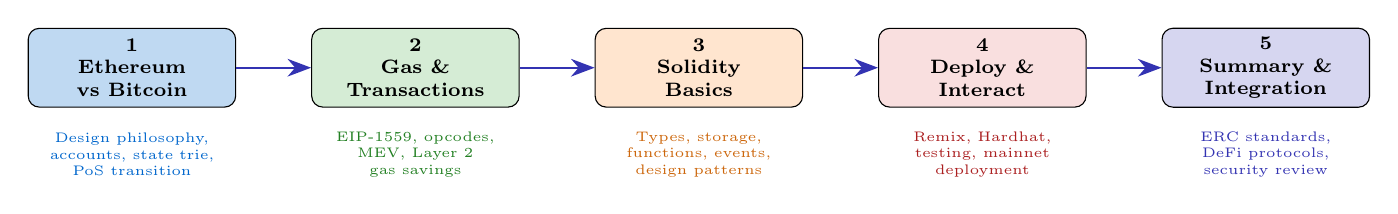
\begin{tikzpicture}[
  rbox/.style={draw,rounded corners=4pt,minimum width=2.6cm,minimum height=1cm,
    font=\scriptsize\bfseries,align=center,text width=2.4cm},
  arr/.style={-{Stealth[length=3mm]},thick,mlpurple}
]
  \node[rbox,fill=mlblue!25] (s1) at (0,0) {1\\Ethereum\\vs Bitcoin};
  \node[rbox,fill=mlgreen!20] (s2) at (3.6,0) {2\\Gas \&\\Transactions};
  \node[rbox,fill=mlorange!20] (s3) at (7.2,0) {3\\Solidity\\Basics};
  \node[rbox,fill=mlred!15] (s4) at (10.8,0) {4\\Deploy \&\\Interact};
  \node[rbox,fill=mlpurple!20] (s5) at (14.4,0) {5\\Summary \&\\Integration};
  \draw[arr] (s1) -- (s2);
  \draw[arr] (s2) -- (s3);
  \draw[arr] (s3) -- (s4);
  \draw[arr] (s4) -- (s5);
  % Annotations below
  \node[font=\tiny,mlblue,align=center,text width=2.4cm] at (0,-1.1) {Design philosophy,\\accounts, state trie,\\PoS transition};
  \node[font=\tiny,mlgreen!80!black,align=center,text width=2.4cm] at (3.6,-1.1) {EIP-1559, opcodes,\\MEV, Layer 2\\gas savings};
  \node[font=\tiny,mlorange!80!black,align=center,text width=2.4cm] at (7.2,-1.1) {Types, storage,\\functions, events,\\design patterns};
  \node[font=\tiny,mlred!80!black,align=center,text width=2.4cm] at (10.8,-1.1) {Remix, Hardhat,\\testing, mainnet\\deployment};
  \node[font=\tiny,mlpurple,align=center,text width=2.4cm] at (14.4,-1.1) {ERC standards,\\DeFi protocols,\\security review};
\end{tikzpicture}
}%
\end{center}
\vspace{2mm}
\begin{columns}
\column{0.48\textwidth}
\begin{block}{Learning Objectives}
\begin{itemize}\small
  \item Contrast Ethereum's account model with Bitcoin's UTXO model
  \item Analyze gas economics and EIP-1559 fee markets
  \item Write, deploy, and test Solidity smart contracts
  \item Evaluate common vulnerabilities and design patterns
\end{itemize}
\end{block}
\column{0.48\textwidth}
\begin{alertblock}{Central Question}
\small How does Ethereum extend blockchain from a payment ledger to a general-purpose decentralized computation platform?
\end{alertblock}
\vspace{2mm}
\begin{block}{Prerequisites}
\begin{itemize}\small
  \item Blockchain fundamentals (hashing, Merkle trees, consensus)
  \item Basic programming experience
  \item Familiarity with Bitcoin transaction model
\end{itemize}
\end{block}
\end{columns}
\bottomnote{5 sections, $\sim$60 frames covering Ethereum architecture, Solidity, deployment, and DeFi integration}
\end{frame}

\begin{frame}{Learning Objectives}
By the end of this lecture, you will be able to:
\begin{enumerate}
\item \textbf{Compare} Ethereum's account model with Bitcoin's UTXO model
\item \textbf{Calculate} gas costs for transactions using the EIP-1559 fee market mechanism
\item \textbf{Implement} basic Solidity contracts with state variables, functions, and modifiers
\item \textbf{Analyze} smart contract security vulnerabilities (reentrancy, overflow, access control)
\item \textbf{Evaluate} upgradeability patterns and their trust implications
\end{enumerate}
\bottomnote{Bloom's taxonomy levels: Remember $\rightarrow$ Understand $\rightarrow$ Apply $\rightarrow$ Analyze $\rightarrow$ Evaluate $\rightarrow$ Create}
\end{frame}

%--- FRAME 3: Bitcoin vs Ethereum: Design Philosophy ---
\begin{frame}{Bitcoin vs Ethereum: Design Philosophy}
\begin{center}
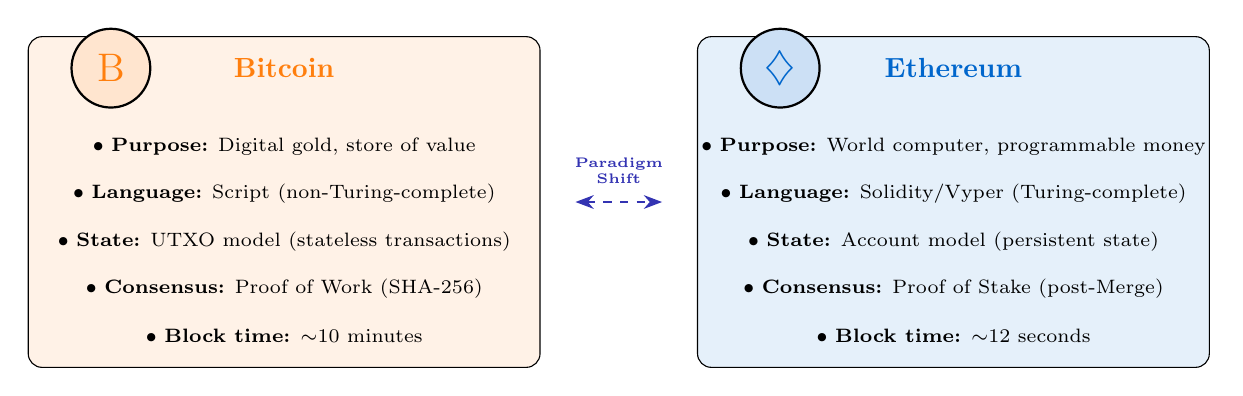
\begin{tikzpicture}[
  card/.style={draw,rounded corners=5pt,minimum width=6.5cm,minimum height=4.2cm,
    font=\small,align=left,text width=6cm},
  icon/.style={draw,circle,minimum size=1cm,font=\Large,thick},
  attr/.style={font=\scriptsize,align=left}
]
  % Bitcoin side
  \node[card,fill=mlorange!10] (btc) at (0,0) {};
  \node[font=\normalsize\bfseries,mlorange] at (0,1.7) {Bitcoin};
  \node[icon,fill=mlorange!20,text=mlorange] at (-2.2,1.7) {B};
  \node[attr] at (0,0.7) {$\bullet$ \textbf{Purpose:} Digital gold, store of value};
  \node[attr] at (0,0.1) {$\bullet$ \textbf{Language:} Script (non-Turing-complete)};
  \node[attr] at (0,-0.5) {$\bullet$ \textbf{State:} UTXO model (stateless transactions)};
  \node[attr] at (0,-1.1) {$\bullet$ \textbf{Consensus:} Proof of Work (SHA-256)};
  \node[attr] at (0,-1.7) {$\bullet$ \textbf{Block time:} $\sim$10 minutes};
  % Ethereum side
  \node[card,fill=mlblue!10] (eth) at (8.5,0) {};
  \node[font=\normalsize\bfseries,mlblue] at (8.5,1.7) {Ethereum};
  \node[icon,fill=mlblue!20,text=mlblue] at (6.3,1.7) {$\diamondsuit$};
  \node[attr] at (8.5,0.7) {$\bullet$ \textbf{Purpose:} World computer, programmable money};
  \node[attr] at (8.5,0.1) {$\bullet$ \textbf{Language:} Solidity/Vyper (Turing-complete)};
  \node[attr] at (8.5,-0.5) {$\bullet$ \textbf{State:} Account model (persistent state)};
  \node[attr] at (8.5,-1.1) {$\bullet$ \textbf{Consensus:} Proof of Stake (post-Merge)};
  \node[attr] at (8.5,-1.7) {$\bullet$ \textbf{Block time:} $\sim$12 seconds};
  % Central comparison arrow
  \draw[{Stealth}-{Stealth},thick,mlpurple,dashed] (3.7,0) -- (4.8,0);
  \node[font=\tiny\bfseries,mlpurple,align=center] at (4.25,0.4) {Paradigm\\Shift};
\end{tikzpicture}
\end{center}
\bottomnote{Vitalik Buterin (2013): ``Bitcoin is a calculator; Ethereum is a smartphone'' -- general-purpose vs.\ single-purpose}
\end{frame}

%--- FRAME 4: Account Model Deep Dive ---
\begin{frame}{Account Model Deep Dive}
\begin{columns}
\column{0.48\textwidth}
\begin{center}
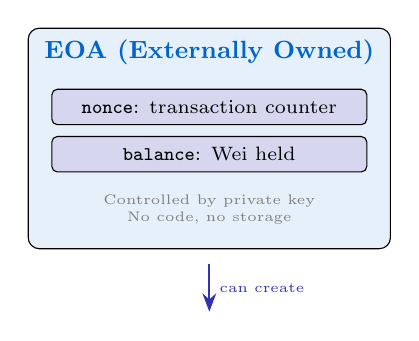
\begin{tikzpicture}[
  acct/.style={draw,rounded corners=4pt,minimum width=4.6cm,minimum height=2.8cm,align=center},
  field/.style={draw,fill=mllavender4,rounded corners=2pt,font=\scriptsize,
    minimum width=4cm,minimum height=0.45cm,align=left}
]
  % EOA
  \node[acct,fill=mlblue!10] (eoa) at (0,0) {};
  \node[font=\small\bfseries,mlblue] at (0,1.1) {EOA (Externally Owned)};
  \node[field] at (0,0.4) {\texttt{nonce}: transaction counter};
  \node[field] at (0,-0.2) {\texttt{balance}: Wei held};
  \node[font=\tiny,mlgray,align=center] at (0,-0.9) {Controlled by private key\\No code, no storage};
  % Arrow between
  \draw[-{Stealth},thick,mlpurple] (0,-1.6) -- (0,-2.2) node[midway,right,font=\tiny]{can create};
\end{tikzpicture}
\end{center}
\column{0.48\textwidth}
\begin{center}
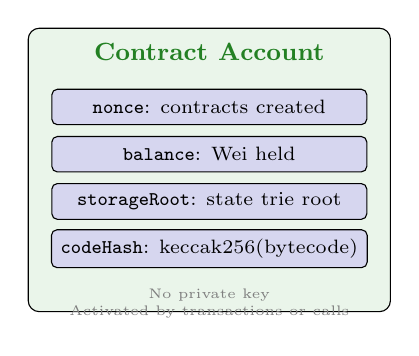
\begin{tikzpicture}[
  acct/.style={draw,rounded corners=4pt,minimum width=4.6cm,minimum height=3.6cm,align=center},
  field/.style={draw,fill=mllavender4,rounded corners=2pt,font=\scriptsize,
    minimum width=4cm,minimum height=0.45cm,align=left}
]
  % Contract Account
  \node[acct,fill=mlgreen!10] (ca) at (0,0) {};
  \node[font=\small\bfseries,mlgreen!80!black] at (0,1.5) {Contract Account};
  \node[field] at (0,0.8) {\texttt{nonce}: contracts created};
  \node[field] at (0,0.2) {\texttt{balance}: Wei held};
  \node[field] at (0,-0.4) {\texttt{storageRoot}: state trie root};
  \node[field] at (0,-1.0) {\texttt{codeHash}: keccak256(bytecode)};
  \node[font=\tiny,mlgray,align=center] at (0,-1.7) {No private key\\Activated by transactions or calls};
\end{tikzpicture}
\end{center}
\end{columns}
\vspace{3mm}
\begin{block}{Key Differences from Bitcoin's UTXO Model}
\begin{itemize}\small
  \item \textbf{UTXO}: Each ``coin'' is a discrete, unspent output consumed entirely -- naturally parallel but stateless
  \item \textbf{Account}: Global state maps addresses to balances/storage -- enables complex state transitions but requires sequential nonce ordering
  \item \textbf{Trade-off}: Account model simplifies smart contract programming at the cost of reduced parallelism
\end{itemize}
\end{block}
\bottomnote{Every Ethereum address is 20 bytes (160 bits) derived from keccak256 of the public key}
\end{frame}

%--- FRAME 5: State Trie Architecture ---
\begin{frame}{State Trie Architecture}
\begin{columns}
\column{0.55\textwidth}
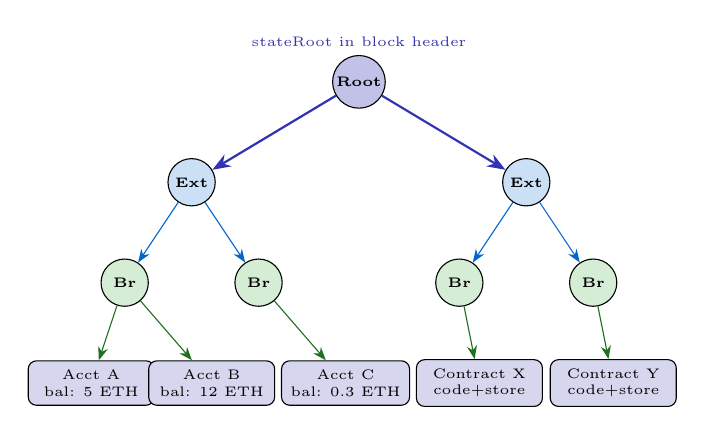
\begin{tikzpicture}[
  trienode/.style={draw,circle,minimum size=0.6cm,font=\tiny\bfseries,inner sep=1pt},
  leafnode/.style={draw,rounded corners=3pt,fill=mllavender4,font=\tiny,
    minimum width=1.6cm,minimum height=0.5cm,align=center},
  scale=0.85
]
  % Root
  \node[trienode,fill=mlpurple!30] (root) at (4,4.5) {Root};
  % Level 1
  \node[trienode,fill=mlblue!20] (n1) at (1.5,3) {Ext};
  \node[trienode,fill=mlblue!20] (n2) at (6.5,3) {Ext};
  % Level 2 - branch
  \node[trienode,fill=mlgreen!20] (b1) at (0.5,1.5) {Br};
  \node[trienode,fill=mlgreen!20] (b2) at (2.5,1.5) {Br};
  \node[trienode,fill=mlgreen!20] (b3) at (5.5,1.5) {Br};
  \node[trienode,fill=mlgreen!20] (b4) at (7.5,1.5) {Br};
  % Leaves
  \node[leafnode] (l1) at (0,0) {Acct A\\bal: 5 ETH};
  \node[leafnode] (l2) at (1.8,0) {Acct B\\bal: 12 ETH};
  \node[leafnode] (l3) at (3.8,0) {Acct C\\bal: 0.3 ETH};
  \node[leafnode] (l4) at (5.8,0) {Contract X\\code+store};
  \node[leafnode] (l5) at (7.8,0) {Contract Y\\code+store};
  % Edges
  \draw[-{Stealth},mlpurple,thick] (root) -- (n1);
  \draw[-{Stealth},mlpurple,thick] (root) -- (n2);
  \draw[-{Stealth},mlblue] (n1) -- (b1);
  \draw[-{Stealth},mlblue] (n1) -- (b2);
  \draw[-{Stealth},mlblue] (n2) -- (b3);
  \draw[-{Stealth},mlblue] (n2) -- (b4);
  \draw[-{Stealth},mlgreen!70!black] (b1) -- (l1);
  \draw[-{Stealth},mlgreen!70!black] (b1) -- (l2);
  \draw[-{Stealth},mlgreen!70!black] (b2) -- (l3);
  \draw[-{Stealth},mlgreen!70!black] (b3) -- (l4);
  \draw[-{Stealth},mlgreen!70!black] (b4) -- (l5);
  % State root label
  \node[font=\tiny,mlpurple,align=center] at (4,5.1) {stateRoot in block header};
\end{tikzpicture}
\column{0.42\textwidth}
\begin{block}{Modified Merkle Patricia Trie}
\begin{itemize}\small
  \item \textbf{3 node types}: Extension, Branch (16 children), Leaf
  \item Keys are nibble paths (hex characters of address)
  \item Path compression via extension nodes
  \item Every state change produces a \textbf{new root hash}
\end{itemize}
\end{block}
\vspace{2mm}
\begin{block}{Four Tries per Block}
\begin{enumerate}\small
  \item \textbf{State trie}: all account data
  \item \textbf{Storage trie}: per-contract storage (nested)
  \item \textbf{Transaction trie}: block transactions
  \item \textbf{Receipt trie}: execution results
\end{enumerate}
\end{block}
\vspace{2mm}
\begin{alertblock}{Proof of Inclusion}
\small Any account state is verifiable with $\mathcal{O}(\log n)$ hashes from the root -- no need to download full state.
\end{alertblock}
\end{columns}
\bottomnote{Ethereum's state trie currently stores $>$250M accounts; each block header commits to the entire world state}
\end{frame}

%--- FRAME 6: Ethereum Block Structure ---
\begin{frame}{Ethereum Block Structure}
\begin{columns}
\column{0.52\textwidth}
\begin{center}
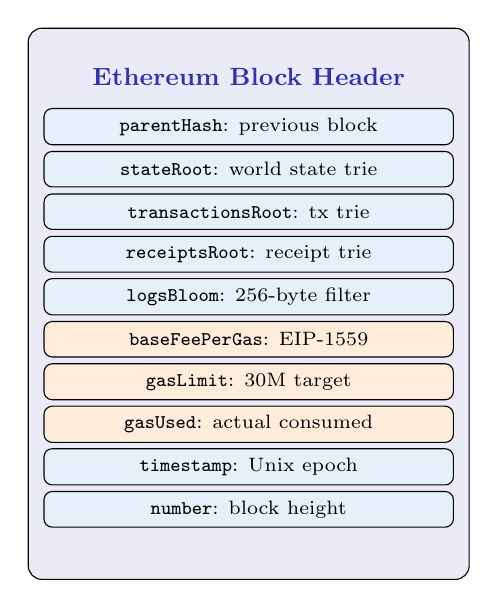
\begin{tikzpicture}[
  hdr/.style={draw,rounded corners=3pt,fill=mlblue!10,font=\scriptsize,
    minimum width=5.2cm,minimum height=0.45cm,align=left},
  scale=0.9
]
  \node[draw,rounded corners=5pt,fill=mlpurple!10,minimum width=5.6cm,minimum height=7cm] (blk) at (0,0) {};
  \node[font=\small\bfseries,mlpurple] at (0,3.2) {Ethereum Block Header};
  \node[hdr] at (0,2.5) {\texttt{parentHash}: previous block};
  \node[hdr] at (0,1.9) {\texttt{stateRoot}: world state trie};
  \node[hdr] at (0,1.3) {\texttt{transactionsRoot}: tx trie};
  \node[hdr] at (0,0.7) {\texttt{receiptsRoot}: receipt trie};
  \node[hdr] at (0,0.1) {\texttt{logsBloom}: 256-byte filter};
  \node[hdr,fill=mlorange!15] at (0,-0.5) {\texttt{baseFeePerGas}: EIP-1559};
  \node[hdr,fill=mlorange!15] at (0,-1.1) {\texttt{gasLimit}: 30M target};
  \node[hdr,fill=mlorange!15] at (0,-1.7) {\texttt{gasUsed}: actual consumed};
  \node[hdr] at (0,-2.3) {\texttt{timestamp}: Unix epoch};
  \node[hdr] at (0,-2.9) {\texttt{number}: block height};
\end{tikzpicture}
\end{center}
\column{0.44\textwidth}
\begin{block}{Bitcoin vs Ethereum Header}
\small
\begin{tabular}{@{}lcc@{}}
\toprule
\textbf{Field} & \textbf{BTC} & \textbf{ETH} \\
\midrule
Parent hash & $\checkmark$ & $\checkmark$ \\
Merkle root & 1 (txs) & 3 tries \\
Nonce/PoW & $\checkmark$ & -- (PoS) \\
State root & -- & $\checkmark$ \\
Gas fields & -- & $\checkmark$ \\
Logs bloom & -- & $\checkmark$ \\
Difficulty & $\checkmark$ & -- (PoS) \\
\bottomrule
\end{tabular}
\end{block}
\vspace{2mm}
\begin{block}{Post-Merge Additions}
\begin{itemize}\small
  \item \texttt{withdrawalsRoot}: validator withdrawals
  \item \texttt{blobGasUsed}: EIP-4844 blobs (Dencun)
  \item \texttt{parentBeaconBlockRoot}: consensus layer link
\end{itemize}
\end{block}
\begin{alertblock}{Key Insight}
\small Ethereum's header commits to the \textbf{entire world state}, not just transactions -- enabling light client state proofs.
\end{alertblock}
\end{columns}
\bottomnote{Ethereum block headers are $\sim$500 bytes vs Bitcoin's 80 bytes -- more data enables richer verification}
\end{frame}

%--- FRAME 7: Transaction Types ---
\begin{frame}{Transaction Types}
\begin{center}
\small
\adjustbox{max width=\textwidth}{%
\begin{tabular}{@{}llll@{}}
\toprule
& \textbf{Type 0 (Legacy)} & \textbf{Type 1 (EIP-2930)} & \textbf{Type 2 (EIP-1559)} \\
\midrule
\textbf{EIP} & Pre-Berlin & EIP-2930 & EIP-1559 \\
\textbf{Fee model} & Single \texttt{gasPrice} & Single \texttt{gasPrice} & \texttt{baseFee} + \texttt{priorityFee} \\
\textbf{Access list} & -- & $\checkmark$ & $\checkmark$ \\
\textbf{Fee burning} & -- & -- & $\checkmark$ (base fee burned) \\
\textbf{Key fields} & \texttt{nonce, to, value,} & + \texttt{accessList} & + \texttt{maxFeePerGas,} \\
& \texttt{gasPrice, gas,} & \texttt{[addr, slots]} & \texttt{maxPriorityFee,} \\
& \texttt{data, v, r, s} & & \texttt{accessList} \\
\textbf{Gas savings} & Baseline & Warm storage discount & Predictable pricing \\
\bottomrule
\end{tabular}
}%
\end{center}
\vspace{2mm}
\begin{columns}
\column{0.48\textwidth}
\begin{block}{Access Lists (Type 1+)}
\begin{itemize}\small
  \item Pre-declare storage slots and addresses you will access
  \item First access to cold slot: 2100 gas $\to$ 100 gas (warm)
  \item Prevents surprise gas costs from \texttt{SLOAD} repricing
\end{itemize}
\end{block}
\column{0.48\textwidth}
\begin{block}{EIP-1559 Advantage (Type 2)}
\begin{itemize}\small
  \item Users set \textbf{max willingness to pay}, not exact price
  \item Base fee auto-adjusts -- no more fee guessing
  \item Overpayment is \textbf{refunded}, not captured by validator
  \item Base fee is burned $\to$ deflationary pressure on ETH
\end{itemize}
\end{block}
\end{columns}
\bottomnote{As of 2024, >95\% of Ethereum transactions use Type 2 (EIP-1559) for predictable fee estimation}
\end{frame}

%--- FRAME 8: EIP-1559 Fee Market ---
\begin{frame}{EIP-1559 Fee Market Mechanism}
\begin{columns}
\column{0.52\textwidth}
\begin{block}{Base Fee Adjustment Formula}
\[
\text{baseFee}_{\text{new}} = \text{baseFee}_{\text{old}} \times \left(1 + \frac{1}{8} \times \frac{\text{gasUsed} - \text{target}}{\text{target}}\right)
\]
\end{block}
\vspace{1mm}
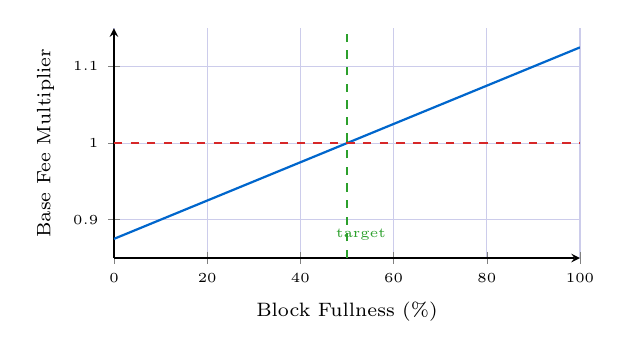
\begin{tikzpicture}
\begin{axis}[
  width=7.5cm, height=4.5cm,
  xlabel={Block Fullness (\%)},
  ylabel={Base Fee Multiplier},
  xlabel style={font=\scriptsize},
  ylabel style={font=\scriptsize},
  tick label style={font=\tiny},
  xmin=0, xmax=100,
  ymin=0.85, ymax=1.15,
  grid=major,
  grid style={mllavender3},
  axis lines=left,
  every axis plot/.append style={thick}
]
\addplot[mlblue,domain=0:100,samples=50] {1 + (1/8)*((x/100*30)-15)/15};
\addplot[mlred,dashed,domain=0:100] {1};
\draw[mlgreen,thick,dashed] (axis cs:50,0.85) -- (axis cs:50,1.15);
\node[font=\tiny,mlgreen] at (axis cs:53,0.88) {target};
\end{axis}
\end{tikzpicture}
\column{0.44\textwidth}
\begin{block}{Mechanism Properties}
\begin{itemize}\small
  \item \textbf{Target}: 15M gas (50\% of 30M limit)
  \item \textbf{Max change}: $\pm$12.5\% per block
  \item Block $<$50\% full $\to$ base fee \textbf{decreases}
  \item Block $>$50\% full $\to$ base fee \textbf{increases}
  \item Empty block: fee drops by 12.5\%
  \item Full block: fee rises by 12.5\%
\end{itemize}
\end{block}
\vspace{2mm}
\begin{block}{User Pays}
\[
\text{fee} = \min(\texttt{maxFee},\;\texttt{baseFee} + \texttt{tip})
\]
\begin{itemize}\small
  \item \texttt{baseFee} $\to$ \textbf{burned} (destroyed)
  \item \texttt{priorityFee} (tip) $\to$ validator
  \item Excess refunded to sender
\end{itemize}
\end{block}
\begin{alertblock}{Deflationary Effect}
\small Since Aug 2021: $>$4M ETH burned. During high activity, burn rate can exceed issuance $\to$ net deflation.
\end{alertblock}
\end{columns}
\bottomnote{EIP-1559 (London upgrade, Aug 2021) fundamentally changed Ethereum's monetary policy by introducing fee burning}
\end{frame}

%--- FRAME 9: The Merge: PoW to PoS ---
\begin{frame}{The Merge: PoW to PoS}
\begin{center}
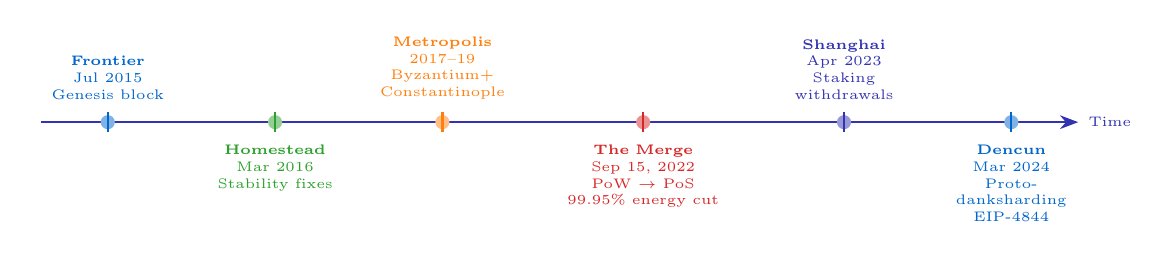
\begin{tikzpicture}[scale=0.85]
  % Timeline
  \draw[-{Stealth},thick,mlpurple] (0,0) -- (15.5,0) node[right,font=\tiny]{Time};
  % Eras
  \foreach \x/\yr/\era/\col in {
    1/2015/Frontier/mlblue,
    3.5/2016/Homestead/mlgreen,
    6/2017-19/Metropolis/mlorange,
    9/Sep 2022/The Merge/mlred,
    12/Apr 2023/Shanghai/mlpurple,
    14.5/Mar 2024/Dencun/mlblue}{
    \fill[\col!50] (\x,0) circle(3pt);
    \draw[\col,thick] (\x,0.15)--(\x,-0.15);
  }
  % Labels above/below alternating
  \node[above,font=\tiny,mlblue,align=center,text width=1.8cm] at (1,0.2) {\textbf{Frontier}\\Jul 2015\\Genesis block};
  \node[below,font=\tiny,mlgreen,align=center,text width=1.8cm] at (3.5,-0.2) {\textbf{Homestead}\\Mar 2016\\Stability fixes};
  \node[above,font=\tiny,mlorange,align=center,text width=2cm] at (6,0.2) {\textbf{Metropolis}\\2017--19\\Byzantium+\\Constantinople};
  \node[below,font=\tiny,mlred,align=center,text width=2cm] at (9,-0.2) {\textbf{The Merge}\\Sep 15, 2022\\PoW $\to$ PoS\\99.95\% energy cut};
  \node[above,font=\tiny,mlpurple,align=center,text width=2cm] at (12,0.2) {\textbf{Shanghai}\\Apr 2023\\Staking\\withdrawals};
  \node[below,font=\tiny,mlblue,align=center,text width=2cm] at (14.5,-0.2) {\textbf{Dencun}\\Mar 2024\\Proto-danksharding\\EIP-4844};
\end{tikzpicture}
\end{center}
\vspace{2mm}
\begin{columns}
\column{0.48\textwidth}
\begin{block}{Before the Merge (PoW)}
\begin{itemize}\small
  \item Miners solve SHA-3/Ethash puzzles
  \item $\sim$15 TH/s network hashrate
  \item Energy: $\sim$78 TWh/year (comparable to Chile)
  \item Block reward: 2 ETH + fees
  \item Issuance: $\sim$13,000 ETH/day
\end{itemize}
\end{block}
\column{0.48\textwidth}
\begin{block}{After the Merge (PoS)}
\begin{itemize}\small
  \item Validators stake 32 ETH as collateral
  \item Randomly selected to propose blocks
  \item Energy: $\sim$0.01 TWh/year (\textbf{99.95\% reduction})
  \item Issuance: $\sim$1,600 ETH/day
  \item Net issuance often \textbf{negative} (deflationary)
\end{itemize}
\end{block}
\end{columns}
\vspace{1mm}
\begin{alertblock}{Technical Achievement}
\small The Merge was the largest live infrastructure migration in crypto history -- swapping consensus on a \$200B+ network with zero downtime.
\end{alertblock}
\bottomnote{Beacon Chain launched Dec 2020; merged with execution layer Sep 15, 2022 at TTD = 58,750,000,000,000,000,000,000}
\end{frame}

%--- FRAME 10: Validator Economics ---
\begin{frame}{Validator Economics}
\begin{columns}
\column{0.52\textwidth}
\begin{center}
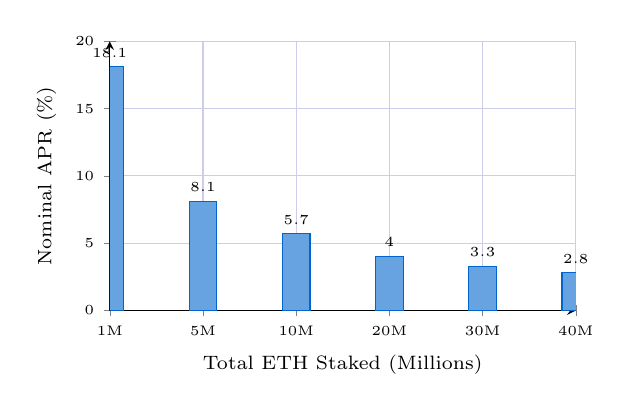
\begin{tikzpicture}
\begin{axis}[
  ybar,
  width=7.5cm, height=5cm,
  xlabel={Total ETH Staked (Millions)},
  ylabel={Nominal APR (\%)},
  xlabel style={font=\scriptsize},
  ylabel style={font=\scriptsize},
  tick label style={font=\tiny},
  symbolic x coords={1M,5M,10M,20M,30M,40M},
  xtick=data,
  ymin=0, ymax=20,
  bar width=10pt,
  nodes near coords,
  nodes near coords style={font=\tiny},
  every node near coord/.append style={above},
  grid=major,
  grid style={mllavender3},
  axis lines=left
]
\addplot[fill=mlblue!60,draw=mlblue] coordinates {
  (1M,18.1) (5M,8.1) (10M,5.7) (20M,4.0) (30M,3.3) (40M,2.8)
};
\end{axis}
\end{tikzpicture}
\end{center}
\column{0.44\textwidth}
\begin{block}{Staking Requirements}
\small
\begin{tabular}{@{}ll@{}}
\toprule
\textbf{Parameter} & \textbf{Value} \\
\midrule
Min stake & 32 ETH \\
Activation queue & $\sim$1--40 days \\
Withdrawal delay & $\sim$1--5 days \\
Max validators & $\sim$1M (soft) \\
Epoch length & 32 slots (6.4 min) \\
Slot time & 12 seconds \\
\bottomrule
\end{tabular}
\end{block}
\vspace{2mm}
\begin{block}{Slashing Conditions}
\begin{itemize}\small
  \item \textbf{Double voting}: proposing 2 blocks in same slot
  \item \textbf{Surround voting}: contradictory attestations
  \item Penalty: 1/32 of stake initially, up to full stake
  \item Correlated slashing: penalty increases if many slash simultaneously
\end{itemize}
\end{block}
\end{columns}
\vspace{1mm}
\begin{alertblock}{Reward Sources}
\small Validators earn from: (1) attestation rewards, (2) block proposal rewards, (3) sync committee duties, (4) MEV tips via mev-boost. Total APR $\approx$ 4--5\% at 30M ETH staked.
\end{alertblock}
\bottomnote{APR follows inverse square root: $\text{APR} \propto 1/\sqrt{\text{total\_staked}}$ -- incentivizes early participation}
\end{frame}

%--- FRAME 11: Ethereum vs Bitcoin Summary Table ---
\begin{frame}{Ethereum vs Bitcoin: Comprehensive Comparison}
\begin{center}
\small
\begin{tabular}{@{}lll@{}}
\toprule
\textbf{Dimension} & \textbf{Bitcoin} & \textbf{Ethereum} \\
\midrule
\textbf{Consensus} & Proof of Work (SHA-256) & Proof of Stake (Casper FFG) \\
\textbf{Block time} & $\sim$10 minutes & $\sim$12 seconds \\
\textbf{Finality} & Probabilistic (6 conf $\approx$ 60 min) & Economic ($\sim$13 min, 2 epochs) \\
\textbf{State model} & UTXO (stateless) & Account (stateful) \\
\textbf{Smart contracts} & Limited (Script) & Turing-complete (EVM) \\
\textbf{Programming} & Script (stack-based, $\sim$100 opcodes) & Solidity/Vyper ($\sim$140 opcodes) \\
\textbf{Supply cap} & 21M BTC (hard cap) & No hard cap (net issuance $\approx$ 0) \\
\textbf{Fee model} & Fee market auction & EIP-1559 (base + tip, burning) \\
\textbf{Throughput} & $\sim$7 TPS & $\sim$15--30 TPS (L1) \\
\textbf{Energy use} & $\sim$150 TWh/yr & $\sim$0.01 TWh/yr \\
\textbf{Native token} & BTC (divisible to satoshi) & ETH (divisible to Wei, $10^{-18}$) \\
\textbf{Upgrades} & BIPs, conservative & EIPs, more frequent forks \\
\textbf{L2 scaling} & Lightning Network (channels) & Rollups (Optimistic, ZK) \\
\textbf{Primary use} & Store of value, payments & DeFi, NFTs, DAOs, dApps \\
\bottomrule
\end{tabular}
\end{center}
\vspace{2mm}
\begin{alertblock}{Key Takeaway}
\small Bitcoin optimizes for \textbf{security and simplicity} (sound money); Ethereum optimizes for \textbf{expressiveness and composability} (programmable finance). They serve complementary roles in the ecosystem.
\end{alertblock}
\bottomnote{Both networks have >99.9\% uptime since launch -- a remarkable achievement for decentralized systems}
\end{frame}

\section{Gas and Transactions}

%--- FRAME 12: Gas: The Execution Fuel ---
\begin{frame}{Gas: The Execution Fuel}
\begin{columns}
\column{0.48\textwidth}
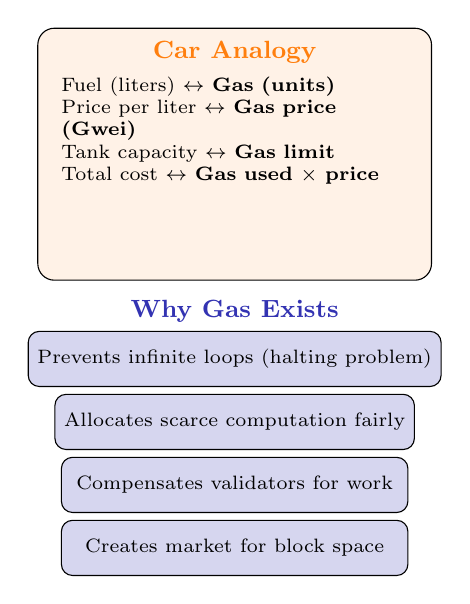
\begin{tikzpicture}[
  box/.style={draw,rounded corners=4pt,fill=mllavender4,font=\scriptsize,
    minimum width=4.4cm,minimum height=0.7cm,align=center}
]
  % Fuel gauge analogy
  \node[draw,rounded corners=6pt,fill=mlorange!10,minimum width=5cm,minimum height=3.2cm] at (0,2.5) {};
  \node[font=\small\bfseries,mlorange] at (0,3.8) {Car Analogy};
  \node[font=\scriptsize,align=left,text width=4.4cm] at (0,2.8) {
    Fuel (liters) $\leftrightarrow$ \textbf{Gas (units)}\\
    Price per liter $\leftrightarrow$ \textbf{Gas price (Gwei)}\\
    Tank capacity $\leftrightarrow$ \textbf{Gas limit}\\
    Total cost $\leftrightarrow$ \textbf{Gas used $\times$ price}
  };
  % Why gas exists
  \node[font=\small\bfseries,mlpurple] at (0,0.5) {Why Gas Exists};
  \node[box] at (0,-0.1) {Prevents infinite loops (halting problem)};
  \node[box] at (0,-0.9) {Allocates scarce computation fairly};
  \node[box] at (0,-1.7) {Compensates validators for work};
  \node[box] at (0,-2.5) {Creates market for block space};
\end{tikzpicture}
\column{0.48\textwidth}
\begin{block}{Gas Mechanics}
\begin{itemize}\small
  \item Every EVM opcode has a fixed gas cost
  \item Transaction specifies a \texttt{gasLimit} (max gas to use)
  \item If execution exceeds limit $\to$ \textbf{revert} (state unchanged)
  \item Unused gas is \textbf{refunded} to sender
  \item Gas is \textbf{not} a token -- it is denominated in ETH
\end{itemize}
\end{block}
\vspace{2mm}
\begin{block}{Units}
\small
\begin{tabular}{@{}lrl@{}}
\toprule
\textbf{Unit} & \textbf{Wei} & \textbf{Use} \\
\midrule
Wei & 1 & Smallest unit \\
Gwei & $10^{9}$ & Gas prices \\
Ether & $10^{18}$ & Account balance \\
\bottomrule
\end{tabular}
\end{block}
\vspace{2mm}
\begin{alertblock}{Turing Tax}
\small Gas is the ``Turing tax'' -- the cost of arbitrary computation on a replicated state machine. Every node re-executes every transaction.
\end{alertblock}
\end{columns}
\bottomnote{A simple ETH transfer costs exactly 21,000 gas; a Uniswap swap costs $\sim$150,000 gas}
\end{frame}

%--- FRAME 13: Gas Cost Table ---
\begin{frame}{EVM Opcode Gas Costs}
\begin{columns}
\column{0.48\textwidth}
\begin{center}
\small
\begin{tabular}{@{}llr@{}}
\toprule
\textbf{Category} & \textbf{Opcode} & \textbf{Gas} \\
\midrule
\rowcolor{mlblue!10}
\multicolumn{3}{@{}l}{\textbf{\textcolor{mlblue}{Arithmetic}}} \\
& ADD / SUB & 3 \\
& MUL / DIV & 5 \\
& ADDMOD / MULMOD & 8 \\
& EXP & 10+ \\
\rowcolor{mlgreen!10}
\multicolumn{3}{@{}l}{\textbf{\textcolor{mlgreen!80!black}{Hashing}}} \\
& KECCAK256 (base) & 30 \\
& + per word & 6 \\
\rowcolor{mlorange!10}
\multicolumn{3}{@{}l}{\textbf{\textcolor{mlorange}{Memory}}} \\
& MLOAD / MSTORE & 3 \\
& MSTORE8 & 3 \\
\bottomrule
\end{tabular}
\end{center}
\column{0.48\textwidth}
\begin{center}
\small
\begin{tabular}{@{}llr@{}}
\toprule
\textbf{Category} & \textbf{Opcode} & \textbf{Gas} \\
\midrule
\rowcolor{mlred!10}
\multicolumn{3}{@{}l}{\textbf{\textcolor{mlred}{Storage (most expensive)}}} \\
& SLOAD (cold) & 2,100 \\
& SLOAD (warm) & 100 \\
& SSTORE (new) & 20,000 \\
& SSTORE (update) & 5,000 \\
\rowcolor{mlpurple!10}
\multicolumn{3}{@{}l}{\textbf{\textcolor{mlpurple}{Contract Creation}}} \\
& CREATE & 32,000 \\
& CREATE2 & 32,000 \\
\rowcolor{mlgray!10}
\multicolumn{3}{@{}l}{\textbf{\textcolor{mlgray}{Calls}}} \\
& CALL (cold) & 2,600 \\
& CALL (warm) & 100 \\
& DELEGATECALL & 2,600 \\
\bottomrule
\end{tabular}
\end{center}
\end{columns}
\vspace{2mm}
\begin{alertblock}{Key Insight: Storage Dominates Cost}
\small Storage operations are 100--6,600$\times$ more expensive than arithmetic. A single \texttt{SSTORE} to a new slot (20,000 gas) costs as much as 6,667 additions. \textbf{Optimizing storage access is the primary lever for gas reduction.}
\end{alertblock}
\bottomnote{Gas costs were recalibrated in EIP-2929 (Berlin, Apr 2021) introducing cold/warm access pricing}
\end{frame}

%--- FRAME 14: Gas Limit & Block Space ---
\begin{frame}{Gas Limit \& Block Space}
\begin{columns}
\column{0.52\textwidth}
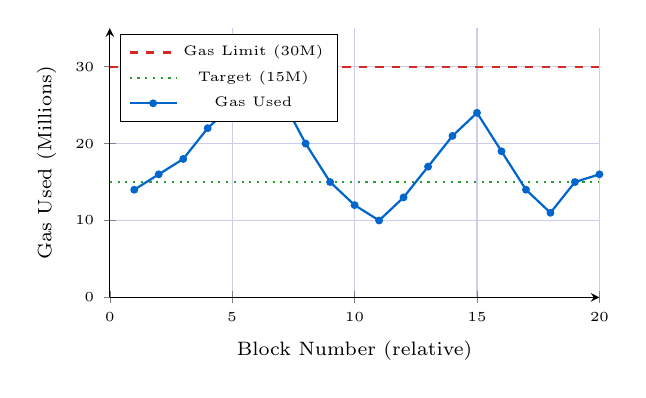
\begin{tikzpicture}
\begin{axis}[
  width=7.8cm, height=5cm,
  xlabel={Block Number (relative)},
  ylabel={Gas Used (Millions)},
  xlabel style={font=\scriptsize},
  ylabel style={font=\scriptsize},
  tick label style={font=\tiny},
  xmin=0, xmax=20,
  ymin=0, ymax=35,
  grid=major,
  grid style={mllavender3},
  axis lines=left,
  legend style={font=\tiny,at={(0.02,0.98)},anchor=north west}
]
% Gas limit line
\addplot[mlred,thick,dashed,domain=0:20] {30};
\addlegendentry{Gas Limit (30M)}
% Target line
\addplot[mlgreen,thick,dotted,domain=0:20] {15};
\addlegendentry{Target (15M)}
% Simulated gas usage
\addplot[mlblue,thick,mark=*,mark size=1pt] coordinates {
  (1,14) (2,16) (3,18) (4,22) (5,25) (6,28) (7,26) (8,20)
  (9,15) (10,12) (11,10) (12,13) (13,17) (14,21) (15,24)
  (16,19) (17,14) (18,11) (19,15) (20,16)
};
\addlegendentry{Gas Used}
% Shaded target zone
\addplot[mlgreen!20,fill opacity=0.3,draw=none] coordinates {
  (0,13) (20,13) (20,17) (0,17)
} \closedcycle;
\end{axis}
\end{tikzpicture}
\column{0.44\textwidth}
\begin{block}{Block Space Economics}
\begin{itemize}\small
  \item \textbf{Gas limit}: 30M gas (hard ceiling)
  \item \textbf{Target}: 15M gas (50\% of limit)
  \item Blocks can temporarily burst to 2$\times$ target
  \item EIP-1559 adjusts base fee to converge on target
\end{itemize}
\end{block}
\vspace{2mm}
\begin{block}{What Fits in a Block?}
\small
\begin{tabular}{@{}lr@{}}
\toprule
\textbf{Operation} & \textbf{Max/Block} \\
\midrule
ETH transfers & $\sim$1,428 \\
ERC-20 transfers & $\sim$460 \\
Uniswap swaps & $\sim$200 \\
NFT mints & $\sim$120 \\
Contract deploys & $\sim$5--15 \\
\bottomrule
\end{tabular}
\end{block}
\vspace{1mm}
\begin{alertblock}{Elasticity}
\small The 2$\times$ buffer absorbs demand spikes while the fee mechanism ensures long-run convergence to 50\% utilization.
\end{alertblock}
\end{columns}
\bottomnote{Block space is Ethereum's scarce resource -- every 12 seconds, validators auction $\sim$30M gas units}
\end{frame}

%--- FRAME 15: EIP-1559 Deep Dive ---
\begin{frame}{EIP-1559 Deep Dive: Fee Flow}
\begin{center}
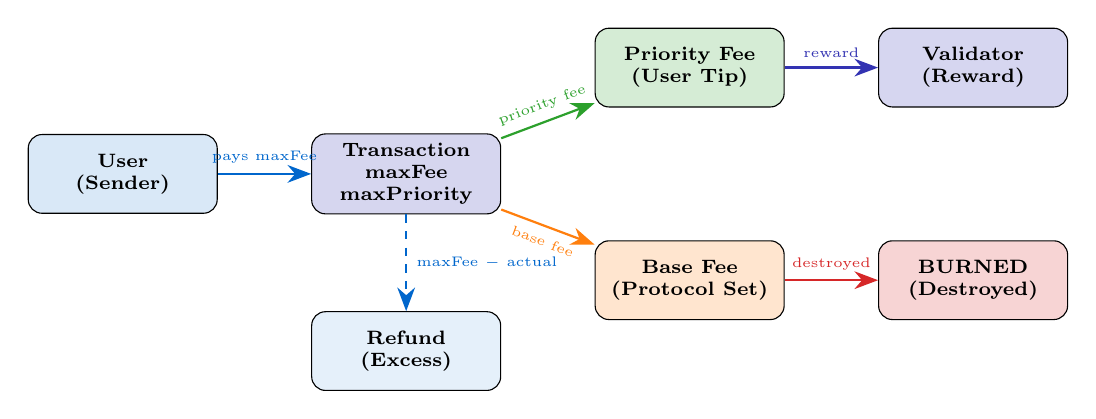
\begin{tikzpicture}[
  box/.style={draw,rounded corners=5pt,minimum width=2.4cm,minimum height=1cm,
    font=\scriptsize\bfseries,align=center},
  arr/.style={-{Stealth[length=3mm]},thick},
  scale=0.9
]
  % User
  \node[box,fill=mlblue!15] (user) at (0,0) {User\\(Sender)};
  % Transaction
  \node[box,fill=mllavender4] (tx) at (4,0) {Transaction\\maxFee\\maxPriority};
  % Split
  \node[box,fill=mlorange!20] (base) at (8,-1.5) {Base Fee\\(Protocol Set)};
  \node[box,fill=mlgreen!20] (tip) at (8,1.5) {Priority Fee\\(User Tip)};
  % Destinations
  \node[box,fill=mlred!20] (burn) at (12,-1.5) {BURNED\\(Destroyed)};
  \node[box,fill=mlpurple!20] (val) at (12,1.5) {Validator\\(Reward)};
  % Refund
  \node[box,fill=mlblue!10] (refund) at (4,-2.5) {Refund\\(Excess)};
  % Arrows
  \draw[arr,mlblue] (user) -- (tx) node[midway,above,font=\tiny]{pays maxFee};
  \draw[arr,mlorange] (tx) -- (base) node[midway,below,font=\tiny,sloped]{base fee};
  \draw[arr,mlgreen] (tx) -- (tip) node[midway,above,font=\tiny,sloped]{priority fee};
  \draw[arr,mlred] (base) -- (burn) node[midway,above,font=\tiny]{destroyed};
  \draw[arr,mlpurple] (tip) -- (val) node[midway,above,font=\tiny]{reward};
  \draw[arr,mlblue,dashed] (tx) -- (refund) node[midway,right,font=\tiny]{maxFee $-$ actual};
\end{tikzpicture}
\end{center}
\vspace{2mm}
\begin{columns}
\column{0.48\textwidth}
\begin{block}{Actual Fee Calculation}
\small
\begin{align*}
\text{effectiveGasPrice} &= \min\!\big(\texttt{maxFee},\\
&\quad \texttt{baseFee} + \texttt{maxPriority}\big) \\
\text{totalFee} &= \text{gasUsed} \times \text{effectiveGasPrice} \\
\text{refund} &= (\texttt{maxFee} - \text{effectiveGasPrice}) \times \text{gasUsed}
\end{align*}
\end{block}
\column{0.48\textwidth}
\begin{block}{Worked Example}
\small
\begin{tabular}{@{}ll@{}}
\texttt{maxFeePerGas} & 50 Gwei \\
\texttt{maxPriorityFee} & 2 Gwei \\
Current \texttt{baseFee} & 30 Gwei \\
\texttt{gasUsed} & 21,000 \\
\midrule
Effective price & $\min(50, 30+2) = 32$ Gwei \\
Total fee & $21{,}000 \times 32 = 672{,}000$ Gwei \\
Burned & $21{,}000 \times 30 = 630{,}000$ Gwei \\
Validator tip & $21{,}000 \times 2 = 42{,}000$ Gwei \\
\end{tabular}
\end{block}
\end{columns}
\bottomnote{The burning mechanism creates a feedback loop: high demand burns more ETH, reducing supply, increasing scarcity}
\end{frame}

%--- FRAME 16: Transaction Lifecycle ---
\begin{frame}{Transaction Lifecycle}
\begin{center}
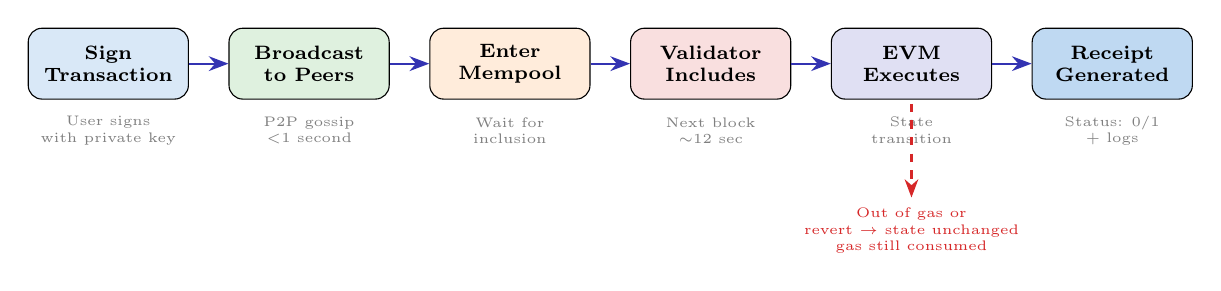
\begin{tikzpicture}[
  procstep/.style={draw,rounded corners=5pt,minimum width=2cm,minimum height=0.9cm,
    font=\scriptsize\bfseries,align=center,text width=1.8cm},
  arr/.style={-{Stealth[length=2.5mm]},thick,mlpurple},
  timing/.style={font=\tiny,mlgray,align=center},
  scale=0.85
]
  % Steps
  \node[procstep,fill=mlblue!15] (s1) at (0,0) {Sign\\Transaction};
  \node[procstep,fill=mlgreen!15] (s2) at (3,0) {Broadcast\\to Peers};
  \node[procstep,fill=mlorange!15] (s3) at (6,0) {Enter\\Mempool};
  \node[procstep,fill=mlred!15] (s4) at (9,0) {Validator\\Includes};
  \node[procstep,fill=mlpurple!15] (s5) at (12,0) {EVM\\Executes};
  \node[procstep,fill=mlblue!25] (s6) at (15,0) {Receipt\\Generated};
  % Arrows
  \draw[arr] (s1) -- (s2);
  \draw[arr] (s2) -- (s3);
  \draw[arr] (s3) -- (s4);
  \draw[arr] (s4) -- (s5);
  \draw[arr] (s5) -- (s6);
  % Timing labels
  \node[timing] at (0,-1) {User signs\\with private key};
  \node[timing] at (3,-1) {P2P gossip\\$<$1 second};
  \node[timing] at (6,-1) {Wait for\\inclusion};
  \node[timing] at (9,-1) {Next block\\$\sim$12 sec};
  \node[timing] at (12,-1) {State\\transition};
  \node[timing] at (15,-1) {Status: 0/1\\+ logs};
  % Failure path
  \draw[-{Stealth},mlred,dashed,thick] (12,-0.6) -- (12,-2) node[below,font=\tiny,mlred,align=center]{Out of gas or\\revert $\to$ state unchanged\\gas still consumed};
\end{tikzpicture}
\end{center}
\vspace{3mm}
\begin{columns}
\column{0.48\textwidth}
\begin{block}{Mempool Dynamics}
\begin{itemize}\small
  \item Transactions ordered by \texttt{effectiveGasPrice} (highest first)
  \item Same-sender txs ordered by \texttt{nonce} (sequential)
  \item Stuck tx: low fee $\to$ replace with higher-fee tx (same nonce)
  \item Mempool is \textbf{not} consensus-critical -- each node has its own
\end{itemize}
\end{block}
\column{0.48\textwidth}
\begin{block}{Finality Timeline}
\begin{itemize}\small
  \item \textbf{Included}: 12 seconds (1 slot)
  \item \textbf{Safe}: $\sim$6.4 minutes (1 epoch, 32 slots)
  \item \textbf{Finalized}: $\sim$13 minutes (2 epochs)
  \item After finalization: reverting requires $\geq$1/3 of all staked ETH to be slashed
\end{itemize}
\end{block}
\end{columns}
\bottomnote{Ethereum processes $\sim$1M transactions/day across 7,200 blocks (12-second slots)}
\end{frame}

%--- FRAME 17: Transaction Receipt & Logs ---
\begin{frame}{Transaction Receipt \& Logs}
\begin{columns}
\column{0.48\textwidth}
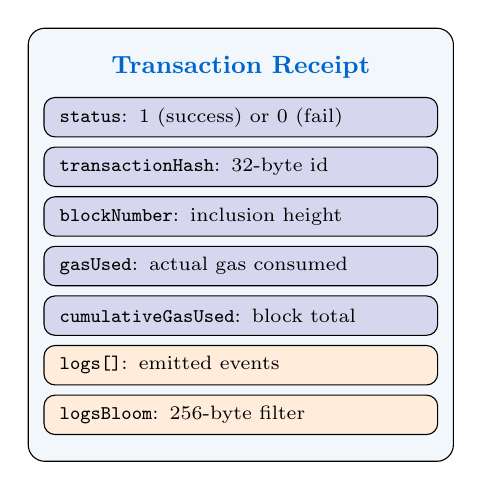
\begin{tikzpicture}[
  rbox/.style={draw,rounded corners=4pt,font=\scriptsize,align=left,
    minimum width=5cm,minimum height=0.5cm,text width=4.6cm},
  scale=0.9
]
  % Receipt container
  \node[draw,rounded corners=6pt,fill=mlblue!5,minimum width=5.4cm,minimum height=5.5cm] at (0,0) {};
  \node[font=\small\bfseries,mlblue] at (0,2.5) {Transaction Receipt};
  \node[rbox,fill=mllavender4] at (0,1.8) {\texttt{status}: 1 (success) or 0 (fail)};
  \node[rbox,fill=mllavender4] at (0,1.1) {\texttt{transactionHash}: 32-byte id};
  \node[rbox,fill=mllavender4] at (0,0.4) {\texttt{blockNumber}: inclusion height};
  \node[rbox,fill=mllavender4] at (0,-0.3) {\texttt{gasUsed}: actual gas consumed};
  \node[rbox,fill=mllavender4] at (0,-1.0) {\texttt{cumulativeGasUsed}: block total};
  \node[rbox,fill=mlorange!15] at (0,-1.7) {\texttt{logs[]}: emitted events};
  \node[rbox,fill=mlorange!15] at (0,-2.4) {\texttt{logsBloom}: 256-byte filter};
\end{tikzpicture}
\column{0.48\textwidth}
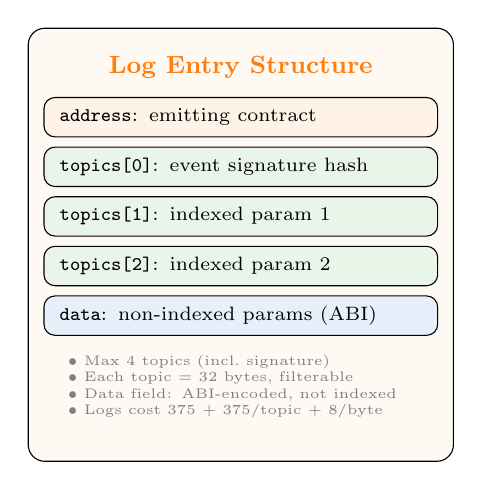
\begin{tikzpicture}[
  lbox/.style={draw,rounded corners=4pt,font=\scriptsize,align=left,
    minimum width=5cm,minimum height=0.5cm,text width=4.6cm},
  scale=0.9
]
  % Log entry
  \node[draw,rounded corners=6pt,fill=mlorange!5,minimum width=5.4cm,minimum height=5.5cm] at (0,0) {};
  \node[font=\small\bfseries,mlorange] at (0,2.5) {Log Entry Structure};
  \node[lbox,fill=mlorange!10] at (0,1.8) {\texttt{address}: emitting contract};
  \node[lbox,fill=mlgreen!10] at (0,1.1) {\texttt{topics[0]}: event signature hash};
  \node[lbox,fill=mlgreen!10] at (0,0.4) {\texttt{topics[1]}: indexed param 1};
  \node[lbox,fill=mlgreen!10] at (0,-0.3) {\texttt{topics[2]}: indexed param 2};
  \node[lbox,fill=mlblue!10] at (0,-1.0) {\texttt{data}: non-indexed params (ABI)};
  % Annotation
  \node[font=\tiny,mlgray,align=left,text width=4.4cm] at (0,-2.0) {
    $\bullet$ Max 4 topics (incl.\ signature)\\
    $\bullet$ Each topic = 32 bytes, filterable\\
    $\bullet$ Data field: ABI-encoded, not indexed\\
    $\bullet$ Logs cost 375 + 375/topic + 8/byte
  };
\end{tikzpicture}
\end{columns}
\vspace{2mm}
\begin{alertblock}{Why Events Matter}
\small Events are 5--100$\times$ cheaper than storage for recording historical data. DApps use \texttt{eth\_getLogs} to reconstruct state from event history. The Bloom filter in each block header enables efficient log scanning.
\end{alertblock}
\bottomnote{Topic[0] = keccak256(``Transfer(address,address,uint256)'') for ERC-20 Transfer events}
\end{frame}

%--- FRAME 18: Estimating Gas Costs ---
\begin{frame}{Estimating Gas Costs: Worked Example}
\begin{columns}
\column{0.48\textwidth}
\begin{block}{Cost Formula}
\[
\text{Cost (ETH)} = \text{gasUsed} \times \text{effectiveGasPrice}
\]
\[
\text{Cost (USD)} = \text{Cost (ETH)} \times \text{ETH/USD price}
\]
\end{block}
\vspace{1mm}
\begin{block}{Unit Conversions}
\small
\begin{tabular}{@{}lcl@{}}
\toprule
\textbf{From} & & \textbf{To} \\
\midrule
1 Gwei & $=$ & $10^{9}$ Wei \\
1 ETH & $=$ & $10^{9}$ Gwei \\
1 ETH & $=$ & $10^{18}$ Wei \\
\bottomrule
\end{tabular}
\end{block}
\vspace{2mm}
\begin{alertblock}{Worked Example: ETH Transfer}
\small
\begin{tabular}{@{}ll@{}}
Gas used & 21,000 \\
Gas price & 30 Gwei \\
Cost (Wei) & $21{,}000 \times 30 \times 10^9$ \\
Cost (ETH) & $0.00063$ ETH \\
ETH price & \$3,000 \\
\textbf{Cost (USD)} & \textbf{\$1.89} \\
\end{tabular}
\end{alertblock}
\column{0.48\textwidth}
\begin{block}{Common Operation Costs (at 30 Gwei)}
\small
\begin{tabular}{@{}lrr@{}}
\toprule
\textbf{Operation} & \textbf{Gas} & \textbf{USD} \\
\midrule
ETH transfer & 21,000 & \$1.89 \\
ERC-20 transfer & 65,000 & \$5.85 \\
ERC-20 approve & 46,000 & \$4.14 \\
Uniswap V3 swap & 150,000 & \$13.50 \\
NFT mint (ERC-721) & 120,000 & \$10.80 \\
Contract deploy & 500,000+ & \$45+ \\
Aave borrow & 350,000 & \$31.50 \\
\bottomrule
\end{tabular}
\end{block}
\vspace{2mm}
\begin{block}{Gas Price History}
\begin{itemize}\small
  \item 2021 bull market: 100--500 Gwei (NFT minting wars)
  \item 2022--23 bear market: 5--20 Gwei
  \item 2024 with L2 adoption: 10--40 Gwei typical
  \item During MEV events: spikes to 1000+ Gwei
\end{itemize}
\end{block}
\end{columns}
\bottomnote{Pro tip: use \texttt{eth\_estimateGas} RPC call before sending -- actual gas may differ from estimates by 10--20\%}
\end{frame}

%--- FRAME 19: Gas Optimization Patterns ---
\begin{frame}{Gas Optimization Patterns}
\begin{center}
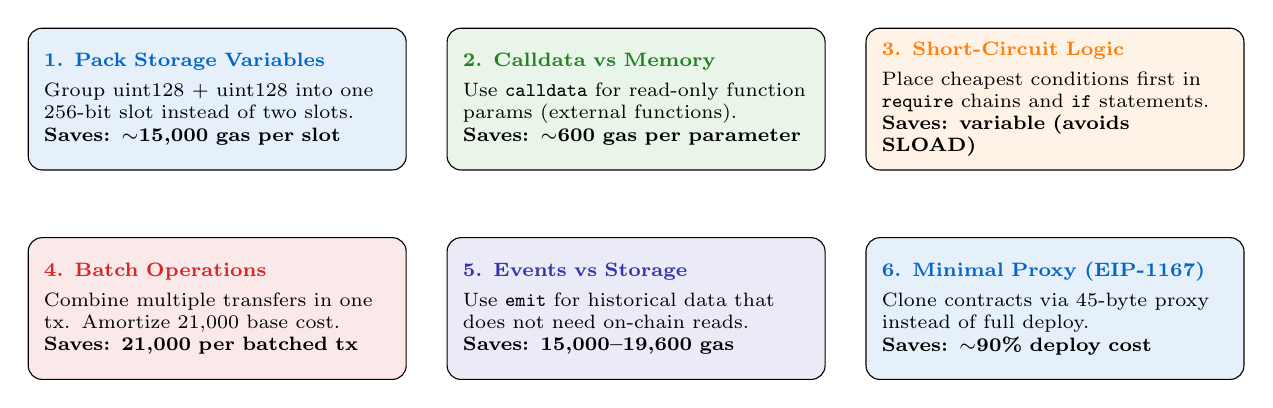
\begin{tikzpicture}[
  card/.style={draw,rounded corners=5pt,minimum width=4.8cm,minimum height=1.8cm,
    font=\scriptsize,align=left,text width=4.4cm},
  scale=0.95
]
  % Row 1
  \node[card,fill=mlblue!10] (c1) at (0,2.2) {
    \textbf{\textcolor{mlblue}{1. Pack Storage Variables}}\\[1mm]
    Group uint128 + uint128 into one 256-bit slot instead of two slots.\\
    \textbf{Saves: $\sim$15,000 gas per slot}
  };
  \node[card,fill=mlgreen!10] (c2) at (5.6,2.2) {
    \textbf{\textcolor{mlgreen!80!black}{2. Calldata vs Memory}}\\[1mm]
    Use \texttt{calldata} for read-only function params (external functions).\\
    \textbf{Saves: $\sim$600 gas per parameter}
  };
  \node[card,fill=mlorange!10] (c3) at (11.2,2.2) {
    \textbf{\textcolor{mlorange}{3. Short-Circuit Logic}}\\[1mm]
    Place cheapest conditions first in \texttt{require} chains and \texttt{if} statements.\\
    \textbf{Saves: variable (avoids SLOAD)}
  };
  % Row 2
  \node[card,fill=mlred!10] (c4) at (0,-0.6) {
    \textbf{\textcolor{mlred}{4. Batch Operations}}\\[1mm]
    Combine multiple transfers in one tx. Amortize 21,000 base cost.\\
    \textbf{Saves: 21,000 per batched tx}
  };
  \node[card,fill=mlpurple!10] (c5) at (5.6,-0.6) {
    \textbf{\textcolor{mlpurple}{5. Events vs Storage}}\\[1mm]
    Use \texttt{emit} for historical data that does not need on-chain reads.\\
    \textbf{Saves: 15,000--19,600 gas}
  };
  \node[card,fill=mlblue!10] (c6) at (11.2,-0.6) {
    \textbf{\textcolor{mlblue}{6. Minimal Proxy (EIP-1167)}}\\[1mm]
    Clone contracts via 45-byte proxy instead of full deploy.\\
    \textbf{Saves: $\sim$90\% deploy cost}
  };
\end{tikzpicture}
\end{center}
\vspace{2mm}
\begin{alertblock}{Rule of Thumb}
\small Optimize storage first (SSTORE/SLOAD dominate costs), then reduce calldata size, then optimize computation. A single unnecessary \texttt{SSTORE} to a new slot costs more than 6,000 arithmetic operations.
\end{alertblock}
\bottomnote{Advanced: Solidity 0.8.19+ supports custom errors (\texttt{error InsufficientBalance()}) saving $\sim$3,000 gas vs string reverts}
\end{frame}

%--- FRAME 20: MEV: Maximal Extractable Value ---
\begin{frame}{MEV: Maximal Extractable Value}
\begin{center}
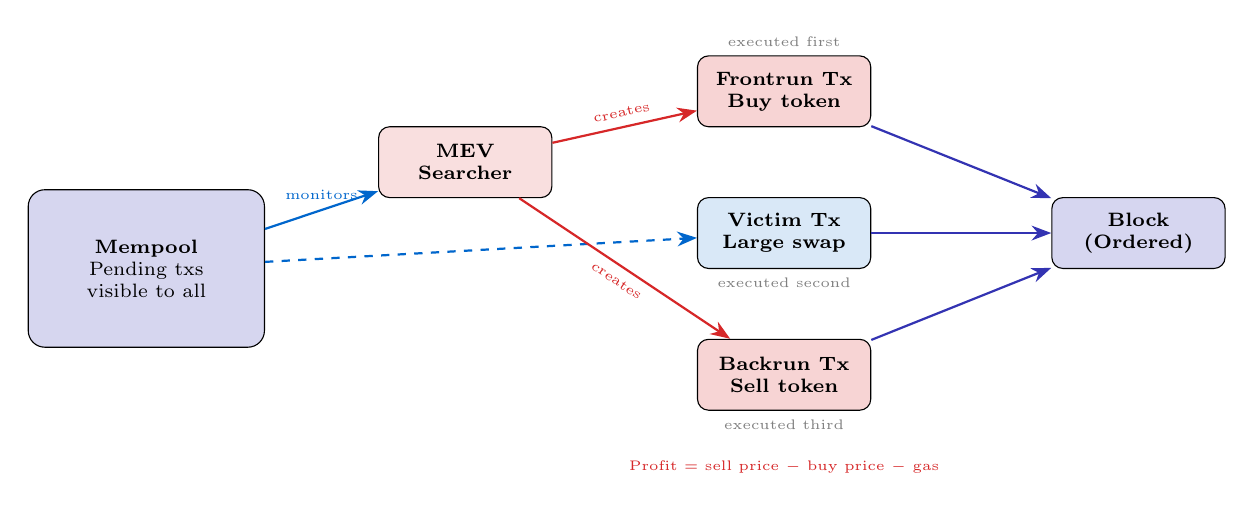
\begin{tikzpicture}[
  box/.style={draw,rounded corners=4pt,minimum width=2.2cm,minimum height=0.9cm,
    font=\scriptsize\bfseries,align=center},
  arr/.style={-{Stealth[length=2.5mm]},thick},
  scale=0.9
]
  % Mempool
  \node[draw,rounded corners=6pt,fill=mllavender4,minimum width=3cm,minimum height=2cm,
    font=\scriptsize,align=center] (pool) at (0,0) {\textbf{Mempool}\\Pending txs\\visible to all};
  % Searcher
  \node[box,fill=mlred!15] (search) at (4.5,1.5) {MEV\\Searcher};
  % Sandwich components
  \node[box,fill=mlred!20] (front) at (9,2.5) {Frontrun Tx\\Buy token};
  \node[box,fill=mlblue!15] (victim) at (9,0.5) {Victim Tx\\Large swap};
  \node[box,fill=mlred!20] (back) at (9,-1.5) {Backrun Tx\\Sell token};
  % Validator
  \node[box,fill=mlpurple!20] (val) at (14,0.5) {Block\\(Ordered)};
  % Arrows
  \draw[arr,mlblue] (pool) -- (search) node[midway,above,font=\tiny]{monitors};
  \draw[arr,mlred] (search) -- (front) node[midway,above,font=\tiny,sloped]{creates};
  \draw[arr,mlblue,dashed] (pool) -- (victim);
  \draw[arr,mlred] (search) -- (back) node[midway,below,font=\tiny,sloped]{creates};
  % To block
  \draw[arr,mlpurple] (front) -- (val);
  \draw[arr,mlpurple] (victim) -- (val);
  \draw[arr,mlpurple] (back) -- (val);
  % Profit annotation
  \node[font=\tiny,mlred,align=center] at (9,-2.8) {Profit = sell price $-$ buy price $-$ gas};
  % Labels
  \node[font=\tiny,mlgray] at (9,3.2) {executed first};
  \node[font=\tiny,mlgray] at (9,-0.2) {executed second};
  \node[font=\tiny,mlgray] at (9,-2.2) {executed third};
\end{tikzpicture}
\end{center}
\vspace{1mm}
\begin{columns}
\column{0.48\textwidth}
\begin{block}{MEV Categories}
\begin{itemize}\small
  \item \textbf{Sandwich attacks}: front + backrun swaps
  \item \textbf{Arbitrage}: price differences across DEXes
  \item \textbf{Liquidations}: seize undercollateralized positions
  \item \textbf{Just-in-time liquidity}: provide LP for single tx
\end{itemize}
\end{block}
\column{0.48\textwidth}
\begin{block}{MEV Mitigation}
\begin{itemize}\small
  \item \textbf{Flashbots Protect}: private tx submission
  \item \textbf{MEV-Boost}: separate block building from proposing
  \item \textbf{Encrypted mempools}: hide tx content until ordering
  \item Cumulative MEV extracted: $>$\$600M (2020--2024)
\end{itemize}
\end{block}
\end{columns}
\bottomnote{MEV is the ``invisible tax'' on DeFi users -- understanding it is crucial for protocol design and user protection}
\end{frame}

%--- FRAME 21: Layer 2 Gas Savings ---
\begin{frame}{Layer 2 Gas Savings}
\begin{columns}
\column{0.55\textwidth}
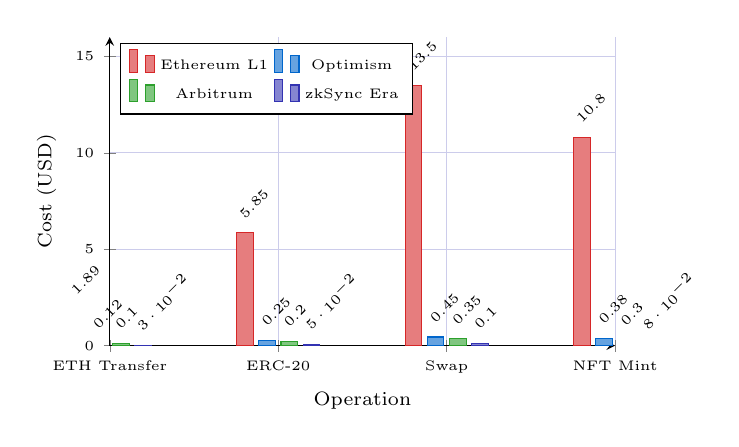
\begin{tikzpicture}
\begin{axis}[
  ybar,
  width=8cm, height=5.5cm,
  xlabel={Operation},
  ylabel={Cost (USD)},
  xlabel style={font=\scriptsize},
  ylabel style={font=\scriptsize},
  tick label style={font=\tiny},
  symbolic x coords={ETH Transfer,ERC-20,Swap,NFT Mint},
  xtick=data,
  ymin=0, ymax=16,
  bar width=6pt,
  legend style={font=\tiny,at={(0.02,0.98)},anchor=north west,
    legend columns=2},
  grid=major,
  grid style={mllavender3},
  axis lines=left,
  nodes near coords,
  nodes near coords style={font=\tiny,rotate=45,anchor=south west},
  every node near coord/.append style={font=\tiny}
]
\addplot[fill=mlred!60,draw=mlred] coordinates {
  (ETH Transfer,1.89) (ERC-20,5.85) (Swap,13.50) (NFT Mint,10.80)
};
\addlegendentry{Ethereum L1}
\addplot[fill=mlblue!60,draw=mlblue] coordinates {
  (ETH Transfer,0.12) (ERC-20,0.25) (Swap,0.45) (NFT Mint,0.38)
};
\addlegendentry{Optimism}
\addplot[fill=mlgreen!60,draw=mlgreen] coordinates {
  (ETH Transfer,0.10) (ERC-20,0.20) (Swap,0.35) (NFT Mint,0.30)
};
\addlegendentry{Arbitrum}
\addplot[fill=mlpurple!60,draw=mlpurple] coordinates {
  (ETH Transfer,0.03) (ERC-20,0.05) (Swap,0.10) (NFT Mint,0.08)
};
\addlegendentry{zkSync Era}
\end{axis}
\end{tikzpicture}
\column{0.42\textwidth}
\begin{block}{L2 Scaling Approaches}
\begin{itemize}\small
  \item \textbf{Optimistic Rollups} (Optimism, Arbitrum):
    \begin{itemize}\scriptsize
      \item Execute off-chain, post data to L1
      \item 7-day fraud proof window
      \item 10--50$\times$ cheaper
    \end{itemize}
  \item \textbf{ZK Rollups} (zkSync, Polygon zkEVM):
    \begin{itemize}\scriptsize
      \item Generate validity proofs (zk-SNARKs)
      \item Instant finality (once proof posted)
      \item 50--100$\times$ cheaper
    \end{itemize}
\end{itemize}
\end{block}
\vspace{2mm}
\begin{block}{EIP-4844 Impact (Dencun)}
\begin{itemize}\small
  \item Introduces ``blob'' transactions for rollup data
  \item Separate fee market for blob space
  \item L2 costs dropped 10--100$\times$ post-Dencun
  \item Target: \$0.001 per L2 transaction
\end{itemize}
\end{block}
\end{columns}
\bottomnote{L2s collectively process >10$\times$ more transactions than L1 -- the rollup-centric roadmap is working}
\end{frame}

%--- FRAME 22: Gas Section Summary ---
\begin{frame}{Gas \& Transactions: Key Takeaways}
\begin{columns}
\column{0.48\textwidth}
\begin{block}{Core Formulas}
\small
\colorbox{mlblue!10}{\parbox{0.9\linewidth}{
\textbf{Transaction Cost:}
\[
\text{cost} = \text{gasUsed} \times \text{effectiveGasPrice}
\]
}}
\vspace{2mm}
\colorbox{mlorange!10}{\parbox{0.9\linewidth}{
\textbf{Base Fee Adjustment:}
\[
b_{n+1} = b_n \times \left(1 + \tfrac{1}{8} \cdot \tfrac{g - t}{t}\right)
\]
where $g$ = gasUsed, $t$ = target (15M)
}}
\vspace{2mm}
\colorbox{mlgreen!10}{\parbox{0.9\linewidth}{
\textbf{Effective Gas Price:}
\[
p = \min(\texttt{maxFee},\; b + \texttt{tip})
\]
}}
\end{block}
\column{0.48\textwidth}
\begin{block}{Key Numbers to Remember}
\small
\begin{tabular}{@{}lr@{}}
\toprule
\textbf{Item} & \textbf{Value} \\
\midrule
ETH transfer gas & 21,000 \\
Block gas limit & 30,000,000 \\
Block gas target & 15,000,000 \\
SSTORE (new slot) & 20,000 gas \\
SLOAD (cold) & 2,100 gas \\
ADD opcode & 3 gas \\
Block time & 12 seconds \\
Max fee change/block & $\pm$12.5\% \\
\bottomrule
\end{tabular}
\end{block}
\vspace{2mm}
\begin{alertblock}{Optimization Priority}
\small
\begin{enumerate}
  \item Minimize storage writes (SSTORE)
  \item Use events for historical data
  \item Pack variables into 256-bit slots
  \item Consider L2 for cost-sensitive applications
\end{enumerate}
\end{alertblock}
\end{columns}
\bottomnote{Gas is the bridge between economic incentives and computational resources -- the heart of Ethereum's mechanism design}
\end{frame}

\section{Solidity Basics}

%--- FRAME 23: Solidity: The Smart Contract Language ---
\begin{frame}{Solidity: The Smart Contract Language}
\begin{center}
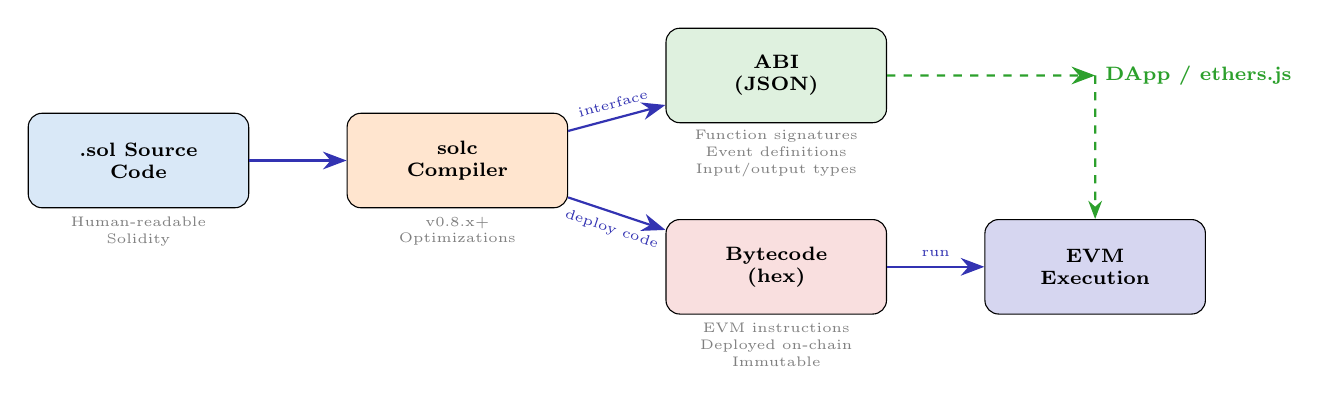
\begin{tikzpicture}[
  box/.style={draw,rounded corners=5pt,minimum width=2.8cm,minimum height=1.2cm,
    font=\scriptsize\bfseries,align=center},
  arr/.style={-{Stealth[length=3mm]},thick,mlpurple},
  scale=0.9
]
  % Source
  \node[box,fill=mlblue!15] (src) at (0,0) {.sol Source\\Code};
  \node[font=\tiny,mlgray,align=center] at (0,-1) {Human-readable\\Solidity};
  % Compiler
  \node[box,fill=mlorange!20] (comp) at (4.5,0) {solc\\Compiler};
  \node[font=\tiny,mlgray,align=center] at (4.5,-1) {v0.8.x+\\Optimizations};
  % ABI output
  \node[box,fill=mlgreen!15] (abi) at (9,1.2) {ABI\\(JSON)};
  \node[font=\tiny,mlgray,align=center] at (9,0.1) {Function signatures\\Event definitions\\Input/output types};
  % Bytecode output
  \node[box,fill=mlred!15] (byte) at (9,-1.5) {Bytecode\\(hex)};
  \node[font=\tiny,mlgray,align=center] at (9,-2.6) {EVM instructions\\Deployed on-chain\\Immutable};
  % EVM
  \node[box,fill=mlpurple!20] (evm) at (13.5,-1.5) {EVM\\Execution};
  % Arrows
  \draw[arr] (src) -- (comp);
  \draw[arr] (comp) -- (abi) node[midway,above,font=\tiny,sloped]{interface};
  \draw[arr] (comp) -- (byte) node[midway,below,font=\tiny,sloped]{deploy code};
  \draw[arr] (byte) -- (evm) node[midway,above,font=\tiny]{run};
  % DApp connection
  \draw[arr,mlgreen,dashed] (abi) -- (13.5,1.2) node[right,font=\scriptsize\bfseries,mlgreen]{DApp / ethers.js};
  \draw[-{Stealth},thick,mlgreen,dashed] (13.5,1.2) -- (evm);
\end{tikzpicture}
\end{center}
\vspace{2mm}
\begin{columns}
\column{0.32\textwidth}
\begin{block}{Language Features}
\begin{itemize}\small
  \item Statically typed
  \item Inheritance (multiple)
  \item Modifiers (decorators)
  \item Events for logging
  \item Error handling (require/revert)
\end{itemize}
\end{block}
\column{0.32\textwidth}
\begin{block}{Alternatives}
\begin{itemize}\small
  \item \textbf{Vyper}: Python-like, safer defaults
  \item \textbf{Yul}: Low-level, assembly-like
  \item \textbf{Huff}: Ultra-low-level, max gas efficiency
  \item \textbf{Fe}: Rust-inspired, experimental
\end{itemize}
\end{block}
\column{0.32\textwidth}
\begin{block}{Key Stats}
\begin{itemize}\small
  \item $\sim$90\% of contracts use Solidity
  \item $>$300K verified contracts on Etherscan
  \item Latest stable: v0.8.28
  \item Built-in overflow checks (0.8+)
\end{itemize}
\end{block}
\end{columns}
\bottomnote{The ABI (Application Binary Interface) is the contract's API -- it tells external callers how to encode function calls}
\end{frame}

%--- FRAME 24: Contract Structure ---
\begin{frame}[fragile]{Contract Structure}
\begin{columns}
\column{0.48\textwidth}
\begin{lstlisting}
// SPDX-License-Identifier: MIT
pragma solidity ^0.8.20;

import "@openzeppelin/contracts/access/Ownable.sol";

contract SimpleVault is Ownable {
  // State variables (storage)
  mapping(address => uint256) public balances;
  uint256 public totalDeposits;

  // Events
  event Deposit(address indexed user, uint256 amount);
  event Withdrawal(address indexed user, uint256 amount);

  // Constructor
  constructor() Ownable(msg.sender) {}
\end{lstlisting}
\column{0.48\textwidth}
\begin{lstlisting}
  // Modifier
  modifier hasBalance(uint256 amount) {
    require(balances[msg.sender] >= amount,
            "Insufficient balance");
    _;
  }

  // External function (payable)
  function deposit() external payable {
    balances[msg.sender] += msg.value;
    totalDeposits += msg.value;
    emit Deposit(msg.sender, msg.value);
  }

  // External function with modifier
  function withdraw(uint256 amount)
    external hasBalance(amount) {
    balances[msg.sender] -= amount;
    totalDeposits -= amount;
    payable(msg.sender).transfer(amount);
    emit Withdrawal(msg.sender, amount);
  }
}
\end{lstlisting}
\end{columns}
\vspace{2mm}
\begin{alertblock}{Anatomy Checklist}
\small \textbf{License} (SPDX) $\to$ \textbf{Pragma} (compiler version) $\to$ \textbf{Imports} $\to$ \textbf{Contract declaration} (inheritance) $\to$ \textbf{State variables} $\to$ \textbf{Events} $\to$ \textbf{Constructor} $\to$ \textbf{Modifiers} $\to$ \textbf{Functions}
\end{alertblock}
\bottomnote{Convention: state variables first, then events, constructor, modifiers, external/public, internal/private functions}
\end{frame}

%--- FRAME 25: Data Types Overview ---
\begin{frame}{Data Types Overview}
\begin{center}
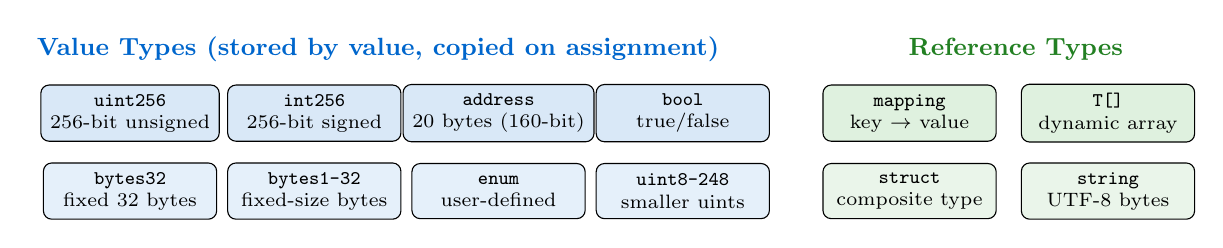
\begin{tikzpicture}[
  typebox/.style={draw,rounded corners=3pt,font=\scriptsize,align=center,
    minimum width=2.2cm,minimum height=0.7cm},
  scale=0.9
]
  % Value Types header
  \node[font=\small\bfseries,mlblue] at (3.5,3.5) {Value Types (stored by value, copied on assignment)};
  \node[typebox,fill=mlblue!15] at (0,2.6) {\texttt{uint256}\\256-bit unsigned};
  \node[typebox,fill=mlblue!15] at (2.6,2.6) {\texttt{int256}\\256-bit signed};
  \node[typebox,fill=mlblue!15] at (5.2,2.6) {\texttt{address}\\20 bytes (160-bit)};
  \node[typebox,fill=mlblue!15] at (7.8,2.6) {\texttt{bool}\\true/false};
  \node[typebox,fill=mlblue!10] at (0,1.5) {\texttt{bytes32}\\fixed 32 bytes};
  \node[typebox,fill=mlblue!10] at (2.6,1.5) {\texttt{bytes1-32}\\fixed-size bytes};
  \node[typebox,fill=mlblue!10] at (5.2,1.5) {\texttt{enum}\\user-defined};
  \node[typebox,fill=mlblue!10] at (7.8,1.5) {\texttt{uint8-248}\\smaller uints};
  % Reference Types header
  \node[font=\small\bfseries,mlgreen!80!black] at (12.5,3.5) {Reference Types};
  \node[typebox,fill=mlgreen!15] at (11,2.6) {\texttt{mapping}\\key $\to$ value};
  \node[typebox,fill=mlgreen!15] at (13.8,2.6) {\texttt{T[]}\\dynamic array};
  \node[typebox,fill=mlgreen!10] at (11,1.5) {\texttt{struct}\\composite type};
  \node[typebox,fill=mlgreen!10] at (13.8,1.5) {\texttt{string}\\UTF-8 bytes};
\end{tikzpicture}
\end{center}
\vspace{1mm}
\begin{columns}
\column{0.48\textwidth}
\begin{block}{Gas Cost by Type}
\small
\begin{tabular}{@{}llr@{}}
\toprule
\textbf{Type} & \textbf{Size} & \textbf{Storage Cost} \\
\midrule
\texttt{uint256} & 32 bytes (1 slot) & 20,000 gas \\
\texttt{address} & 20 bytes & 20,000 gas \\
\texttt{bool} & 1 byte (1 slot!) & 20,000 gas \\
\texttt{uint128 + uint128} & 32 bytes (1 slot) & 20,000 gas \\
\texttt{mapping} entry & 32 bytes/value & 20,000 gas \\
\bottomrule
\end{tabular}
\end{block}
\column{0.48\textwidth}
\begin{block}{Important Notes}
\begin{itemize}\small
  \item A \texttt{bool} alone wastes 31 bytes of a 32-byte slot
  \item Pack smaller types together: \texttt{uint128 + uint128} = 1 slot
  \item \texttt{mapping} keys are not iterable (no \texttt{.length})
  \item \texttt{string} is dynamically sized -- expensive for long strings
  \item \texttt{address payable} can receive ETH via \texttt{.transfer()}
\end{itemize}
\end{block}
\end{columns}
\bottomnote{EVM operates on 256-bit words -- smaller types save gas only when packed together in the same storage slot}
\end{frame}

%--- FRAME 26: Storage vs Memory vs Calldata ---
\begin{frame}{Storage vs Memory vs Calldata}
\begin{columns}
\column{0.55\textwidth}
\begin{center}
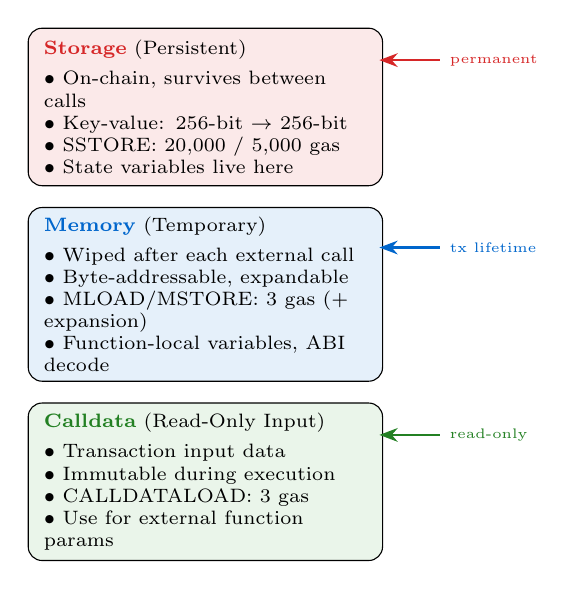
\begin{tikzpicture}[
  loc/.style={draw,rounded corners=5pt,minimum width=4.5cm,minimum height=2cm,
    font=\scriptsize,align=left,text width=4.1cm},
  scale=0.85
]
  % Storage
  \node[loc,fill=mlred!10] (st) at (0,3.5) {
    \textbf{\textcolor{mlred}{Storage}} (Persistent)\\[1mm]
    $\bullet$ On-chain, survives between calls\\
    $\bullet$ Key-value: 256-bit $\to$ 256-bit\\
    $\bullet$ SSTORE: 20,000 / 5,000 gas\\
    $\bullet$ State variables live here
  };
  % Memory
  \node[loc,fill=mlblue!10] (mem) at (0,0.7) {
    \textbf{\textcolor{mlblue}{Memory}} (Temporary)\\[1mm]
    $\bullet$ Wiped after each external call\\
    $\bullet$ Byte-addressable, expandable\\
    $\bullet$ MLOAD/MSTORE: 3 gas (+ expansion)\\
    $\bullet$ Function-local variables, ABI decode
  };
  % Calldata
  \node[loc,fill=mlgreen!10] (cd) at (0,-2.1) {
    \textbf{\textcolor{mlgreen!80!black}{Calldata}} (Read-Only Input)\\[1mm]
    $\bullet$ Transaction input data\\
    $\bullet$ Immutable during execution\\
    $\bullet$ CALLDATALOAD: 3 gas\\
    $\bullet$ Use for external function params
  };
  % Persistence arrows
  \draw[{Stealth}-,mlred,thick] (2.6,4.2) -- (3.5,4.2) node[right,font=\tiny]{permanent};
  \draw[{Stealth}-,mlblue,thick] (2.6,1.4) -- (3.5,1.4) node[right,font=\tiny]{tx lifetime};
  \draw[{Stealth}-,mlgreen!80!black,thick] (2.6,-1.4) -- (3.5,-1.4) node[right,font=\tiny]{read-only};
\end{tikzpicture}
\end{center}
\column{0.42\textwidth}
\begin{block}{Cost Comparison}
\small
\begin{tabular}{@{}lrr@{}}
\toprule
\textbf{Location} & \textbf{Read} & \textbf{Write} \\
\midrule
Storage (cold) & 2,100 & 20,000 \\
Storage (warm) & 100 & 5,000 \\
Memory & 3 & 3 \\
Calldata & 3 & -- \\
\bottomrule
\end{tabular}
\end{block}
\vspace{2mm}
\begin{block}{When to Use Each}
\begin{itemize}\small
  \item \textbf{Storage}: state that must persist (balances, ownership)
  \item \textbf{Memory}: intermediate computations, return values, struct construction
  \item \textbf{Calldata}: external function parameters that are read but not modified
\end{itemize}
\end{block}
\vspace{2mm}
\begin{alertblock}{Optimization Rule}
\small Cache storage reads in memory variables: read once from storage (2,100 gas), reuse from memory (3 gas).
\end{alertblock}
\end{columns}
\bottomnote{Stack (256-bit words, max depth 1024) is also a data location -- local value-type variables live on the stack for free}
\end{frame}

%--- FRAME 27: Functions & Visibility ---
\begin{frame}{Functions \& Visibility}
\begin{center}
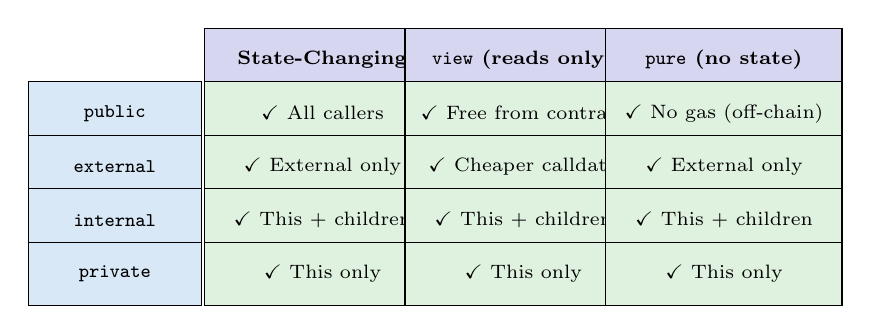
\begin{tikzpicture}[
  cell/.style={draw,minimum width=3cm,minimum height=0.8cm,font=\scriptsize,align=center},
  hdr/.style={cell,fill=mlpurple!20,font=\scriptsize\bfseries},
  rhdr/.style={cell,fill=mlblue!15,font=\scriptsize\bfseries,minimum width=2.2cm},
  yes/.style={cell,fill=mlgreen!15},
  no/.style={cell,fill=mlred!10},
  scale=0.85
]
  % Column headers
  \node[hdr] at (3.6,3) {State-Changing};
  \node[hdr] at (6.6,3) {\texttt{view} (reads only)};
  \node[hdr] at (9.6,3) {\texttt{pure} (no state)};
  % Row headers
  \node[rhdr] at (0.5,2.2) {\texttt{public}};
  \node[rhdr] at (0.5,1.4) {\texttt{external}};
  \node[rhdr] at (0.5,0.6) {\texttt{internal}};
  \node[rhdr] at (0.5,-0.2) {\texttt{private}};
  % Grid -- public row
  \node[yes] at (3.6,2.2) {$\checkmark$ All callers};
  \node[yes] at (6.6,2.2) {$\checkmark$ Free from contract};
  \node[yes] at (9.6,2.2) {$\checkmark$ No gas (off-chain)};
  % Grid -- external row
  \node[yes] at (3.6,1.4) {$\checkmark$ External only};
  \node[yes] at (6.6,1.4) {$\checkmark$ Cheaper calldata};
  \node[yes] at (9.6,1.4) {$\checkmark$ External only};
  % Grid -- internal row
  \node[yes] at (3.6,0.6) {$\checkmark$ This + children};
  \node[yes] at (6.6,0.6) {$\checkmark$ This + children};
  \node[yes] at (9.6,0.6) {$\checkmark$ This + children};
  % Grid -- private row
  \node[yes] at (3.6,-0.2) {$\checkmark$ This only};
  \node[yes] at (6.6,-0.2) {$\checkmark$ This only};
  \node[yes] at (9.6,-0.2) {$\checkmark$ This only};
\end{tikzpicture}
\end{center}
\vspace{1mm}
\begin{columns}
\column{0.48\textwidth}
\begin{block}{Visibility Rules}
\begin{itemize}\small
  \item \textbf{public}: callable by anyone; auto-generates getter for state vars
  \item \textbf{external}: only callable from outside (saves gas via \texttt{calldata})
  \item \textbf{internal}: this contract + derived contracts (like \texttt{protected})
  \item \textbf{private}: only this contract (not derived contracts)
\end{itemize}
\end{block}
\column{0.48\textwidth}
\begin{block}{State Mutability}
\begin{itemize}\small
  \item \textbf{(default)}: can read and write state, costs gas
  \item \textbf{view}: reads state but never modifies (free if called externally)
  \item \textbf{pure}: no state access at all (e.g., math utilities)
  \item \textbf{payable}: can receive ETH with the call
\end{itemize}
\end{block}
\end{columns}
\vspace{1mm}
\begin{alertblock}{Gas Tip}
\small \texttt{external} functions use \texttt{calldata} directly (no copy to memory), making them cheaper than \texttt{public} for array/struct parameters. Prefer \texttt{external} over \texttt{public} when the function is never called internally.
\end{alertblock}
\bottomnote{Visibility is enforced at the EVM level -- \texttt{private} data is still readable on-chain via storage slots!}
\end{frame}

%--- FRAME 28: Function Modifiers ---
\begin{frame}[fragile]{Function Modifiers}
\begin{columns}
\column{0.46\textwidth}
\begin{lstlisting}
// Access control modifier
modifier onlyOwner() {
  require(msg.sender == owner,
          "Not the owner");
  _;  // function body executes here
}

// Reentrancy guard modifier
modifier nonReentrant() {
  require(!locked, "Reentrant call");
  locked = true;
  _;  // function body
  locked = false;
}

// Usage: stacking modifiers
function withdraw(uint256 amount)
  external
  onlyOwner
  nonReentrant
{
  payable(msg.sender).transfer(amount);
}
\end{lstlisting}
\column{0.50\textwidth}
\begin{center}
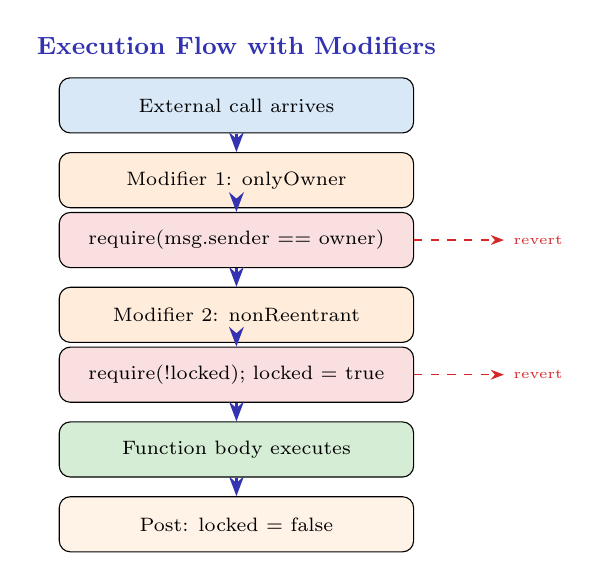
\begin{tikzpicture}[
  box/.style={draw,rounded corners=4pt,minimum width=4.5cm,minimum height=0.7cm,
    font=\scriptsize,align=center},
  arr/.style={-{Stealth[length=2.5mm]},thick,mlpurple},
  scale=0.95
]
  \node[font=\small\bfseries,mlpurple] at (0,3.8) {Execution Flow with Modifiers};
  \node[box,fill=mlblue!15] (call) at (0,3) {External call arrives};
  \node[box,fill=mlorange!15] (m1) at (0,2) {Modifier 1: onlyOwner};
  \node[box,fill=mlred!15] (chk1) at (0,1.2) {require(msg.sender == owner)};
  \node[box,fill=mlorange!15] (m2) at (0,0.2) {Modifier 2: nonReentrant};
  \node[box,fill=mlred!15] (chk2) at (0,-0.6) {require(!locked); locked = true};
  \node[box,fill=mlgreen!20] (body) at (0,-1.6) {Function body executes};
  \node[box,fill=mlorange!10] (post) at (0,-2.6) {Post: locked = false};
  % Arrows
  \draw[arr] (call) -- (m1);
  \draw[arr] (m1) -- (chk1);
  \draw[arr] (chk1) -- (m2);
  \draw[arr] (m2) -- (chk2);
  \draw[arr] (chk2) -- (body);
  \draw[arr] (body) -- (post);
  % Revert paths
  \draw[-{Stealth},mlred,dashed] (chk1.east) -- ++(1.2,0) node[right,font=\tiny,mlred]{revert};
  \draw[-{Stealth},mlred,dashed] (chk2.east) -- ++(1.2,0) node[right,font=\tiny,mlred]{revert};
\end{tikzpicture}
\end{center}
\end{columns}
\vspace{2mm}
\begin{alertblock}{Modifier Best Practices}
\small The \texttt{\_} placeholder marks where the function body is injected. Modifiers execute in declaration order (left to right). Keep modifiers short -- complex logic should be in separate internal functions for readability and reuse.
\end{alertblock}
\bottomnote{The Checks-Effects-Interactions pattern: (1) check conditions via require, (2) update state, (3) interact with externals}
\end{frame}

%--- FRAME 29: Events & Logging ---
\begin{frame}[fragile]{Events \& Logging}
\begin{columns}
\column{0.46\textwidth}
\begin{lstlisting}
// Event declaration (max 3 indexed)
event Transfer(
  address indexed from,
  address indexed to,
  uint256 value
);

event Approval(
  address indexed owner,
  address indexed spender,
  uint256 value
);

// Emitting events
function transfer(address to, uint256 amount)
  external returns (bool) {
  balances[msg.sender] -= amount;
  balances[to] += amount;
  emit Transfer(msg.sender, to, amount);
  return true;
}
\end{lstlisting}
\column{0.50\textwidth}
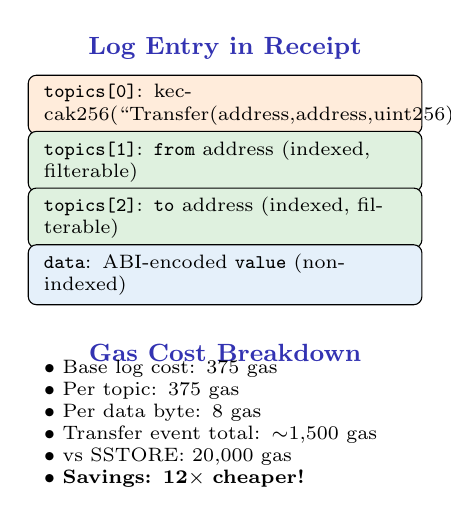
\begin{tikzpicture}[
  logbox/.style={draw,rounded corners=3pt,font=\scriptsize,align=left,
    minimum width=5cm,minimum height=0.5cm,text width=4.6cm},
  scale=0.9
]
  \node[font=\small\bfseries,mlpurple] at (0,3.5) {Log Entry in Receipt};
  \node[logbox,fill=mlorange!15] (t0) at (0,2.7) {
    \texttt{topics[0]}: keccak256(``Transfer(address,address,uint256)'')
  };
  \node[logbox,fill=mlgreen!15] (t1) at (0,1.9) {
    \texttt{topics[1]}: \texttt{from} address (indexed, filterable)
  };
  \node[logbox,fill=mlgreen!15] (t2) at (0,1.1) {
    \texttt{topics[2]}: \texttt{to} address (indexed, filterable)
  };
  \node[logbox,fill=mlblue!10] (data) at (0,0.3) {
    \texttt{data}: ABI-encoded \texttt{value} (non-indexed)
  };
  % Cost breakdown
  \node[font=\small\bfseries,mlpurple] at (0,-0.8) {Gas Cost Breakdown};
  \node[font=\scriptsize,align=left,text width=4.6cm] at (0,-1.8) {
    $\bullet$ Base log cost: 375 gas\\
    $\bullet$ Per topic: 375 gas\\
    $\bullet$ Per data byte: 8 gas\\
    $\bullet$ Transfer event total: $\sim$1,500 gas\\
    $\bullet$ vs SSTORE: 20,000 gas\\
    $\bullet$ \textbf{Savings: 12$\times$ cheaper!}
  };
\end{tikzpicture}
\end{columns}
\vspace{2mm}
\begin{alertblock}{When to Use Events vs Storage}
\small Use \textbf{events} for data that only needs off-chain access (audit trails, UI updates, historical queries). Use \textbf{storage} only for data that contracts need to read on-chain. Events are not accessible from within smart contracts.
\end{alertblock}
\bottomnote{DApps use ethers.js \texttt{contract.on(``Transfer'', callback)} to listen for events in real-time via WebSocket}
\end{frame}

%--- FRAME 30: Mappings & Arrays ---
\begin{frame}{Mappings \& Arrays: Storage Layout}
\begin{columns}
\column{0.52\textwidth}
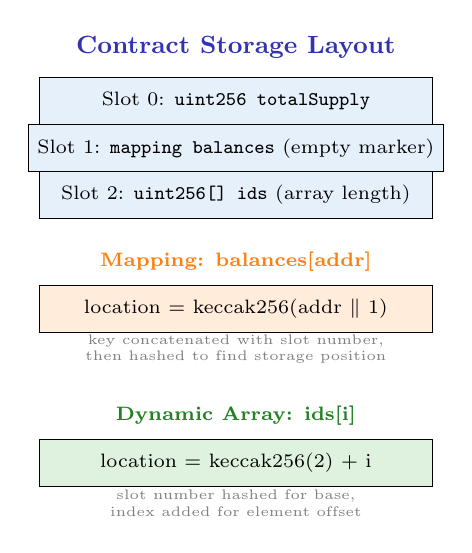
\begin{tikzpicture}[
  slot/.style={draw,minimum width=5cm,minimum height=0.6cm,font=\scriptsize,align=center},
  arr/.style={-{Stealth[length=2.5mm]},thick,mlpurple},
  scale=0.85
]
  % Storage slots
  \node[font=\small\bfseries,mlpurple] at (0,4.5) {Contract Storage Layout};
  \node[slot,fill=mlblue!10] (s0) at (0,3.7) {Slot 0: \texttt{uint256 totalSupply}};
  \node[slot,fill=mlblue!10] (s1) at (0,3.0) {Slot 1: \texttt{mapping balances} (empty marker)};
  \node[slot,fill=mlblue!10] (s2) at (0,2.3) {Slot 2: \texttt{uint256[] ids} (array length)};
  % Mapping access
  \node[font=\scriptsize\bfseries,mlorange] at (0,1.3) {Mapping: balances[addr]};
  \node[slot,fill=mlorange!15] (m1) at (0,0.6) {location = keccak256(addr $\|$ 1)};
  \node[font=\tiny,mlgray,align=center] at (0,0.0) {key concatenated with slot number,\\then hashed to find storage position};
  % Array access
  \node[font=\scriptsize\bfseries,mlgreen!80!black] at (0,-1.0) {Dynamic Array: ids[i]};
  \node[slot,fill=mlgreen!15] (a1) at (0,-1.7) {location = keccak256(2) + i};
  \node[font=\tiny,mlgray,align=center] at (0,-2.3) {slot number hashed for base,\\index added for element offset};
\end{tikzpicture}
\column{0.44\textwidth}
\begin{block}{Mapping Properties}
\begin{itemize}\small
  \item No iteration (no \texttt{.length}, no \texttt{.keys()})
  \item All keys implicitly exist (default: 0/false)
  \item Cannot be returned from functions
  \item Nested: \texttt{mapping(a => mapping(b => v))}
  \item Storage position: deterministic via keccak256
\end{itemize}
\end{block}
\vspace{2mm}
\begin{block}{Dynamic Array Properties}
\begin{itemize}\small
  \item \texttt{.push()}, \texttt{.pop()}, \texttt{.length}
  \item Elements stored contiguously from keccak256(slot)
  \item Iteration possible but gas scales linearly
  \item Deletion leaves gaps (use swap-and-pop pattern)
\end{itemize}
\end{block}
\vspace{2mm}
\begin{alertblock}{Design Pattern}
\small Combine mapping + array for iterable mappings: \texttt{mapping(addr => uint)} for O(1) lookup + \texttt{address[]} for enumeration.
\end{alertblock}
\end{columns}
\bottomnote{Storage slot collision is impossible in practice: keccak256 has 256-bit output space ($2^{256}$ possible positions)}
\end{frame}

%--- FRAME 31: Inheritance & Interfaces ---
\begin{frame}{Inheritance \& Interfaces}
\begin{columns}
\column{0.52\textwidth}
\begin{center}
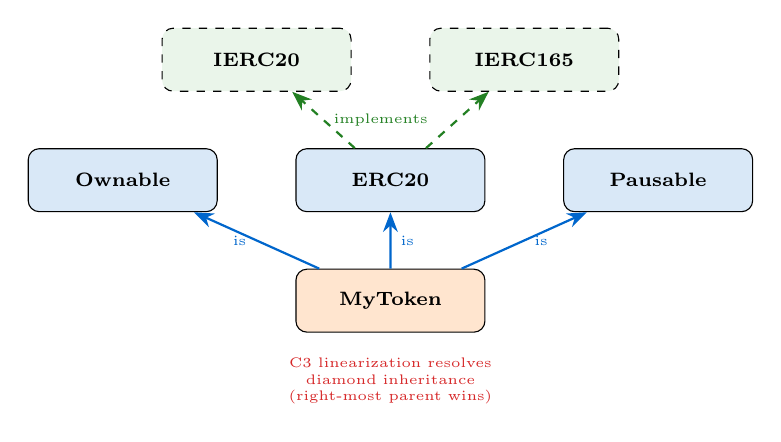
\begin{tikzpicture}[
  cls/.style={draw,rounded corners=4pt,minimum width=2.4cm,minimum height=0.8cm,
    font=\scriptsize\bfseries,align=center},
  iface/.style={draw,rounded corners=4pt,dashed,minimum width=2.4cm,minimum height=0.8cm,
    font=\scriptsize\bfseries,align=center},
  arr/.style={-{Stealth[length=2.5mm]},thick},
  scale=0.85
]
  % Interfaces
  \node[iface,fill=mlgreen!10] (ierc20) at (0,4) {IERC20};
  \node[iface,fill=mlgreen!10] (ierc165) at (4,4) {IERC165};
  % Base contracts
  \node[cls,fill=mlblue!15] (own) at (-2,2.2) {Ownable};
  \node[cls,fill=mlblue!15] (erc20) at (2,2.2) {ERC20};
  \node[cls,fill=mlblue!15] (pause) at (6,2.2) {Pausable};
  % Derived
  \node[cls,fill=mlorange!20] (token) at (2,0.4) {MyToken};
  % Arrows (inheritance)
  \draw[arr,mlblue] (token) -- (own) node[midway,left,font=\tiny]{is};
  \draw[arr,mlblue] (token) -- (erc20) node[midway,right,font=\tiny]{is};
  \draw[arr,mlblue] (token) -- (pause) node[midway,right,font=\tiny]{is};
  \draw[arr,mlgreen!80!black,dashed] (erc20) -- (ierc20) node[midway,right,font=\tiny]{implements};
  \draw[arr,mlgreen!80!black,dashed] (erc20) -- (ierc165);
  % Diamond label
  \node[font=\tiny,mlred,align=center,text width=3cm] at (2,-0.8) {C3 linearization resolves\\diamond inheritance\\(right-most parent wins)};
\end{tikzpicture}
\end{center}
\vspace{1mm}
\begin{block}{C3 Linearization}
\small For \texttt{contract MyToken is Ownable, ERC20, Pausable}: resolution order is MyToken $\to$ Pausable $\to$ ERC20 $\to$ Ownable. The \textbf{rightmost} parent is checked first when resolving \texttt{super} calls.
\end{block}
\column{0.44\textwidth}
\begin{block}{Interfaces}
\begin{itemize}\small
  \item Define function signatures without implementation
  \item Cannot have state variables or constructors
  \item All functions must be \texttt{external}
  \item Enable polymorphism and loose coupling
  \item ERC standards defined as interfaces (IERC20, IERC721)
\end{itemize}
\end{block}
\vspace{2mm}
\begin{block}{Abstract Contracts}
\begin{itemize}\small
  \item Can have both implemented and unimplemented functions
  \item Cannot be deployed directly
  \item Use \texttt{virtual} for overridable functions
  \item Use \texttt{override} in derived contracts
\end{itemize}
\end{block}
\vspace{2mm}
\begin{block}{Key ERC Interfaces}
\small
\begin{tabular}{@{}ll@{}}
\toprule
\textbf{Standard} & \textbf{Purpose} \\
\midrule
ERC-20 & Fungible tokens \\
ERC-721 & Non-fungible tokens \\
ERC-1155 & Multi-token standard \\
ERC-4626 & Tokenized vaults \\
\bottomrule
\end{tabular}
\end{block}
\end{columns}
\bottomnote{OpenZeppelin provides battle-tested implementations of all major ERC standards -- always prefer audited code}
\end{frame}

%--- FRAME 32: Error Handling ---
\begin{frame}{Error Handling}
\begin{center}
\small
\begin{tabular}{@{}p{2.5cm}p{3.8cm}p{3.8cm}p{3.8cm}@{}}
\toprule
& \textbf{\texttt{require(cond, msg)}} & \textbf{\texttt{assert(cond)}} & \textbf{\texttt{revert CustomError()}} \\
\midrule
\textbf{Purpose} & Input validation, access control, preconditions & Invariant checks, internal bugs & Custom errors with parameters (0.8.4+) \\
\textbf{Gas on failure} & Refunds remaining gas & Consumes \textbf{all} remaining gas (pre-0.8.0); refunds (0.8.0+) & Refunds remaining gas \\
\textbf{Use when} & External input might be invalid & Condition should \emph{never} be false & Need typed errors with data \\
\textbf{Error data} & String message (expensive) & Panic(uint256) error code & 4-byte selector + ABI params \\
\textbf{Gas cost} & $\sim$2,500 + string storage & $\sim$2,500 (0.8+) & $\sim$150 (just selector!) \\
\textbf{Example} & \texttt{require(bal >= amt, "Low")} & \texttt{assert(supply == sum)} & \texttt{revert InsufficientBalance()} \\
\bottomrule
\end{tabular}
\end{center}
\vspace{2mm}
\begin{columns}
\column{0.48\textwidth}
\begin{block}{Custom Errors (Recommended)}
\begin{itemize}\small
  \item Defined at contract level: \texttt{error InsufficientBalance(uint256 available, uint256 required)}
  \item Save $\sim$90\% gas vs string revert messages
  \item ABI-encodable, can carry context data
  \item Supported by all modern tooling (ethers.js, Foundry)
\end{itemize}
\end{block}
\column{0.48\textwidth}
\begin{block}{try/catch (External Calls)}
\begin{itemize}\small
  \item Catches reverts from \textbf{external} calls only
  \item Cannot catch errors in the same contract
  \item Catch clauses: \texttt{Error(string)}, \texttt{Panic(uint256)}, generic \texttt{(bytes)}
  \item Essential for composability with untrusted contracts
\end{itemize}
\end{block}
\end{columns}
\vspace{1mm}
\begin{alertblock}{Migration Path}
\small Replace \texttt{require(cond, "string")} with custom errors for 90\% gas savings on reverts. Solidity 0.8.26+ supports \texttt{require(cond, CustomError())}.
\end{alertblock}
\bottomnote{Error selectors are the first 4 bytes of keccak256 of the error signature -- same pattern as function selectors}
\end{frame}

%--- FRAME 33: Common Design Patterns ---
\begin{frame}{Common Design Patterns}
\begin{center}
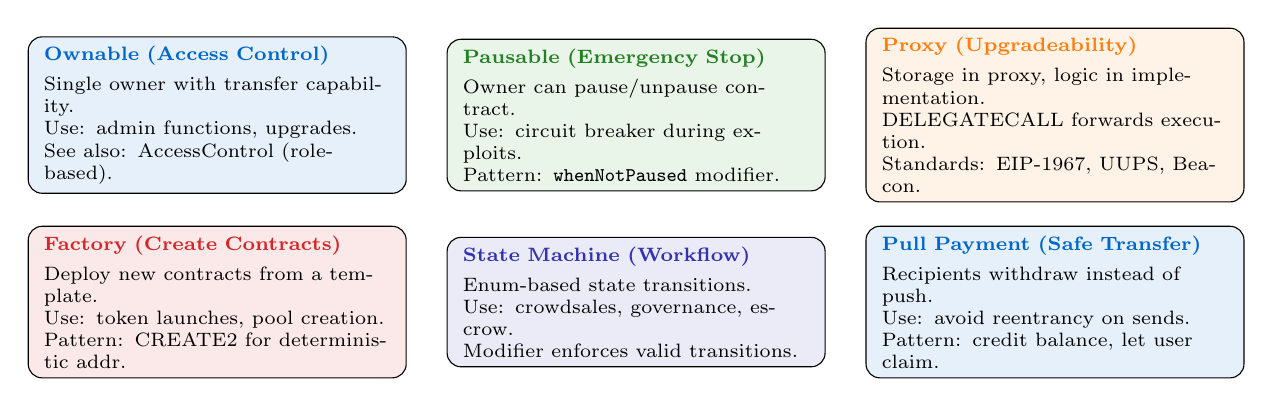
\begin{tikzpicture}[
  card/.style={draw,rounded corners=5pt,minimum width=4.8cm,minimum height=1.6cm,
    font=\scriptsize,align=left,text width=4.4cm},
  scale=0.95
]
  % Row 1
  \node[card,fill=mlblue!10] at (0,2) {
    \textbf{\textcolor{mlblue}{Ownable (Access Control)}}\\[1mm]
    Single owner with transfer capability.\\
    Use: admin functions, upgrades.\\
    See also: AccessControl (role-based).
  };
  \node[card,fill=mlgreen!10] at (5.6,2) {
    \textbf{\textcolor{mlgreen!80!black}{Pausable (Emergency Stop)}}\\[1mm]
    Owner can pause/unpause contract.\\
    Use: circuit breaker during exploits.\\
    Pattern: \texttt{whenNotPaused} modifier.
  };
  \node[card,fill=mlorange!10] at (11.2,2) {
    \textbf{\textcolor{mlorange}{Proxy (Upgradeability)}}\\[1mm]
    Storage in proxy, logic in implementation.\\
    DELEGATECALL forwards execution.\\
    Standards: EIP-1967, UUPS, Beacon.
  };
  % Row 2
  \node[card,fill=mlred!10] at (0,-0.5) {
    \textbf{\textcolor{mlred}{Factory (Create Contracts)}}\\[1mm]
    Deploy new contracts from a template.\\
    Use: token launches, pool creation.\\
    Pattern: CREATE2 for deterministic addr.
  };
  \node[card,fill=mlpurple!10] at (5.6,-0.5) {
    \textbf{\textcolor{mlpurple}{State Machine (Workflow)}}\\[1mm]
    Enum-based state transitions.\\
    Use: crowdsales, governance, escrow.\\
    Modifier enforces valid transitions.
  };
  \node[card,fill=mlblue!10] at (11.2,-0.5) {
    \textbf{\textcolor{mlblue}{Pull Payment (Safe Transfer)}}\\[1mm]
    Recipients withdraw instead of push.\\
    Use: avoid reentrancy on sends.\\
    Pattern: credit balance, let user claim.
  };
\end{tikzpicture}
\end{center}
\vspace{2mm}
\begin{columns}
\column{0.48\textwidth}
\begin{block}{OpenZeppelin Contracts}
\begin{itemize}\small
  \item Industry-standard library of audited patterns
  \item Ownable, AccessControl, Pausable, ReentrancyGuard
  \item ERC20, ERC721, ERC1155 implementations
  \item Governor (on-chain governance), TimelockController
\end{itemize}
\end{block}
\column{0.48\textwidth}
\begin{alertblock}{Pattern Selection Guide}
\small
\begin{tabular}{@{}ll@{}}
Need admin control? & Ownable / AccessControl \\
Need upgrades? & UUPS Proxy \\
Need emergency stop? & Pausable \\
Deploying many copies? & Factory + EIP-1167 \\
Complex workflow? & State Machine \\
\end{tabular}
\end{alertblock}
\end{columns}
\bottomnote{``Don't roll your own crypto, don't roll your own access control'' -- always use audited libraries like OpenZeppelin}
\end{frame}

%--- FRAME 34: Solidity Section Summary ---
\begin{frame}{Solidity Basics: Quick Reference}
\begin{columns}
\column{0.48\textwidth}
\begin{block}{Type System}
\colorbox{mlblue!10}{\parbox{0.92\linewidth}{\small
\textbf{Value types}: \texttt{uint256}, \texttt{int256}, \texttt{address}, \texttt{bool}, \texttt{bytes32}\\
\textbf{Reference types}: \texttt{mapping}, \texttt{array[]}, \texttt{struct}, \texttt{string}\\
\textbf{Locations}: \texttt{storage} (persistent) | \texttt{memory} (temp) | \texttt{calldata} (read-only)
}}
\end{block}
\vspace{1mm}
\begin{block}{Functions}
\colorbox{mlgreen!10}{\parbox{0.92\linewidth}{\small
\textbf{Visibility}: \texttt{public} | \texttt{external} | \texttt{internal} | \texttt{private}\\
\textbf{Mutability}: (default) | \texttt{view} | \texttt{pure} | \texttt{payable}\\
\textbf{Modifiers}: \texttt{onlyOwner}, \texttt{nonReentrant}, custom\\
\textbf{Tip}: prefer \texttt{external} + \texttt{calldata} for gas savings
}}
\end{block}
\vspace{1mm}
\begin{block}{Error Handling}
\colorbox{mlred!10}{\parbox{0.92\linewidth}{\small
\texttt{require(cond, msg)} -- input validation\\
\texttt{revert CustomError()} -- gas-efficient (0.8.4+)\\
\texttt{assert(cond)} -- invariant checks\\
\texttt{try/catch} -- external call safety
}}
\end{block}
\column{0.48\textwidth}
\begin{block}{Events}
\colorbox{mlorange!10}{\parbox{0.92\linewidth}{\small
\texttt{event Transfer(address indexed from, address indexed to, uint256 value)}\\
Max 3 indexed params (topics), rest in data\\
12$\times$ cheaper than storage for historical records
}}
\end{block}
\vspace{1mm}
\begin{block}{Storage Layout}
\colorbox{mlpurple!10}{\parbox{0.92\linewidth}{\small
Each slot = 256 bits = 32 bytes\\
Mapping: \texttt{keccak256(key || slot)}\\
Dynamic array: \texttt{keccak256(slot) + index}\\
Pack small types: \texttt{uint128 + uint128} = 1 slot
}}
\end{block}
\vspace{1mm}
\begin{block}{Design Patterns}
\colorbox{mlblue!10}{\parbox{0.92\linewidth}{\small
Ownable (access) | Pausable (emergency)\\
Proxy (upgrades) | Factory (deploy)\\
State Machine (workflow) | Pull Payment (safety)\\
\textbf{Always use OpenZeppelin for standard patterns}
}}
\end{block}
\vspace{1mm}
\begin{alertblock}{Next Section}
\small Deploy \& Interact: Remix IDE, Hardhat framework, testing with Foundry, mainnet deployment workflow.
\end{alertblock}
\end{columns}
\bottomnote{Solidity mastery = types + storage optimization + security patterns -- the rest is syntax}
\end{frame}

%--- Sections 4-5 will be appended below this line ---

\section{Deploy and Interact}

%--- FRAME 35: Development Environment ---
\begin{frame}{Development Environment}
\begin{center}
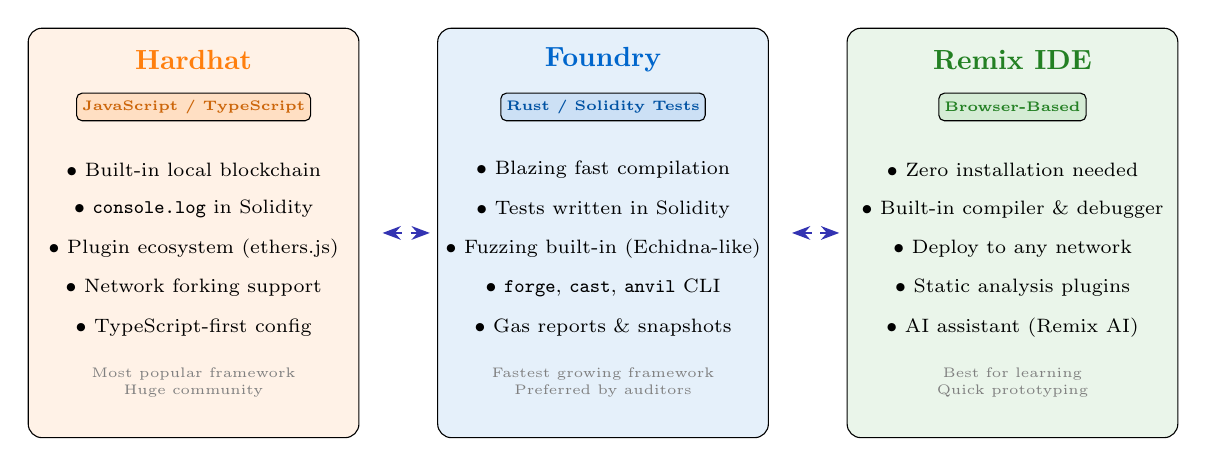
\begin{tikzpicture}[
  toolcard/.style={draw,rounded corners=5pt,minimum width=4.2cm,minimum height=5.2cm,
    font=\small,align=center},
  feat/.style={font=\scriptsize,align=left},
  badge/.style={draw,rounded corners=2pt,font=\tiny\bfseries,inner sep=2pt,minimum height=0.35cm}
]
  % Hardhat
  \node[toolcard,fill=mlorange!10] (hh) at (0,0) {};
  \node[font=\normalsize\bfseries,mlorange] at (0,2.2) {Hardhat};
  \node[badge,fill=mlorange!25,text=mlorange!80!black] at (0,1.6) {JavaScript / TypeScript};
  \node[feat] at (0,0.8) {$\bullet$ Built-in local blockchain};
  \node[feat] at (0,0.3) {$\bullet$ \texttt{console.log} in Solidity};
  \node[feat] at (0,-0.2) {$\bullet$ Plugin ecosystem (ethers.js)};
  \node[feat] at (0,-0.7) {$\bullet$ Network forking support};
  \node[feat] at (0,-1.2) {$\bullet$ TypeScript-first config};
  \node[font=\tiny,mlgray,align=center] at (0,-1.9) {Most popular framework\\Huge community};

  % Foundry
  \node[toolcard,fill=mlblue!10] (fo) at (5.2,0) {};
  \node[font=\normalsize\bfseries,mlblue] at (5.2,2.2) {Foundry};
  \node[badge,fill=mlblue!20,text=mlblue!80!black] at (5.2,1.6) {Rust / Solidity Tests};
  \node[feat] at (5.2,0.8) {$\bullet$ Blazing fast compilation};
  \node[feat] at (5.2,0.3) {$\bullet$ Tests written in Solidity};
  \node[feat] at (5.2,-0.2) {$\bullet$ Fuzzing built-in (Echidna-like)};
  \node[feat] at (5.2,-0.7) {$\bullet$ \texttt{forge}, \texttt{cast}, \texttt{anvil} CLI};
  \node[feat] at (5.2,-1.2) {$\bullet$ Gas reports \& snapshots};
  \node[font=\tiny,mlgray,align=center] at (5.2,-1.9) {Fastest growing framework\\Preferred by auditors};

  % Remix
  \node[toolcard,fill=mlgreen!10] (rm) at (10.4,0) {};
  \node[font=\normalsize\bfseries,mlgreen!80!black] at (10.4,2.2) {Remix IDE};
  \node[badge,fill=mlgreen!20,text=mlgreen!80!black] at (10.4,1.6) {Browser-Based};
  \node[feat] at (10.4,0.8) {$\bullet$ Zero installation needed};
  \node[feat] at (10.4,0.3) {$\bullet$ Built-in compiler \& debugger};
  \node[feat] at (10.4,-0.2) {$\bullet$ Deploy to any network};
  \node[feat] at (10.4,-0.7) {$\bullet$ Static analysis plugins};
  \node[feat] at (10.4,-1.2) {$\bullet$ AI assistant (Remix AI)};
  \node[font=\tiny,mlgray,align=center] at (10.4,-1.9) {Best for learning\\Quick prototyping};

  % Connecting arrows
  \draw[{Stealth}-{Stealth},thick,mlpurple,dashed] (2.4,0) -- (3,0);
  \draw[{Stealth}-{Stealth},thick,mlpurple,dashed] (7.6,0) -- (8.2,0);
\end{tikzpicture}
\end{center}
\bottomnote{Start with Remix for learning, graduate to Hardhat/Foundry for production -- many teams use Foundry for tests + Hardhat for scripts}
\end{frame}

%--- FRAME 36: Compilation Process ---
\begin{frame}{Compilation Process}
\begin{center}
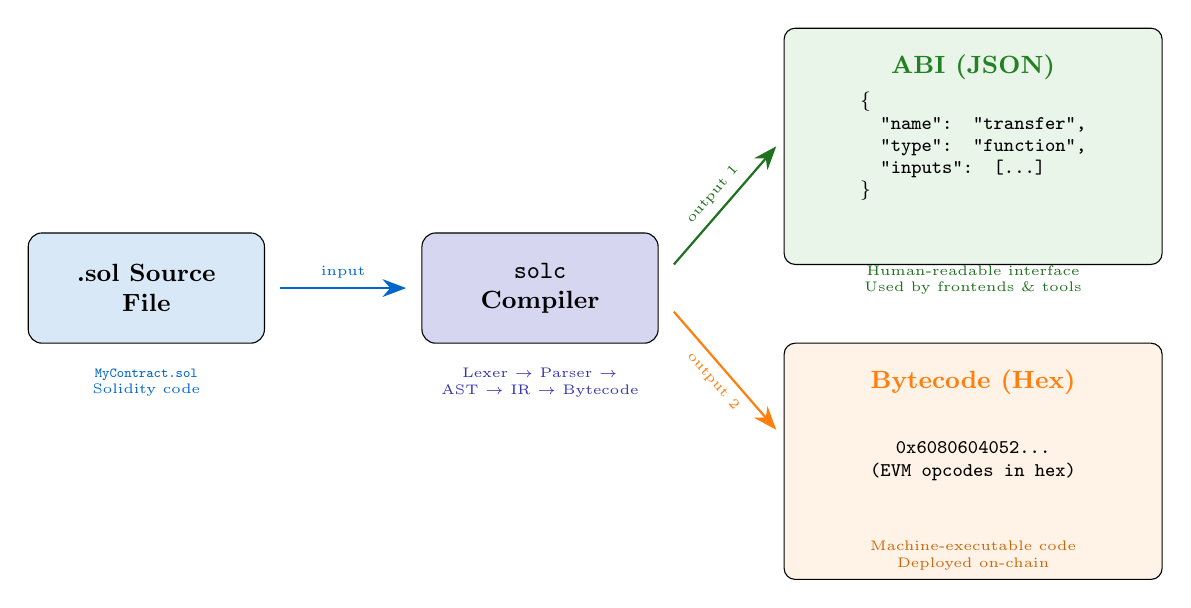
\begin{tikzpicture}[
  procbox/.style={draw,rounded corners=5pt,minimum width=3cm,minimum height=1.4cm,
    font=\small\bfseries,align=center},
  outbox/.style={draw,rounded corners=4pt,minimum width=4.8cm,minimum height=3cm,
    font=\small,align=center},
  arr/.style={-{Stealth[length=3mm]},thick},
  note/.style={font=\tiny,align=center}
]
  % Source file
  \node[procbox,fill=mlblue!15] (src) at (0,0) {.sol Source\\File};
  \node[note,mlblue] at (0,-1.2) {\texttt{MyContract.sol}\\Solidity code};

  % Compiler
  \node[procbox,fill=mlpurple!20] (solc) at (5,0) {\texttt{solc}\\Compiler};
  \node[note,mlpurple] at (5,-1.2) {Lexer $\to$ Parser $\to$\\AST $\to$ IR $\to$ Bytecode};

  % ABI output
  \node[outbox,fill=mlgreen!10] (abi) at (10.5,1.8) {};
  \node[font=\small\bfseries,mlgreen!80!black] at (10.5,2.8) {ABI (JSON)};
  \node[font=\scriptsize,align=left] at (10.5,1.8) {
    \texttt{\{} \\
    \texttt{~~"name": "transfer",}\\
    \texttt{~~"type": "function",}\\
    \texttt{~~"inputs": [...]}\\
    \texttt{\}}
  };
  \node[note,mlgreen!70!black] at (10.5,0.1) {Human-readable interface\\Used by frontends \& tools};

  % Bytecode output
  \node[outbox,fill=mlorange!10] (byte) at (10.5,-2.2) {};
  \node[font=\small\bfseries,mlorange] at (10.5,-1.2) {Bytecode (Hex)};
  \node[font=\scriptsize,align=center] at (10.5,-2.2) {
    \texttt{0x6080604052...}\\
    \texttt{(EVM opcodes in hex)}
  };
  \node[note,mlorange!80!black] at (10.5,-3.4) {Machine-executable code\\Deployed on-chain};

  % Arrows
  \draw[arr,mlblue] (1.7,0) -- (3.3,0) node[midway,above,font=\tiny]{input};
  \draw[arr,mlgreen!70!black] (6.7,0.3) -- (8,1.8) node[midway,above,font=\tiny,sloped]{output 1};
  \draw[arr,mlorange] (6.7,-0.3) -- (8,-1.8) node[midway,below,font=\tiny,sloped]{output 2};
\end{tikzpicture}
\end{center}
\vspace{2mm}
\begin{columns}
\column{0.48\textwidth}
\begin{block}{Compiler Versions Matter}
\begin{itemize}\small
  \item \texttt{pragma solidity \^{}0.8.20;} locks version range
  \item Each version fixes bugs and adds features
  \item 0.8.0: built-in overflow checks
  \item 0.8.24: transient storage (\texttt{TSTORE}/\texttt{TLOAD})
\end{itemize}
\end{block}
\column{0.48\textwidth}
\begin{alertblock}{Two Outputs, Two Purposes}
\small \textbf{ABI}: tells the \emph{outside world} how to talk to the contract (function signatures, parameter types).\\[2mm]
\textbf{Bytecode}: tells the \emph{EVM} what to execute (low-level stack operations encoded in hex).
\end{alertblock}
\end{columns}
\bottomnote{Compiler optimizations (\texttt{--optimize --runs 200}) reduce deployment gas but increase compilation time}
\end{frame}

%--- FRAME 37: ABI: The Contract Interface ---
\begin{frame}{ABI: The Contract Interface}
\begin{center}
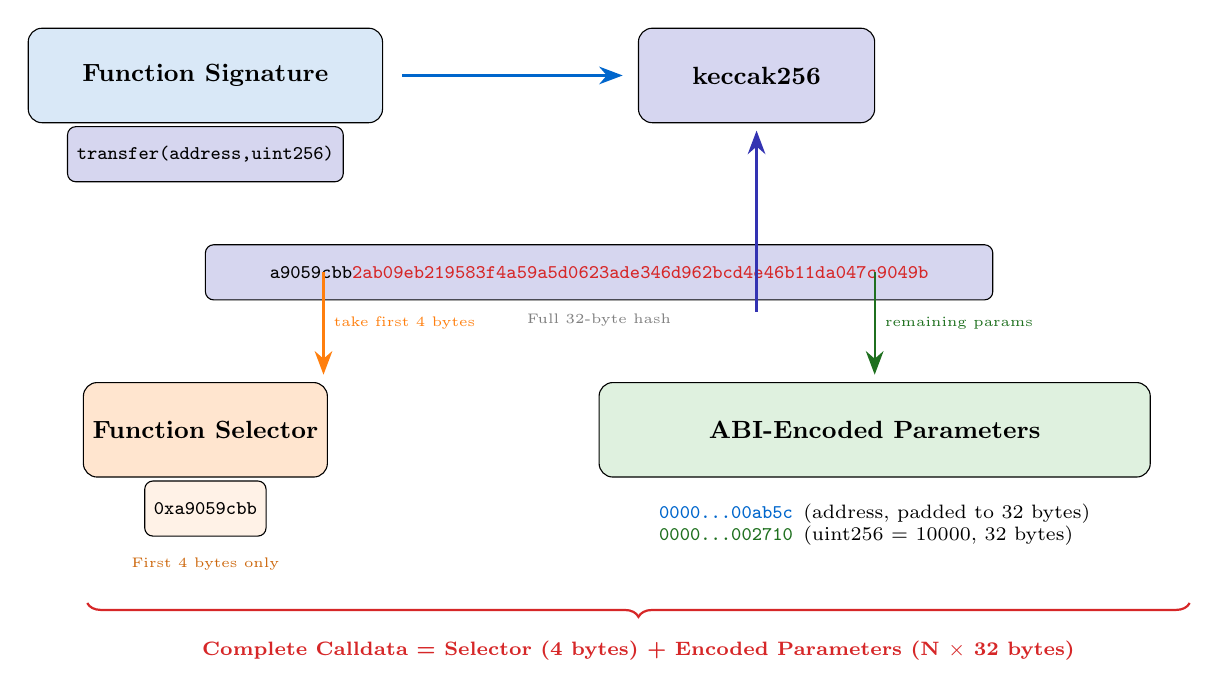
\begin{tikzpicture}[
  procbox/.style={draw,rounded corners=5pt,minimum height=1.2cm,font=\small\bfseries,align=center},
  databox/.style={draw,rounded corners=3pt,fill=mllavender4,font=\scriptsize\ttfamily,
    minimum height=0.7cm,align=center},
  arr/.style={-{Stealth[length=3mm]},thick},
  note/.style={font=\tiny,align=center}
]
  % Function signature
  \node[procbox,fill=mlblue!15,minimum width=4.5cm] (sig) at (0,2.5) {Function Signature};
  \node[databox] at (0,1.5) {transfer(address,uint256)};

  % Keccak
  \node[procbox,fill=mlpurple!20,minimum width=3cm] (hash) at (7,2.5) {keccak256};

  % Full hash
  \node[databox,minimum width=10cm] (full) at (5,0) {a9059cbb\textcolor{mlred}{2ab09eb219583f4a59a5d0623ade346d962bcd4e46b11da047c9049b}};
  \node[note,mlgray] at (5,-0.6) {Full 32-byte hash};

  % Selector
  \node[procbox,fill=mlorange!20,minimum width=3cm] (sel) at (0,-2) {Function Selector};
  \node[databox,fill=mlorange!10] at (0,-3) {0xa9059cbb};
  \node[note,mlorange!80!black] at (0,-3.7) {First 4 bytes only};

  % Parameters
  \node[procbox,fill=mlgreen!15,minimum width=7cm] (params) at (8.5,-2) {ABI-Encoded Parameters};
  \node[font=\scriptsize\ttfamily,align=left] at (8.5,-3.2) {
    \textcolor{mlblue}{0000...00ab5c} {\scriptsize\rmfamily (address, padded to 32 bytes)}\\
    \textcolor{mlgreen!70!black}{0000...002710} {\scriptsize\rmfamily (uint256 = 10000, 32 bytes)}
  };

  % Arrows
  \draw[arr,mlblue] (2.5,2.5) -- (5.3,2.5);
  \draw[arr,mlpurple] (7,-0.5) -- (7,1.8);
  \draw[arr,mlorange] (1.5,0) -- (1.5,-1.3) node[midway,right,font=\tiny]{take first 4 bytes};
  \draw[arr,mlgreen!70!black] (8.5,0) -- (8.5,-1.3) node[midway,right,font=\tiny]{remaining params};

  % Calldata assembly
  \draw[decorate,decoration={brace,amplitude=5pt,mirror},thick,mlred] (-1.5,-4.2) -- (12.5,-4.2);
  \node[font=\scriptsize\bfseries,mlred] at (5.5,-4.8) {Complete Calldata = Selector (4 bytes) + Encoded Parameters (N $\times$ 32 bytes)};
\end{tikzpicture}
\end{center}
\bottomnote{ABI encoding uses 32-byte words for all types -- even a \texttt{bool} occupies 32 bytes in calldata}
\end{frame}

%--- FRAME 38: Deployment Transaction ---
\begin{frame}{Deployment Transaction}
\begin{center}
\adjustbox{max width=\textwidth}{%
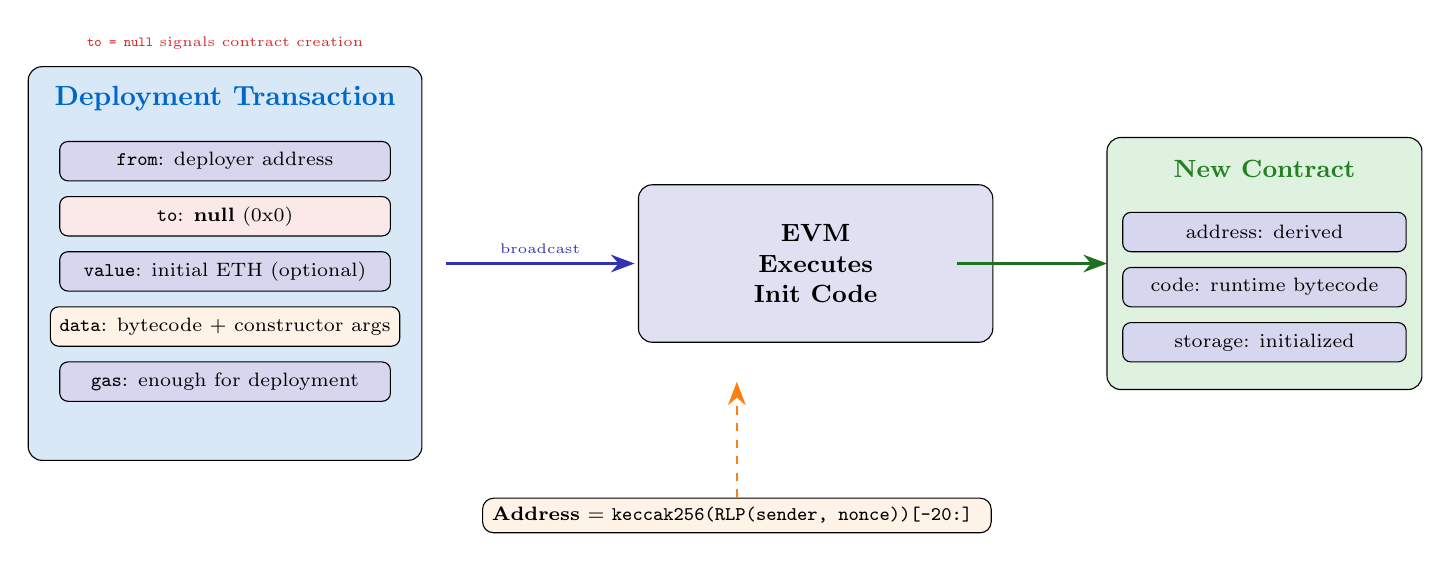
\begin{tikzpicture}[
  txbox/.style={draw,rounded corners=5pt,minimum width=4.5cm,minimum height=1cm,
    font=\small\bfseries,align=center},
  field/.style={draw,rounded corners=3pt,fill=mllavender4,font=\scriptsize,
    minimum width=4.2cm,minimum height=0.5cm,align=left},
  arr/.style={-{Stealth[length=3mm]},thick},
  note/.style={font=\tiny,align=center}
]
  % Deployment TX
  \node[txbox,fill=mlblue!15,minimum height=5cm,minimum width=5cm] (tx) at (0,0) {};
  \node[font=\normalsize\bfseries,mlblue] at (0,2.1) {Deployment Transaction};
  \node[field] at (0,1.3) {\texttt{from}: deployer address};
  \node[field,fill=mlred!10] at (0,0.6) {\texttt{to}: \textbf{null} (0x0)};
  \node[field] at (0,-0.1) {\texttt{value}: initial ETH (optional)};
  \node[field,fill=mlorange!10] at (0,-0.8) {\texttt{data}: bytecode + constructor args};
  \node[field] at (0,-1.5) {\texttt{gas}: enough for deployment};

  % Arrow to network
  \draw[arr,mlpurple] (2.8,0) -- (5.2,0) node[midway,above,font=\tiny]{broadcast};

  % EVM processing
  \node[txbox,fill=mlpurple!15,minimum height=2cm] (evm) at (7.5,0) {EVM\\Executes\\Init Code};

  % Arrow to contract born
  \draw[arr,mlgreen!70!black] (9.3,0) -- (11.2,0);

  % New contract
  \node[txbox,fill=mlgreen!15,minimum height=3.2cm,minimum width=4cm] (contract) at (13.2,0) {};
  \node[font=\small\bfseries,mlgreen!80!black] at (13.2,1.2) {New Contract};
  \node[field,minimum width=3.6cm] at (13.2,0.4) {address: derived};
  \node[field,minimum width=3.6cm] at (13.2,-0.3) {code: runtime bytecode};
  \node[field,minimum width=3.6cm] at (13.2,-1.0) {storage: initialized};

  % Address derivation
  \node[draw,rounded corners=4pt,fill=mlorange!10,font=\scriptsize,align=center,
    minimum width=6cm] (addr) at (6.5,-3.2) {
    \textbf{Address} = \texttt{keccak256(RLP(sender, nonce))[-20:]}
  };
  \draw[arr,mlorange,dashed] (addr) -- (6.5,-1.5);

  % Annotation
  \node[note,mlred] at (0,2.8) {\texttt{to = null} signals contract creation};
\end{tikzpicture}
}%
\end{center}
\vspace{1mm}
\begin{alertblock}{Key Insight}
\small The \texttt{data} field contains \emph{init code} (constructor + deployment logic) that runs once, returning the \emph{runtime bytecode} that is permanently stored on-chain. The constructor itself is \textbf{not} part of the deployed code.
\end{alertblock}
\bottomnote{Contract deployment costs 32,000 gas base + 200 gas per byte of deployed bytecode + constructor execution gas}
\end{frame}

%--- FRAME 39: CREATE vs CREATE2 ---
\begin{frame}{CREATE vs CREATE2}
\begin{columns}
\column{0.48\textwidth}
\begin{center}
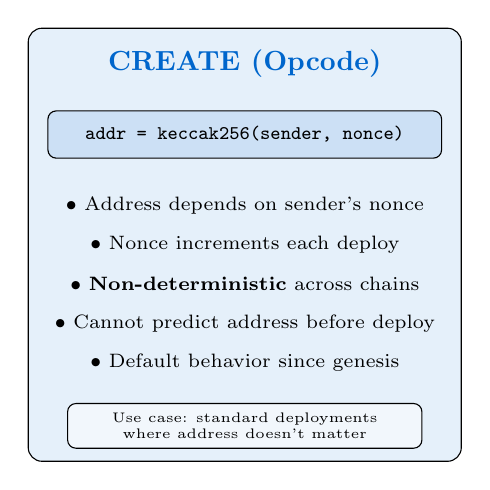
\begin{tikzpicture}[
  cbox/.style={draw,rounded corners=5pt,minimum width=5.5cm,minimum height=5.5cm,
    font=\small,align=center},
  formula/.style={draw,rounded corners=3pt,font=\scriptsize\ttfamily,
    minimum width=5cm,minimum height=0.6cm,align=center},
  feat/.style={font=\scriptsize,align=left}
]
  \node[cbox,fill=mlblue!10] (c1) at (0,0) {};
  \node[font=\normalsize\bfseries,mlblue] at (0,2.3) {CREATE (Opcode)};
  \node[formula,fill=mlblue!20] at (0,1.4) {addr = keccak256(sender, nonce)};
  \node[feat] at (0,0.5) {$\bullet$ Address depends on sender's nonce};
  \node[feat] at (0,0) {$\bullet$ Nonce increments each deploy};
  \node[feat] at (0,-0.5) {$\bullet$ \textbf{Non-deterministic} across chains};
  \node[feat] at (0,-1.0) {$\bullet$ Cannot predict address before deploy};
  \node[feat] at (0,-1.5) {$\bullet$ Default behavior since genesis};
  \node[draw,rounded corners=3pt,fill=mlblue!5,font=\tiny,align=center,
    minimum width=4.5cm] at (0,-2.3) {
    Use case: standard deployments\\where address doesn't matter
  };
\end{tikzpicture}
\end{center}
\column{0.48\textwidth}
\begin{center}
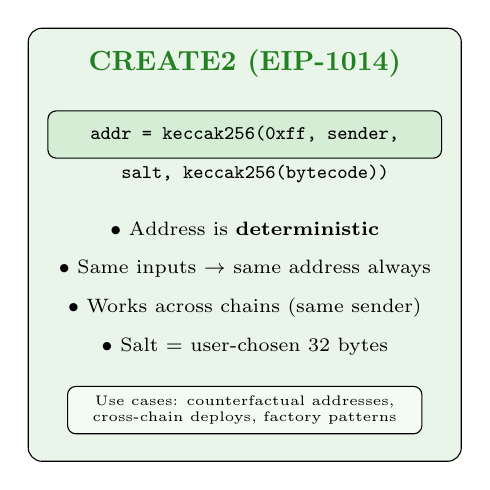
\begin{tikzpicture}[
  cbox/.style={draw,rounded corners=5pt,minimum width=5.5cm,minimum height=5.5cm,
    font=\small,align=center},
  formula/.style={draw,rounded corners=3pt,font=\scriptsize\ttfamily,
    minimum width=5cm,minimum height=0.6cm,align=center},
  feat/.style={font=\scriptsize,align=left}
]
  \node[cbox,fill=mlgreen!10] (c2) at (0,0) {};
  \node[font=\normalsize\bfseries,mlgreen!80!black] at (0,2.3) {CREATE2 (EIP-1014)};
  \node[formula,fill=mlgreen!20] at (0,1.4) {addr = keccak256(0xff, sender,};
  \node[font=\scriptsize\ttfamily,align=center] at (0,0.9) {~~salt, keccak256(bytecode))};
  \node[feat] at (0,0.2) {$\bullet$ Address is \textbf{deterministic}};
  \node[feat] at (0,-0.3) {$\bullet$ Same inputs $\to$ same address always};
  \node[feat] at (0,-0.8) {$\bullet$ Works across chains (same sender)};
  \node[feat] at (0,-1.3) {$\bullet$ Salt = user-chosen 32 bytes};
  \node[draw,rounded corners=3pt,fill=mlgreen!5,font=\tiny,align=center,
    minimum width=4.5cm] at (0,-2.1) {
    Use cases: counterfactual addresses,\\cross-chain deploys, factory patterns
  };
\end{tikzpicture}
\end{center}
\end{columns}
\vspace{3mm}
\begin{block}{Why CREATE2 Matters}
\small Deterministic addresses enable \textbf{counterfactual instantiation}: you can compute a contract's address \emph{before} deploying it, allowing users to send funds to a contract that doesn't exist yet (used in state channels, account abstraction, and cross-chain protocols).
\end{block}
\bottomnote{CREATE2 was introduced via EIP-1014 (2018) -- the \texttt{0xff} prefix prevents collision with CREATE addresses}
\end{frame}

%--- FRAME 40: Interacting with Contracts ---
\begin{frame}{Interacting with Contracts}
\begin{center}
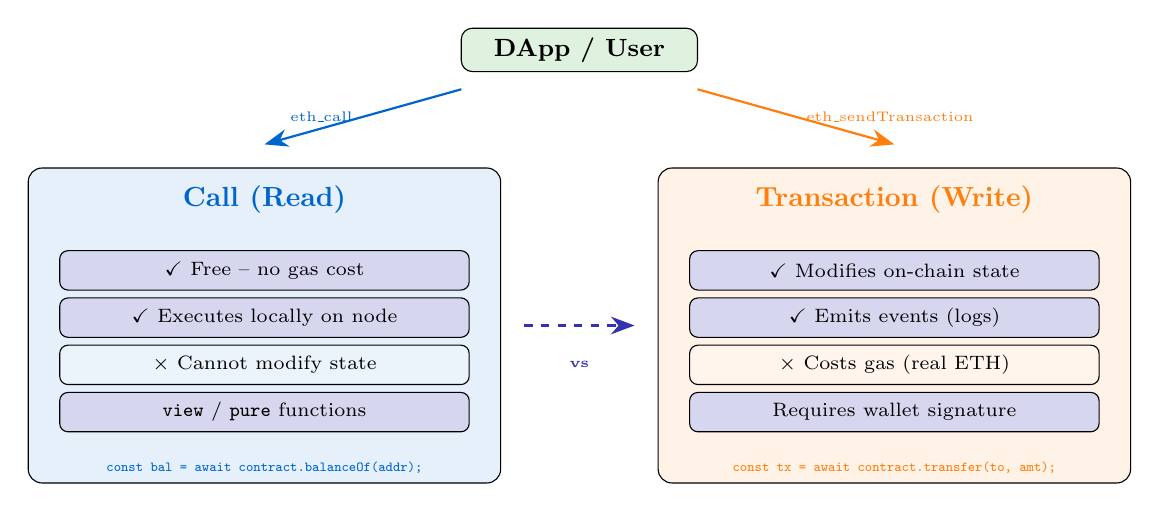
\begin{tikzpicture}[
  ibox/.style={draw,rounded corners=5pt,minimum width=6cm,minimum height=4cm,
    font=\small,align=center},
  prop/.style={draw,rounded corners=3pt,fill=mllavender4,font=\scriptsize,
    minimum width=5.2cm,minimum height=0.5cm,align=left},
  arr/.style={-{Stealth[length=3mm]},thick}
]
  % Call
  \node[ibox,fill=mlblue!10] (call) at (0,0) {};
  \node[font=\normalsize\bfseries,mlblue] at (0,1.6) {Call (Read)};
  \node[prop] at (0,0.7) {$\checkmark$ Free -- no gas cost};
  \node[prop] at (0,0.1) {$\checkmark$ Executes locally on node};
  \node[prop,fill=mlblue!8] at (0,-0.5) {$\times$ Cannot modify state};
  \node[prop] at (0,-1.1) {\texttt{view} / \texttt{pure} functions};
  \node[font=\tiny\ttfamily,mlblue,align=center] at (0,-1.8) {const bal = await contract.balanceOf(addr);};

  % Transaction
  \node[ibox,fill=mlorange!10] (txn) at (8,0) {};
  \node[font=\normalsize\bfseries,mlorange] at (8,1.6) {Transaction (Write)};
  \node[prop] at (8,0.7) {$\checkmark$ Modifies on-chain state};
  \node[prop] at (8,0.1) {$\checkmark$ Emits events (logs)};
  \node[prop,fill=mlorange!8] at (8,-0.5) {$\times$ Costs gas (real ETH)};
  \node[prop] at (8,-1.1) {Requires wallet signature};
  \node[font=\tiny\ttfamily,mlorange,align=center] at (8,-1.8) {const tx = await contract.transfer(to, amt);};

  % Comparison arrow
  \draw[arr,mlpurple,dashed] (3.3,0) -- (4.7,0);
  \node[font=\tiny\bfseries,mlpurple,align=center] at (4,-0.5) {vs};

  % User at top
  \node[draw,rounded corners=4pt,fill=mlgreen!15,font=\small\bfseries,align=center,
    minimum width=3cm] (user) at (4,3.5) {DApp / User};
  \draw[arr,mlblue] (2.5,3) -- (0,2.3) node[midway,left,font=\tiny]{eth\_call};
  \draw[arr,mlorange] (5.5,3) -- (8,2.3) node[midway,right,font=\tiny]{eth\_sendTransaction};
\end{tikzpicture}
\end{center}
\vspace{2mm}
\begin{alertblock}{Common Gotcha}
\small Calling a state-changing function with \texttt{eth\_call} will \emph{simulate} it (returning a result) but \textbf{not} persist changes. You must send a \textbf{transaction} for state to update on-chain. Conversely, calling a \texttt{view} function via transaction wastes gas.
\end{alertblock}
\bottomnote{ethers.js v6: \texttt{contract.functionName()} auto-detects call vs transaction based on the function's mutability}
\end{frame}

%--- FRAME 41: Testing Smart Contracts ---
\begin{frame}{Testing Smart Contracts}
\begin{columns}
\column{0.45\textwidth}
\begin{center}
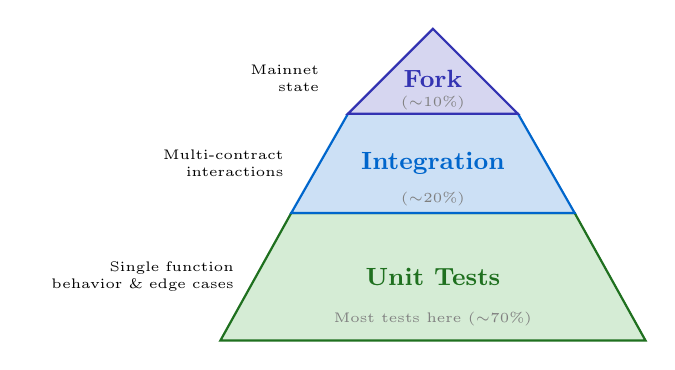
\begin{tikzpicture}[scale=0.9]
  % Pyramid
  \fill[mlgreen!20] (-3,0) -- (3,0) -- (2,1.8) -- (-2,1.8) -- cycle;
  \draw[thick,mlgreen!70!black] (-3,0) -- (3,0) -- (2,1.8) -- (-2,1.8) -- cycle;
  \node[font=\small\bfseries,mlgreen!70!black,align=center] at (0,0.9) {Unit Tests};
  \node[font=\tiny,mlgray] at (0,0.3) {Most tests here ($\sim$70\%)};

  \fill[mlblue!20] (-2,1.8) -- (2,1.8) -- (1.2,3.2) -- (-1.2,3.2) -- cycle;
  \draw[thick,mlblue] (-2,1.8) -- (2,1.8) -- (1.2,3.2) -- (-1.2,3.2) -- cycle;
  \node[font=\small\bfseries,mlblue,align=center] at (0,2.5) {Integration};
  \node[font=\tiny,mlgray] at (0,2.0) {($\sim$20\%)};

  \fill[mlpurple!20] (-1.2,3.2) -- (1.2,3.2) -- (0,4.4) -- cycle;
  \draw[thick,mlpurple] (-1.2,3.2) -- (1.2,3.2) -- (0,4.4) -- cycle;
  \node[font=\small\bfseries,mlpurple,align=center] at (0,3.7) {Fork};
  \node[font=\tiny,mlgray] at (0,3.35) {($\sim$10\%)};

  % Labels
  \node[font=\tiny,align=right,text width=2.5cm] at (-4.2,0.9) {Single function\\behavior \& edge cases};
  \node[font=\tiny,align=right,text width=2.5cm] at (-3.5,2.5) {Multi-contract\\interactions};
  \node[font=\tiny,align=right,text width=2.5cm] at (-3,3.7) {Mainnet\\state};
\end{tikzpicture}
\end{center}
\column{0.52\textwidth}
\begin{block}{Testing Frameworks}
\small
\begin{tabular}{@{}lll@{}}
\toprule
\textbf{Tool} & \textbf{Language} & \textbf{Speed} \\
\midrule
Foundry & Solidity & Very fast \\
Hardhat & JS/TS & Moderate \\
Brownie & Python & Moderate \\
\bottomrule
\end{tabular}
\end{block}
\vspace{1mm}
\begin{block}{Key Testing Techniques}
\begin{itemize}\small
  \item \textbf{Fuzzing}: random inputs find edge cases
  \item \textbf{Invariant testing}: properties that must always hold
  \item \textbf{Fork testing}: replay against real mainnet state
  \item \textbf{Gas snapshots}: detect regressions
\end{itemize}
\end{block}
\vspace{1mm}
\begin{alertblock}{Coverage Target}
\small Aim for $>$95\% line coverage. Critical paths (fund transfers, access control) must have 100\% branch coverage.
\end{alertblock}
\end{columns}
\bottomnote{``Code without tests is broken by design'' -- a \$100M contract with 50\% coverage is an audit red flag}
\end{frame}

%--- FRAME 42: Security Vulnerabilities ---
\begin{frame}{Security Vulnerabilities}
\begin{center}
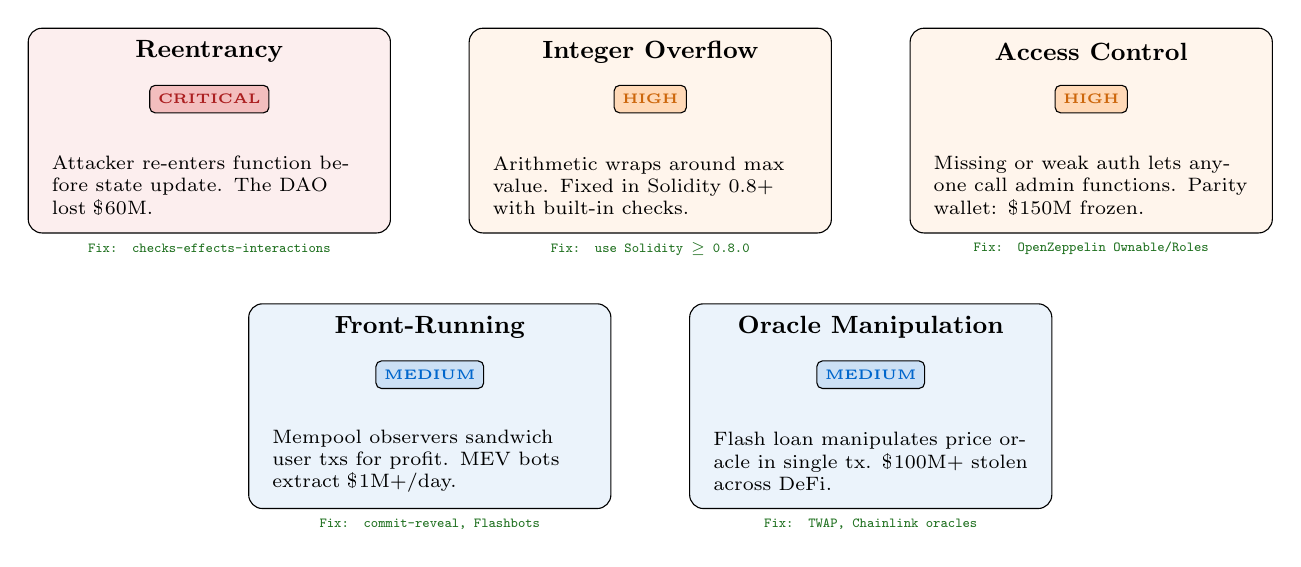
\begin{tikzpicture}[
  vulncard/.style={draw,rounded corners=5pt,minimum width=4.6cm,minimum height=2.6cm,
    font=\small,align=center},
  sevbadge/.style={draw,rounded corners=2pt,font=\tiny\bfseries,inner sep=3pt,
    minimum height=0.35cm},
  desc/.style={font=\scriptsize,align=left,text width=4cm}
]
  % Row 1
  % Reentrancy
  \node[vulncard,fill=mlred!8] (v1) at (0,2) {};
  \node[font=\small\bfseries] at (0,3) {Reentrancy};
  \node[sevbadge,fill=mlred!30,text=mlred!80!black] at (0,2.4) {CRITICAL};
  \node[desc] at (0,1.3) {Attacker re-enters function before state update. The DAO lost \$60M.};
  \node[font=\tiny\ttfamily,mlgreen!70!black] at (0,0.5) {Fix: checks-effects-interactions};

  % Integer Overflow
  \node[vulncard,fill=mlorange!8] (v2) at (5.6,2) {};
  \node[font=\small\bfseries] at (5.6,3) {Integer Overflow};
  \node[sevbadge,fill=mlorange!30,text=mlorange!80!black] at (5.6,2.4) {HIGH};
  \node[desc] at (5.6,1.3) {Arithmetic wraps around max value. Fixed in Solidity 0.8+ with built-in checks.};
  \node[font=\tiny\ttfamily,mlgreen!70!black] at (5.6,0.5) {Fix: use Solidity $\geq$ 0.8.0};

  % Access Control
  \node[vulncard,fill=mlorange!8] (v3) at (11.2,2) {};
  \node[font=\small\bfseries] at (11.2,3) {Access Control};
  \node[sevbadge,fill=mlorange!30,text=mlorange!80!black] at (11.2,2.4) {HIGH};
  \node[desc] at (11.2,1.3) {Missing or weak auth lets anyone call admin functions. Parity wallet: \$150M frozen.};
  \node[font=\tiny\ttfamily,mlgreen!70!black] at (11.2,0.5) {Fix: OpenZeppelin Ownable/Roles};

  % Row 2
  % Front-running
  \node[vulncard,fill=mlblue!8] (v4) at (2.8,-1.5) {};
  \node[font=\small\bfseries] at (2.8,-0.5) {Front-Running};
  \node[sevbadge,fill=mlblue!20,text=mlblue] at (2.8,-1.1) {MEDIUM};
  \node[desc] at (2.8,-2.2) {Mempool observers sandwich user txs for profit. MEV bots extract \$1M+/day.};
  \node[font=\tiny\ttfamily,mlgreen!70!black] at (2.8,-3.0) {Fix: commit-reveal, Flashbots};

  % Oracle Manipulation
  \node[vulncard,fill=mlblue!8] (v5) at (8.4,-1.5) {};
  \node[font=\small\bfseries] at (8.4,-0.5) {Oracle Manipulation};
  \node[sevbadge,fill=mlblue!20,text=mlblue] at (8.4,-1.1) {MEDIUM};
  \node[desc] at (8.4,-2.2) {Flash loan manipulates price oracle in single tx. \$100M+ stolen across DeFi.};
  \node[font=\tiny\ttfamily,mlgreen!70!black] at (8.4,-3.0) {Fix: TWAP, Chainlink oracles};
\end{tikzpicture}
\end{center}
\bottomnote{Smart contract vulnerabilities have caused $>$\$5B in losses -- security is not optional, it is existential}
\end{frame}

%--- FRAME 43: The DAO Hack Case Study ---
\begin{frame}{The DAO Hack Case Study}
\begin{center}
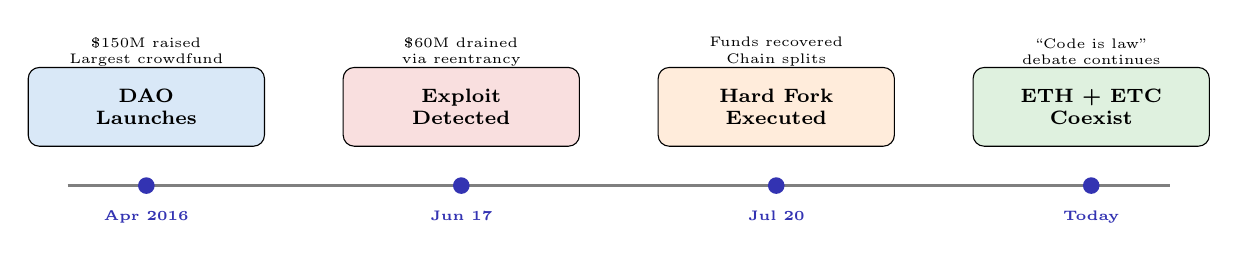
\begin{tikzpicture}[
  event/.style={draw,rounded corners=4pt,minimum width=3cm,minimum height=1cm,
    font=\scriptsize\bfseries,align=center},
  arr/.style={-{Stealth[length=3mm]},thick,mlpurple},
  note/.style={font=\tiny,align=center}
]
  % Timeline
  \draw[thick,mlgray] (0,3.5) -- (14,3.5);
  \foreach \x/\label in {1/Apr 2016, 5/Jun 17, 9/Jul 20, 13/Today} {
    \fill[mlpurple] (\x,3.5) circle(3pt);
    \node[font=\tiny\bfseries,mlpurple,below] at (\x,3.3) {\label};
  }

  \node[event,fill=mlblue!15] at (1,4.5) {DAO\\Launches};
  \node[note] at (1,5.2) {\$150M raised\\Largest crowdfund};

  \node[event,fill=mlred!15] at (5,4.5) {Exploit\\Detected};
  \node[note] at (5,5.2) {\$60M drained\\via reentrancy};

  \node[event,fill=mlorange!15] at (9,4.5) {Hard Fork\\Executed};
  \node[note] at (9,5.2) {Funds recovered\\Chain splits};

  \node[event,fill=mlgreen!15] at (13,4.5) {ETH + ETC\\Coexist};
  \node[note] at (13,5.2) {``Code is law''\\debate continues};
\end{tikzpicture}
\end{center}
\vspace{1mm}
\begin{center}
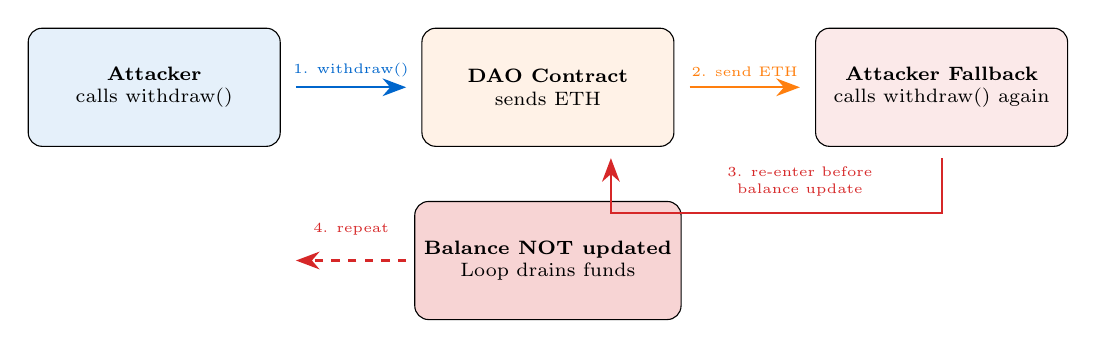
\begin{tikzpicture}[
  rbox/.style={draw,rounded corners=5pt,minimum width=3.2cm,minimum height=1.5cm,
    font=\scriptsize,align=center},
  arr/.style={-{Stealth[length=3mm]},thick}
]
  % Reentrancy flow
  \node[rbox,fill=mlblue!10] (attacker) at (0,0) {\textbf{Attacker}\\calls withdraw()};
  \node[rbox,fill=mlorange!10] (dao) at (5,0) {\textbf{DAO Contract}\\sends ETH};
  \node[rbox,fill=mlred!10] (fallback) at (10,0) {\textbf{Attacker Fallback}\\calls withdraw() again};
  \node[rbox,fill=mlred!20] (drain) at (5,-2.2) {\textbf{Balance NOT updated}\\Loop drains funds};

  \draw[arr,mlblue] (1.8,0) -- (3.2,0) node[midway,above,font=\tiny]{1. withdraw()};
  \draw[arr,mlorange] (6.8,0) -- (8.2,0) node[midway,above,font=\tiny]{2. send ETH};
  \draw[arr,mlred] (10,-.9) -- (10,-1.6) -- (5.8,-1.6) -- (5.8,-0.9);
  \node[font=\tiny,mlred,align=center] at (8.2,-1.2) {3. re-enter before\\balance update};
  \draw[arr,mlred,dashed] (3.2,-2.2) -- (1.8,-2.2);
  \node[font=\tiny,mlred] at (2.5,-1.8) {4. repeat};
\end{tikzpicture}
\end{center}
\vspace{1mm}
\begin{block}{The Fix: Checks-Effects-Interactions Pattern}
\small \textbf{1.} Check conditions (require) $\to$ \textbf{2.} Update state (set balance to 0) $\to$ \textbf{3.} External call (send ETH). Never call external contracts before updating your own state.
\end{block}
\bottomnote{The DAO hack led to the Ethereum/Ethereum Classic split and fundamentally shaped smart contract security practices}
\end{frame}

%--- FRAME 44: Upgradeability Patterns ---
\begin{frame}{Upgradeability Patterns}
\begin{center}
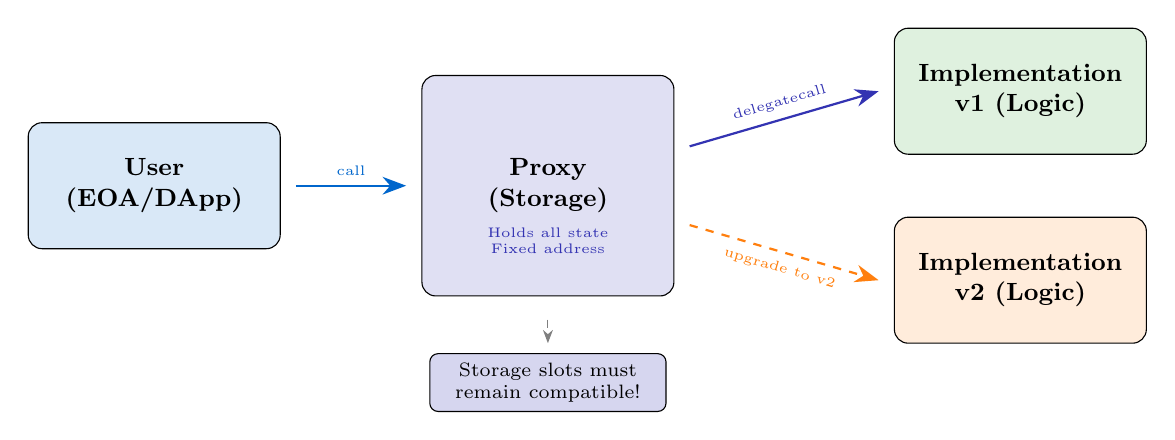
\begin{tikzpicture}[
  comp/.style={draw,rounded corners=5pt,minimum width=3.2cm,minimum height=1.6cm,
    font=\small\bfseries,align=center},
  arr/.style={-{Stealth[length=3mm]},thick},
  note/.style={font=\tiny,align=center}
]
  % Proxy Pattern Diagram
  \node[comp,fill=mlblue!15] (user) at (0,0) {User\\(EOA/DApp)};
  \node[comp,fill=mlpurple!15,minimum height=2.8cm] (proxy) at (5,0) {Proxy\\(Storage)};
  \node[font=\tiny,mlpurple,align=center] at (5,-0.7) {Holds all state\\Fixed address};
  \node[comp,fill=mlgreen!15] (implv1) at (11,1.2) {Implementation\\v1 (Logic)};
  \node[comp,fill=mlorange!15] (implv2) at (11,-1.2) {Implementation\\v2 (Logic)};

  \draw[arr,mlblue] (1.8,0) -- (3.2,0) node[midway,above,font=\tiny]{call};
  \draw[arr,mlpurple] (6.8,0.5) -- (9.2,1.2) node[midway,above,font=\tiny,sloped]{delegatecall};
  \draw[arr,mlorange,dashed] (6.8,-0.5) -- (9.2,-1.2) node[midway,below,font=\tiny,sloped]{upgrade to v2};

  % Storage note
  \node[draw,rounded corners=3pt,fill=mllavender4,font=\scriptsize,align=center,
    minimum width=3cm] at (5,-2.5) {Storage slots must\\remain compatible!};
  \draw[-{Stealth},mlgray,dashed] (5,-1.7) -- (5,-2);
\end{tikzpicture}
\end{center}
\vspace{2mm}
\begin{columns}
\column{0.48\textwidth}
\begin{block}{Transparent Proxy (TPP)}
\begin{itemize}\small
  \item Admin calls $\to$ proxy logic (upgrade)
  \item User calls $\to$ delegatecall to implementation
  \item Clear separation of concerns
  \item Higher gas: admin check on every call
\end{itemize}
\end{block}
\column{0.48\textwidth}
\begin{block}{UUPS (EIP-1822)}
\begin{itemize}\small
  \item Upgrade logic lives in \emph{implementation}
  \item Proxy is minimal (cheaper deploys)
  \item Implementation must include upgrade function
  \item Risk: forgetting upgrade function = bricked
\end{itemize}
\end{block}
\end{columns}
\vspace{2mm}
\begin{alertblock}{Storage Collision Warning}
\small Both patterns use \texttt{delegatecall}: the implementation's code runs in the proxy's storage context. Storage slot layout \textbf{must} be append-only between versions -- reordering or removing variables corrupts state.
\end{alertblock}
\bottomnote{EIP-1967 standardizes storage slots for proxy admin and implementation address to prevent collisions}
\end{frame}

%--- FRAME 45: Contract Verification & Etherscan ---
\begin{frame}{Contract Verification \& Etherscan}
\begin{center}
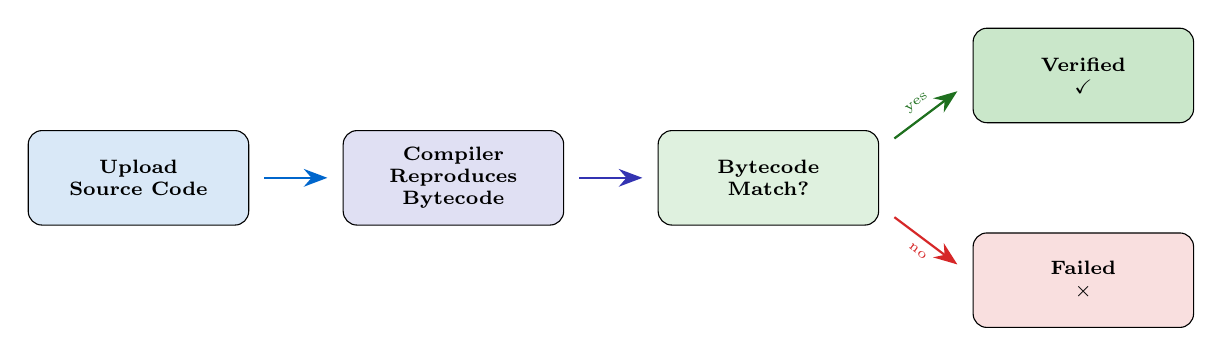
\begin{tikzpicture}[
  procbox/.style={draw,rounded corners=5pt,minimum width=2.8cm,minimum height=1.2cm,
    font=\scriptsize\bfseries,align=center},
  arr/.style={-{Stealth[length=3mm]},thick},
  note/.style={font=\tiny,align=center}
]
  % Verification flow
  \node[procbox,fill=mlblue!15] (src) at (0,1.5) {Upload\\Source Code};
  \node[procbox,fill=mlpurple!15] (compile) at (4,1.5) {Compiler\\Reproduces\\Bytecode};
  \node[procbox,fill=mlgreen!15] (match) at (8,1.5) {Bytecode\\Match?};
  \node[procbox,fill=mlgreen!25] (yes) at (12,2.8) {Verified\\$\checkmark$};
  \node[procbox,fill=mlred!15] (no) at (12,0.2) {Failed\\$\times$};

  \draw[arr,mlblue] (1.6,1.5) -- (2.4,1.5);
  \draw[arr,mlpurple] (5.6,1.5) -- (6.4,1.5);
  \draw[arr,mlgreen!70!black] (9.6,2) -- (10.4,2.6) node[midway,above,font=\tiny,sloped]{yes};
  \draw[arr,mlred] (9.6,1) -- (10.4,0.4) node[midway,below,font=\tiny,sloped]{no};
\end{tikzpicture}
\end{center}
\vspace{2mm}
\begin{columns}
\column{0.48\textwidth}
\begin{block}{Verified Contract}
\colorbox{mlgreen!10}{\parbox{0.92\linewidth}{\small
\textbf{$\checkmark$ Green checkmark on Etherscan}\\[1mm]
$\bullet$ Source code readable by anyone\\
$\bullet$ Read/Write contract UI available\\
$\bullet$ Function names visible in tx decoder\\
$\bullet$ Users can audit the logic
}}
\end{block}
\column{0.48\textwidth}
\begin{block}{Unverified Contract}
\colorbox{mlred!10}{\parbox{0.92\linewidth}{\small
\textbf{$\times$ No source code visible}\\[1mm]
$\bullet$ Only raw hex bytecode shown\\
$\bullet$ Function calls show as hex selectors\\
$\bullet$ Cannot easily audit logic\\
$\bullet$ \textbf{Major trust red flag}
}}
\end{block}
\end{columns}
\vspace{2mm}
\begin{alertblock}{Verification Methods}
\small \textbf{Flatten}: combine all files into one $\to$ upload. \textbf{Standard JSON}: compiler input JSON (preserves imports). \textbf{Hardhat/Foundry plugins}: \texttt{hardhat verify} or \texttt{forge verify-contract} -- automates the process.
\end{alertblock}
\bottomnote{Always verify your contracts -- unverified contracts receive significantly less trust and TVL from the DeFi community}
\end{frame}

%--- FRAME 46: Deploy Section Summary ---
\begin{frame}{Deploy \& Interact: Section Summary}
\begin{columns}
\column{0.48\textwidth}
\begin{block}{Deployment Checklist}
\colorbox{mlgreen!10}{\parbox{0.92\linewidth}{\small
\begin{enumerate}
  \item[$\checkmark$] \textbf{Compile}: \texttt{solc} or framework CLI
  \item[$\checkmark$] \textbf{Test}: unit, integration, fork, fuzz
  \item[$\checkmark$] \textbf{Audit}: internal review + external firm
  \item[$\checkmark$] \textbf{Deploy}: testnet first, then mainnet
  \item[$\checkmark$] \textbf{Verify}: source code on Etherscan
  \item[$\checkmark$] \textbf{Monitor}: events, alerts, dashboards
\end{enumerate}
}}
\end{block}
\vspace{1mm}
\begin{block}{Key Tools}
\colorbox{mlblue!10}{\parbox{0.92\linewidth}{\small
\textbf{Frameworks}: Hardhat, Foundry, Remix\\
\textbf{Testing}: Forge, Echidna, Mythril\\
\textbf{Deploy}: Hardhat Ignition, forge create\\
\textbf{Monitor}: Tenderly, OpenZeppelin Defender\\
\textbf{Verify}: Etherscan, Sourcify
}}
\end{block}
\column{0.48\textwidth}
\begin{block}{Security Essentials}
\colorbox{mlred!10}{\parbox{0.92\linewidth}{\small
\textbf{Top vulnerabilities}:\\
$\bullet$ Reentrancy (checks-effects-interactions)\\
$\bullet$ Access control (role-based auth)\\
$\bullet$ Oracle manipulation (TWAP + Chainlink)\\
$\bullet$ Front-running (commit-reveal, Flashbots)\\[2mm]
\textbf{Patterns that protect}:\\
$\bullet$ OpenZeppelin libraries\\
$\bullet$ Proxy patterns for upgradeability\\
$\bullet$ Timelocks for governance\\
$\bullet$ Circuit breakers (Pausable)
}}
\end{block}
\vspace{1mm}
\begin{alertblock}{Golden Rule}
\small Immutable code + real money = \textbf{zero room for error}. Every deployed contract should be tested, audited, and verified before holding user funds.
\end{alertblock}
\end{columns}
\bottomnote{Next section: Summary, token standards, DeFi building blocks, and the full-stack DApp architecture}
\end{frame}

\section{Summary and Integration}

%--- FRAME 47: Full Stack DApp Architecture ---
\begin{frame}{Full Stack DApp Architecture}
\begin{center}
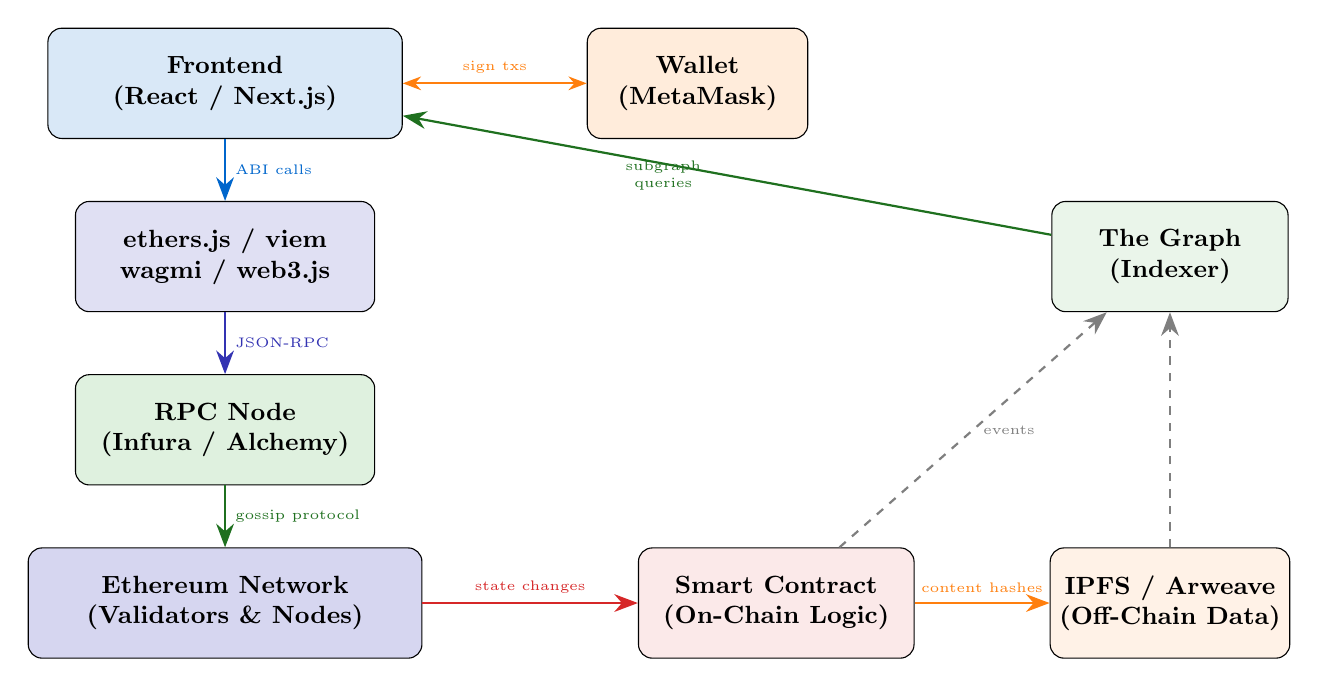
\begin{tikzpicture}[
  layer/.style={draw,rounded corners=5pt,minimum height=1.4cm,font=\small\bfseries,align=center},
  arr/.style={-{Stealth[length=3mm]},thick},
  lbl/.style={font=\tiny,align=center}
]
  % Frontend
  \node[layer,fill=mlblue!15,minimum width=4.5cm] (fe) at (0,3) {Frontend\\(React / Next.js)};

  % Web3 Library
  \node[layer,fill=mlpurple!15,minimum width=3.8cm] (lib) at (0,0.8) {ethers.js / viem\\wagmi / web3.js};

  % Wallet
  \node[layer,fill=mlorange!15,minimum width=2.8cm] (wallet) at (6,3) {Wallet\\(MetaMask)};

  % RPC Node
  \node[layer,fill=mlgreen!15,minimum width=3.8cm] (rpc) at (0,-1.4) {RPC Node\\(Infura / Alchemy)};

  % Ethereum
  \node[layer,fill=mlpurple!20,minimum width=5cm] (eth) at (0,-3.6) {Ethereum Network\\(Validators \& Nodes)};

  % Smart Contract
  \node[layer,fill=mlred!10,minimum width=3.5cm] (sc) at (7,-3.6) {Smart Contract\\(On-Chain Logic)};

  % IPFS
  \node[layer,fill=mlorange!10,minimum width=3cm] (ipfs) at (12,-3.6) {IPFS / Arweave\\(Off-Chain Data)};

  % The Graph
  \node[layer,fill=mlgreen!10,minimum width=3cm] (graph) at (12,0.8) {The Graph\\(Indexer)};

  % Arrows with labels
  \draw[arr,mlblue] (fe) -- (lib) node[midway,right,lbl]{ABI calls};
  \draw[arr,mlpurple] (lib) -- (rpc) node[midway,right,lbl]{JSON-RPC};
  \draw[arr,mlgreen!70!black] (rpc) -- (eth) node[midway,right,lbl]{gossip protocol};
  \draw[arr,mlred] (eth) -- (sc) node[midway,above,lbl]{state changes};
  \draw[arr,mlorange] (sc) -- (ipfs) node[midway,above,lbl]{content hashes};
  \draw[{Stealth}-{Stealth},thick,mlorange] (fe) -- (wallet) node[midway,above,lbl]{sign txs};
  \draw[arr,mlgreen!70!black] (graph) -- (fe) node[midway,left,lbl,xshift=-2mm]{subgraph\\queries};
  \draw[arr,mlgray,dashed] (sc) -- (graph) node[midway,right,lbl]{events};
  \draw[arr,mlgray,dashed] (ipfs) -- (graph);
\end{tikzpicture}
\end{center}
\vspace{1mm}
\begin{alertblock}{Decentralization Spectrum}
\small Most ``DApps'' centralize the frontend (hosted on Vercel/AWS). True decentralization requires: frontend on IPFS, ENS for naming, The Graph for indexing, and the smart contract for logic -- no single point of failure.
\end{alertblock}
\bottomnote{A fully decentralized DApp has no admin keys, no centralized hosting, and no off-chain dependencies that can be censored}
\end{frame}

%--- FRAME 48: Token Standards Overview ---
\begin{frame}{Token Standards Overview}
\begin{center}
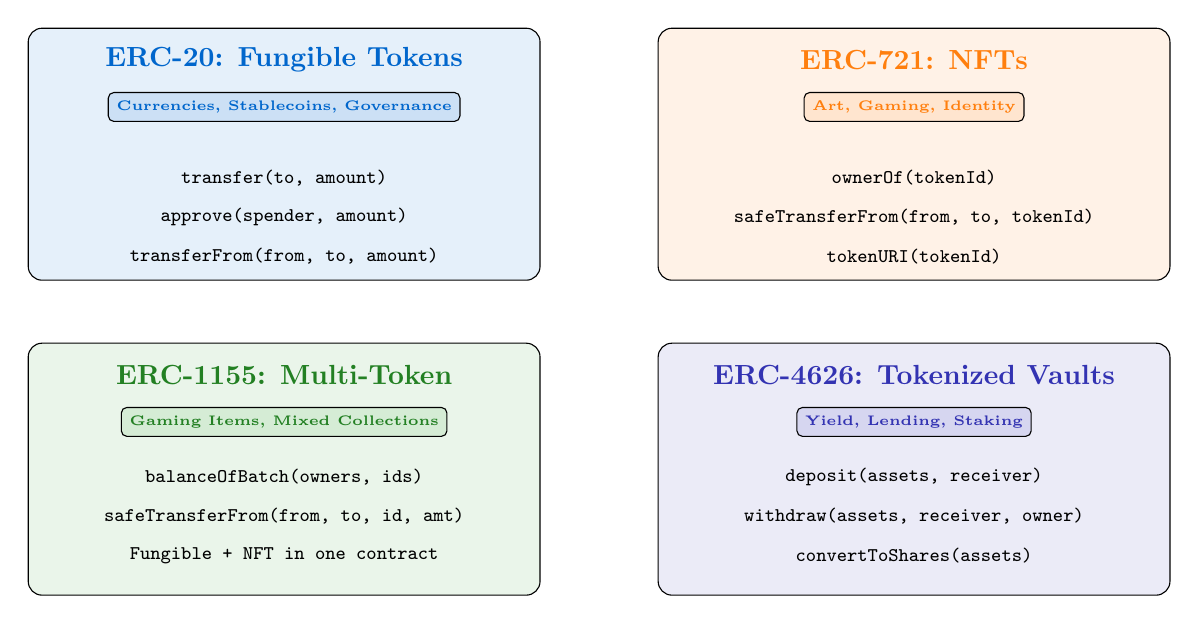
\begin{tikzpicture}[
  tcard/.style={draw,rounded corners=5pt,minimum width=6.5cm,minimum height=3.2cm,
    font=\small,align=center},
  func/.style={font=\scriptsize\ttfamily,align=left},
  badge/.style={draw,rounded corners=2pt,font=\tiny\bfseries,inner sep=3pt}
]
  % ERC-20
  \node[tcard,fill=mlblue!10] (e20) at (0,2.5) {};
  \node[font=\normalsize\bfseries,mlblue] at (0,3.7) {ERC-20: Fungible Tokens};
  \node[badge,fill=mlblue!20,text=mlblue] at (0,3.1) {Currencies, Stablecoins, Governance};
  \node[func] at (0,2.2) {transfer(to, amount)};
  \node[func] at (0,1.7) {approve(spender, amount)};
  \node[func] at (0,1.2) {transferFrom(from, to, amount)};

  % ERC-721
  \node[tcard,fill=mlorange!10] (e721) at (8,2.5) {};
  \node[font=\normalsize\bfseries,mlorange] at (8,3.7) {ERC-721: NFTs};
  \node[badge,fill=mlorange!20,text=mlorange] at (8,3.1) {Art, Gaming, Identity};
  \node[func] at (8,2.2) {ownerOf(tokenId)};
  \node[func] at (8,1.7) {safeTransferFrom(from, to, tokenId)};
  \node[func] at (8,1.2) {tokenURI(tokenId)};

  % ERC-1155
  \node[tcard,fill=mlgreen!10] (e1155) at (0,-1.5) {};
  \node[font=\normalsize\bfseries,mlgreen!80!black] at (0,-0.3) {ERC-1155: Multi-Token};
  \node[badge,fill=mlgreen!20,text=mlgreen!80!black] at (0,-0.9) {Gaming Items, Mixed Collections};
  \node[func] at (0,-1.6) {balanceOfBatch(owners, ids)};
  \node[func] at (0,-2.1) {safeTransferFrom(from, to, id, amt)};
  \node[func] at (0,-2.6) {Fungible + NFT in one contract};

  % ERC-4626
  \node[tcard,fill=mlpurple!10] (e4626) at (8,-1.5) {};
  \node[font=\normalsize\bfseries,mlpurple] at (8,-0.3) {ERC-4626: Tokenized Vaults};
  \node[badge,fill=mlpurple!20,text=mlpurple] at (8,-0.9) {Yield, Lending, Staking};
  \node[func] at (8,-1.6) {deposit(assets, receiver)};
  \node[func] at (8,-2.1) {withdraw(assets, receiver, owner)};
  \node[func] at (8,-2.6) {convertToShares(assets)};
\end{tikzpicture}
\end{center}
\bottomnote{Token standards are interfaces (ERCs) -- they define \emph{what} functions exist, not \emph{how} they work internally}
\end{frame}

%--- FRAME 49: DeFi Building Blocks ---
\begin{frame}{DeFi Building Blocks}
\begin{columns}
\column{0.5\textwidth}
\begin{center}
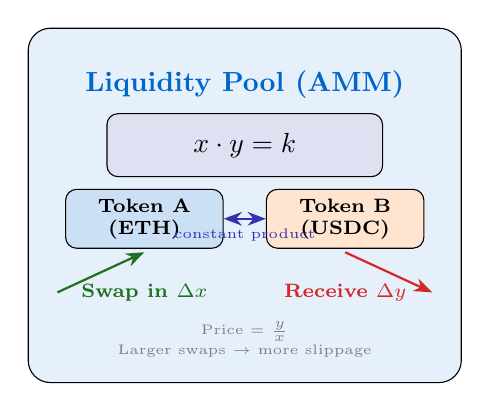
\begin{tikzpicture}[scale=0.85]
  % AMM Pool
  \node[draw,rounded corners=8pt,fill=mlblue!10,minimum width=5.5cm,minimum height=4.5cm] (pool) at (0,0) {};
  \node[font=\normalsize\bfseries,mlblue] at (0,1.8) {Liquidity Pool (AMM)};

  % Formula
  \node[draw,rounded corners=4pt,fill=mlpurple!15,font=\normalsize,
    minimum width=3.5cm,minimum height=0.8cm] at (0,0.9) {$x \cdot y = k$};

  % Token balances
  \node[draw,rounded corners=4pt,fill=mlblue!20,font=\scriptsize\bfseries,
    minimum width=2cm,minimum height=0.7cm,align=center] (tokA) at (-1.5,-0.2) {Token A\\(ETH)};
  \node[draw,rounded corners=4pt,fill=mlorange!20,font=\scriptsize\bfseries,
    minimum width=2cm,minimum height=0.7cm,align=center] (tokB) at (1.5,-0.2) {Token B\\(USDC)};

  \draw[{Stealth}-{Stealth},thick,mlpurple] (tokA) -- (tokB)
    node[midway,below,font=\tiny]{constant product};

  % Swap arrows
  \node[font=\scriptsize\bfseries,mlgreen!70!black] at (-1.5,-1.3) {Swap in $\Delta x$};
  \node[font=\scriptsize\bfseries,mlred] at (1.5,-1.3) {Receive $\Delta y$};
  \draw[-{Stealth},thick,mlgreen!70!black] (-2.8,-1.3) -- (-1.5,-0.7);
  \draw[-{Stealth},thick,mlred] (1.5,-0.7) -- (2.8,-1.3);

  % Price impact note
  \node[font=\tiny,mlgray,align=center] at (0,-2) {Price = $\frac{y}{x}$\\Larger swaps $\to$ more slippage};
\end{tikzpicture}
\end{center}
\column{0.47\textwidth}
\begin{block}{Money Legos: Composability}
\begin{center}
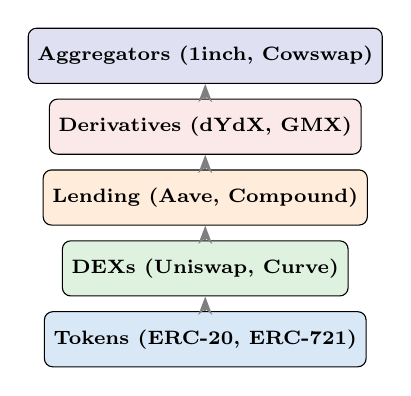
\begin{tikzpicture}[
  lego/.style={draw,rounded corners=3pt,minimum width=3.5cm,minimum height=0.7cm,
    font=\scriptsize\bfseries,align=center}
]
  \node[lego,fill=mlpurple!15] (l5) at (0,3) {Aggregators (1inch, Cowswap)};
  \node[lego,fill=mlred!10] (l4) at (0,2.1) {Derivatives (dYdX, GMX)};
  \node[lego,fill=mlorange!15] (l3) at (0,1.2) {Lending (Aave, Compound)};
  \node[lego,fill=mlgreen!15] (l2) at (0,0.3) {DEXs (Uniswap, Curve)};
  \node[lego,fill=mlblue!15] (l1) at (0,-0.6) {Tokens (ERC-20, ERC-721)};
  % Arrows
  \foreach \a/\b in {l1/l2, l2/l3, l3/l4, l4/l5} {
    \draw[-{Stealth},thick,mlgray] (\a) -- (\b);
  }
\end{tikzpicture}
\end{center}
\end{block}
\vspace{1mm}
\begin{alertblock}{Flash Loans}
\small Borrow \emph{any amount} with zero collateral -- must repay in the \textbf{same transaction}. Enables arbitrage, liquidations, and collateral swaps atomically.
\end{alertblock}
\end{columns}
\bottomnote{DeFi's composability means protocols can be combined permissionlessly -- a single tx can touch 5+ protocols}
\end{frame}

%--- FRAME 50: Ethereum Scaling Roadmap ---
\begin{frame}{Ethereum Scaling Roadmap}
\begin{center}
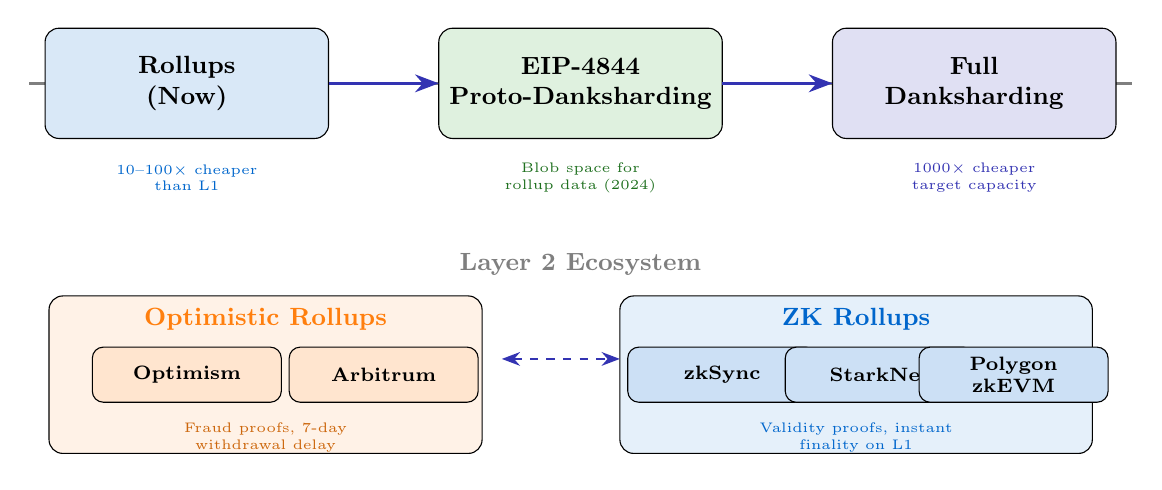
\begin{tikzpicture}[
  era/.style={draw,rounded corners=5pt,minimum width=3.6cm,minimum height=1.4cm,
    font=\small\bfseries,align=center},
  arr/.style={-{Stealth[length=3mm]},very thick,mlpurple},
  l2card/.style={draw,rounded corners=4pt,minimum width=2.4cm,minimum height=0.7cm,
    font=\scriptsize\bfseries,align=center}
]
  % Timeline
  \draw[very thick,mlgray] (0,3.5) -- (14,3.5);

  \node[era,fill=mlblue!15] (now) at (2,3.5) {Rollups\\(Now)};
  \node[era,fill=mlgreen!15] (proto) at (7,3.5) {EIP-4844\\Proto-Danksharding};
  \node[era,fill=mlpurple!15] (full) at (12,3.5) {Full\\Danksharding};

  \draw[arr] (3.8,3.5) -- (5.2,3.5);
  \draw[arr] (8.8,3.5) -- (10.2,3.5);

  % Annotations
  \node[font=\tiny,mlblue,align=center] at (2,2.3) {10--100$\times$ cheaper\\than L1};
  \node[font=\tiny,mlgreen!70!black,align=center] at (7,2.3) {Blob space for\\rollup data (2024)};
  \node[font=\tiny,mlpurple,align=center] at (12,2.3) {1000$\times$ cheaper\\target capacity};

  % L2 Ecosystem
  \node[font=\small\bfseries,mlgray] at (7,1.2) {Layer 2 Ecosystem};

  % Optimistic
  \node[draw,rounded corners=5pt,fill=mlorange!10,minimum width=5.5cm,minimum height=2cm,
    align=center] (opt) at (3,-.2) {};
  \node[font=\small\bfseries,mlorange] at (3,0.5) {Optimistic Rollups};
  \node[l2card,fill=mlorange!20] at (2,-0.2) {Optimism};
  \node[l2card,fill=mlorange!20] at (4.5,-0.2) {Arbitrum};
  \node[font=\tiny,mlorange!80!black,align=center] at (3,-1) {Fraud proofs, 7-day\\withdrawal delay};

  % ZK
  \node[draw,rounded corners=5pt,fill=mlblue!10,minimum width=6cm,minimum height=2cm,
    align=center] (zk) at (10.5,-.2) {};
  \node[font=\small\bfseries,mlblue] at (10.5,0.5) {ZK Rollups};
  \node[l2card,fill=mlblue!20] at (8.8,-0.2) {zkSync};
  \node[l2card,fill=mlblue!20] at (10.8,-0.2) {StarkNet};
  \node[l2card,fill=mlblue!20] at (12.5,-0.2) {Polygon\\zkEVM};
  \node[font=\tiny,mlblue,align=center] at (10.5,-1) {Validity proofs, instant\\finality on L1};

  % Comparison
  \draw[{Stealth}-{Stealth},thick,mlpurple,dashed] (6,0) -- (7.5,0);
\end{tikzpicture}
\end{center}
\vspace{1mm}
\begin{alertblock}{The Rollup-Centric Roadmap}
\small Ethereum L1 focuses on \textbf{security and data availability}. Execution moves to L2 rollups that inherit L1 security. EIP-4844 introduced ``blobs'' -- dedicated cheap data space for rollups, reducing L2 fees by 10--100$\times$.
\end{alertblock}
\bottomnote{As of 2024, Ethereum L2s process more transactions than L1 -- the rollup-centric roadmap is working}
\end{frame}

%--- FRAME 51: Cross-Chain & Bridges ---
\begin{frame}{Cross-Chain \& Bridges}
\begin{center}
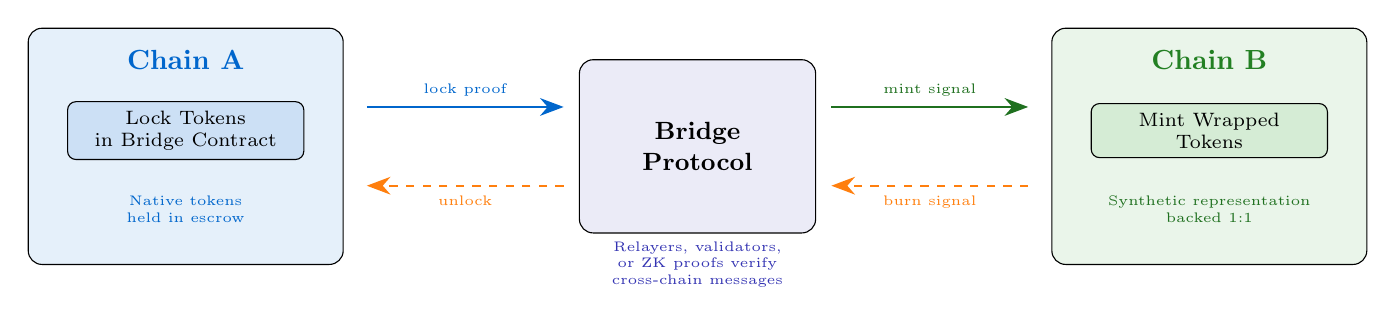
\begin{tikzpicture}[
  chain/.style={draw,rounded corners=5pt,minimum width=4cm,minimum height=3cm,
    font=\small,align=center},
  bridgebox/.style={draw,rounded corners=5pt,fill=mlpurple!10,minimum width=3cm,
    minimum height=2.2cm,font=\small\bfseries,align=center},
  arr/.style={-{Stealth[length=3mm]},thick},
  note/.style={font=\tiny,align=center}
]
  % Chain A
  \node[chain,fill=mlblue!10] (chainA) at (0,0) {};
  \node[font=\normalsize\bfseries,mlblue] at (0,1.1) {Chain A};
  \node[draw,rounded corners=3pt,fill=mlblue!20,font=\scriptsize,align=center,
    minimum width=3cm] at (0,0.2) {Lock Tokens\\in Bridge Contract};
  \node[note,mlblue] at (0,-0.8) {Native tokens\\held in escrow};

  % Bridge
  \node[bridgebox] (bridge) at (6.5,0) {Bridge\\Protocol};
  \node[note,mlpurple] at (6.5,-1.5) {Relayers, validators,\\or ZK proofs verify\\cross-chain messages};

  % Chain B
  \node[chain,fill=mlgreen!10] (chainB) at (13,0) {};
  \node[font=\normalsize\bfseries,mlgreen!80!black] at (13,1.1) {Chain B};
  \node[draw,rounded corners=3pt,fill=mlgreen!20,font=\scriptsize,align=center,
    minimum width=3cm] at (13,0.2) {Mint Wrapped\\Tokens};
  \node[note,mlgreen!70!black] at (13,-0.8) {Synthetic representation\\backed 1:1};

  % Arrows
  \draw[arr,mlblue] (2.3,0.5) -- (4.8,0.5) node[midway,above,font=\tiny]{lock proof};
  \draw[arr,mlgreen!70!black] (8.2,0.5) -- (10.7,0.5) node[midway,above,font=\tiny]{mint signal};
  \draw[arr,mlorange,dashed] (10.7,-0.5) -- (8.2,-0.5) node[midway,below,font=\tiny]{burn signal};
  \draw[arr,mlorange,dashed] (4.8,-0.5) -- (2.3,-0.5) node[midway,below,font=\tiny]{unlock};
\end{tikzpicture}
\end{center}
\vspace{2mm}
\begin{columns}
\column{0.48\textwidth}
\begin{block}{Bridge Trust Models}
\begin{itemize}\small
  \item \textbf{Trusted}: multisig validators (fast, centralized)
  \item \textbf{Optimistic}: fraud proofs (slow, trust-minimized)
  \item \textbf{ZK}: validity proofs (fast, trust-minimized)
  \item \textbf{Native}: protocol-level (most secure)
\end{itemize}
\end{block}
\column{0.48\textwidth}
\begin{alertblock}{Bridge Security}
\small Bridges are high-value targets -- over \textbf{\$2B+ stolen} from bridge hacks:
\begin{itemize}\small
  \item Ronin Bridge: \$625M (compromised keys)
  \item Wormhole: \$320M (signature bypass)
  \item Nomad: \$190M (verification bug)
\end{itemize}
\end{alertblock}
\end{columns}
\bottomnote{``Bridges are the weakest link in crypto security'' -- cross-chain value transfer remains an open research problem}
\end{frame}

%--- FRAME 52: Smart Contract Auditing ---
\begin{frame}{Smart Contract Auditing}
\begin{center}
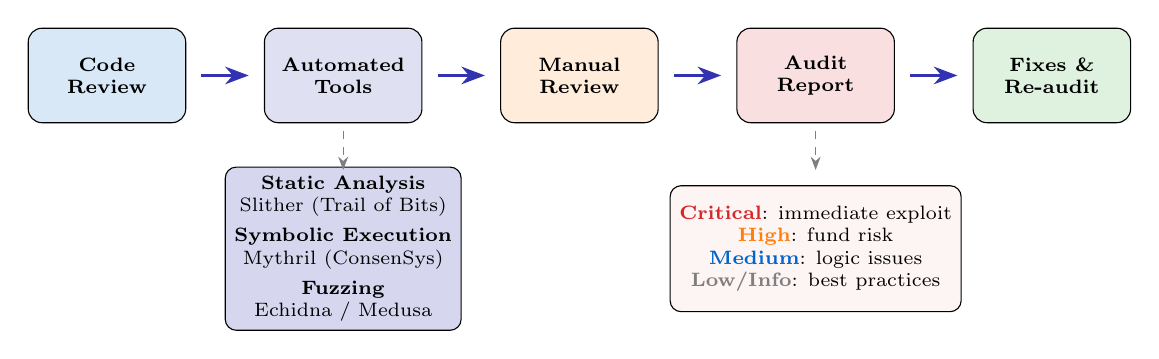
\begin{tikzpicture}[
  auditbox/.style={draw,rounded corners=5pt,minimum width=2cm,minimum height=1.2cm,
    font=\scriptsize\bfseries,align=center},
  arr/.style={-{Stealth[length=3mm]},thick,mlpurple}
]
  % Audit process flow
  \node[auditbox,fill=mlblue!15] (code) at (0,0) {Code\\Review};
  \node[auditbox,fill=mlpurple!15] (auto) at (3,0) {Automated\\Tools};
  \node[auditbox,fill=mlorange!15] (manual) at (6,0) {Manual\\Review};
  \node[auditbox,fill=mlred!15] (report) at (9,0) {Audit\\Report};
  \node[auditbox,fill=mlgreen!15] (fix) at (12,0) {Fixes \&\\Re-audit};

  \draw[arr] (1.2,0) -- (1.8,0);
  \draw[arr] (4.2,0) -- (4.8,0);
  \draw[arr] (7.2,0) -- (7.8,0);
  \draw[arr] (10.2,0) -- (10.8,0);

  % Tools
  \node[draw,rounded corners=4pt,fill=mllavender4,font=\scriptsize,align=center,
    minimum width=2.8cm,minimum height=1.6cm] (tools) at (3,-2.2) {
    \textbf{Static Analysis}\\
    Slither (Trail of Bits)\\[1mm]
    \textbf{Symbolic Execution}\\
    Mythril (ConsenSys)\\[1mm]
    \textbf{Fuzzing}\\
    Echidna / Medusa
  };
  \draw[-{Stealth},mlgray,dashed] (3,-0.7) -- (3,-1.2);

  % Report details
  \node[draw,rounded corners=4pt,fill=mlred!5,font=\scriptsize,align=center,
    minimum width=3cm,minimum height=1.6cm] (rep) at (9,-2.2) {
    \textcolor{mlred}{\textbf{Critical}}: immediate exploit\\
    \textcolor{mlorange}{\textbf{High}}: fund risk\\
    \textcolor{mlblue}{\textbf{Medium}}: logic issues\\
    \textcolor{mlgray}{\textbf{Low/Info}}: best practices
  };
  \draw[-{Stealth},mlgray,dashed] (9,-0.7) -- (9,-1.2);
\end{tikzpicture}
\end{center}
\vspace{2mm}
\begin{columns}
\column{0.48\textwidth}
\begin{block}{Audit Economics}
\small
\begin{tabular}{@{}lr@{}}
\toprule
\textbf{Scope} & \textbf{Typical Cost} \\
\midrule
Simple token & \$5K--\$15K \\
DeFi protocol & \$50K--\$200K \\
Complex protocol & \$200K--\$500K \\
\bottomrule
\end{tabular}\\[2mm]
\textbf{Timeline}: 1--8 weeks depending on complexity
\end{block}
\column{0.48\textwidth}
\begin{alertblock}{Audits Are Necessary But Not Sufficient}
\small An audit is a \emph{point-in-time} review. It does not guarantee zero bugs. Combine with:
\begin{itemize}\small
  \item Bug bounty programs (Immunefi)
  \item Formal verification
  \item Continuous monitoring
  \item Upgrade timelocks
\end{itemize}
\end{alertblock}
\end{columns}
\bottomnote{Top audit firms: Trail of Bits, OpenZeppelin, Consensys Diligence, Spearbit, Cyfrin -- demand exceeds supply}
\end{frame}

%--- FRAME 53: Ethereum by the Numbers ---
\begin{frame}{Ethereum by the Numbers}
\begin{center}
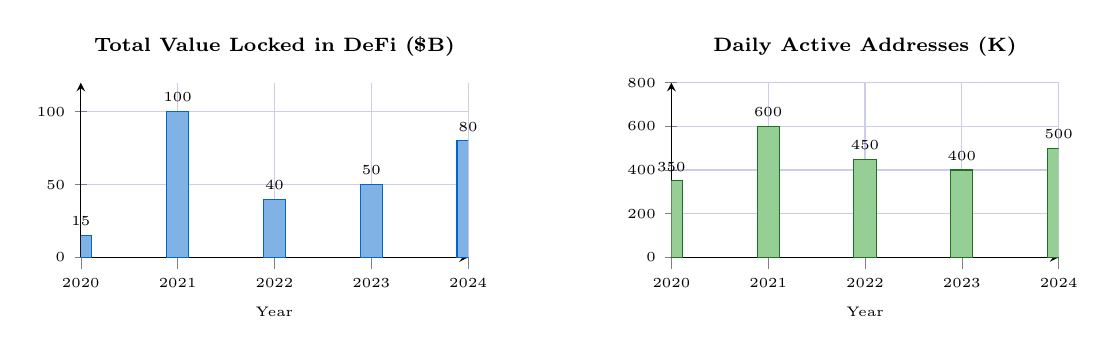
\begin{tikzpicture}
  % TVL chart
  \begin{axis}[
    name=tvl,
    at={(0,0)},
    width=6.5cm, height=3.8cm,
    title={\scriptsize\bfseries Total Value Locked in DeFi (\$B)},
    title style={font=\scriptsize\bfseries},
    xlabel={Year},
    xlabel style={font=\tiny},
    ylabel style={font=\tiny},
    tick label style={font=\tiny},
    xtick={2020,2021,2022,2023,2024},
    xticklabels={2020,2021,2022,2023,2024},
    ymin=0, ymax=120,
    grid=major,
    grid style={mllavender3},
    axis lines=left,
    ybar,
    bar width=8pt,
    nodes near coords={\tiny\pgfmathprintnumber\pgfplotspointmeta},
    every node near coord/.append style={font=\tiny,above}
  ]
  \addplot[fill=mlblue!50,draw=mlblue] coordinates {
    (2020,15) (2021,100) (2022,40) (2023,50) (2024,80)
  };
  \end{axis}

  % Daily active addresses
  \begin{axis}[
    name=daa,
    at={(7.5cm,0)},
    width=6.5cm, height=3.8cm,
    title={\scriptsize\bfseries Daily Active Addresses (K)},
    title style={font=\scriptsize\bfseries},
    xlabel={Year},
    xlabel style={font=\tiny},
    ylabel style={font=\tiny},
    tick label style={font=\tiny},
    xtick={2020,2021,2022,2023,2024},
    xticklabels={2020,2021,2022,2023,2024},
    ymin=0, ymax=800,
    grid=major,
    grid style={mllavender3},
    axis lines=left,
    ybar,
    bar width=8pt,
    nodes near coords={\tiny\pgfmathprintnumber\pgfplotspointmeta},
    every node near coord/.append style={font=\tiny,above}
  ]
  \addplot[fill=mlgreen!50,draw=mlgreen!70!black] coordinates {
    (2020,350) (2021,600) (2022,450) (2023,400) (2024,500)
  };
  \end{axis}
\end{tikzpicture}
\end{center}
\vspace{1mm}
\begin{columns}
\column{0.48\textwidth}
\begin{block}{ETH Burned Since EIP-1559}
\colorbox{mlorange!10}{\parbox{0.92\linewidth}{\small
\begin{itemize}
  \item Over \textbf{4M+ ETH} burned ($>$\$8B+ at peak)
  \item Net deflationary during high activity
  \item ``Ultrasound money'' narrative
  \item Burn rate: 1--5 ETH/min average
\end{itemize}
}}
\end{block}
\column{0.48\textwidth}
\begin{block}{Validator Ecosystem}
\colorbox{mlpurple!10}{\parbox{0.92\linewidth}{\small
\begin{itemize}
  \item \textbf{900K+} active validators
  \item 32 ETH minimum stake
  \item $\sim$28M ETH staked ($\sim$23\% supply)
  \item Lido, Coinbase, Rocket Pool dominate
\end{itemize}
}}
\end{block}
\end{columns}
\bottomnote{Ethereum processes $\sim$1M transactions/day on L1, with L2s adding another $\sim$5M+/day -- the ecosystem continues to grow}
\end{frame}

%--- FRAME 54: Career Paths in Ethereum ---
\begin{frame}{Career Paths in Ethereum}
\begin{center}
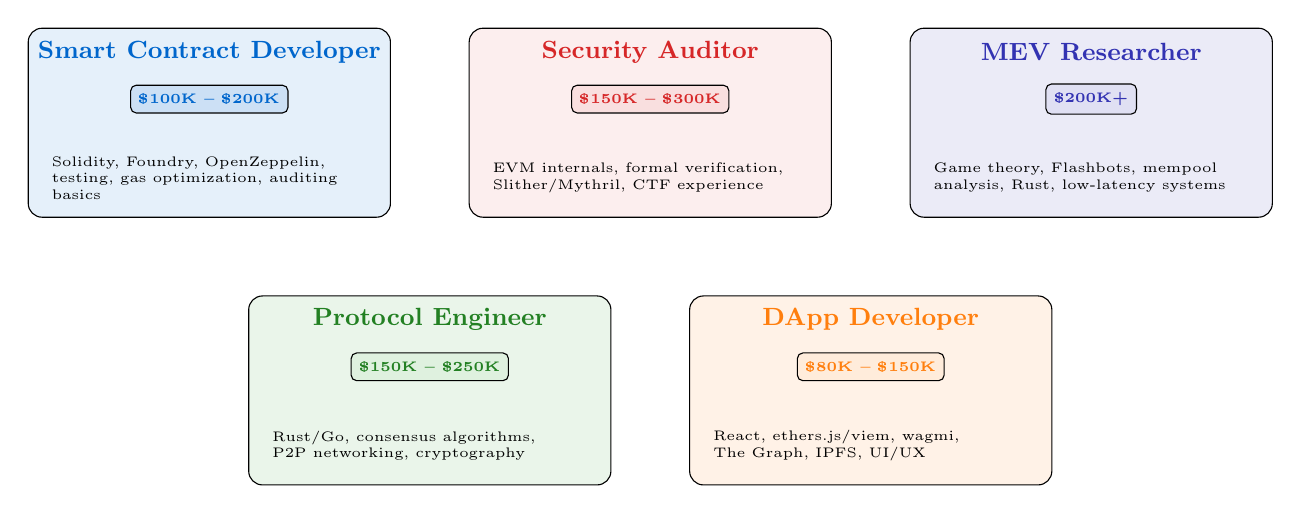
\begin{tikzpicture}[
  career/.style={draw,rounded corners=5pt,minimum width=4.6cm,minimum height=2.4cm,
    font=\small,align=center},
  skill/.style={font=\tiny,align=left,text width=4cm},
  salary/.style={draw,rounded corners=2pt,font=\tiny\bfseries,inner sep=3pt}
]
  % Row 1
  \node[career,fill=mlblue!10] (c1) at (0,2.2) {};
  \node[font=\small\bfseries,mlblue] at (0,3.1) {Smart Contract Developer};
  \node[salary,fill=mlblue!20,text=mlblue] at (0,2.5) {\$100K -- \$200K};
  \node[skill] at (0,1.5) {Solidity, Foundry, OpenZeppelin,\\testing, gas optimization, auditing basics};

  \node[career,fill=mlred!8] (c2) at (5.6,2.2) {};
  \node[font=\small\bfseries,mlred] at (5.6,3.1) {Security Auditor};
  \node[salary,fill=mlred!15,text=mlred] at (5.6,2.5) {\$150K -- \$300K};
  \node[skill] at (5.6,1.5) {EVM internals, formal verification,\\Slither/Mythril, CTF experience};

  \node[career,fill=mlpurple!10] (c3) at (11.2,2.2) {};
  \node[font=\small\bfseries,mlpurple] at (11.2,3.1) {MEV Researcher};
  \node[salary,fill=mlpurple!15,text=mlpurple] at (11.2,2.5) {\$200K+};
  \node[skill] at (11.2,1.5) {Game theory, Flashbots, mempool\\analysis, Rust, low-latency systems};

  % Row 2
  \node[career,fill=mlgreen!10] (c4) at (2.8,-1.2) {};
  \node[font=\small\bfseries,mlgreen!80!black] at (2.8,-0.3) {Protocol Engineer};
  \node[salary,fill=mlgreen!15,text=mlgreen!80!black] at (2.8,-0.9) {\$150K -- \$250K};
  \node[skill] at (2.8,-1.9) {Rust/Go, consensus algorithms,\\P2P networking, cryptography};

  \node[career,fill=mlorange!10] (c5) at (8.4,-1.2) {};
  \node[font=\small\bfseries,mlorange] at (8.4,-0.3) {DApp Developer};
  \node[salary,fill=mlorange!15,text=mlorange] at (8.4,-0.9) {\$80K -- \$150K};
  \node[skill] at (8.4,-1.9) {React, ethers.js/viem, wagmi,\\The Graph, IPFS, UI/UX};
\end{tikzpicture}
\end{center}
\vspace{1mm}
\begin{alertblock}{Getting Started}
\small \textbf{Path 1}: CryptoZombies $\to$ Foundry $\to$ CTFs (Ethernaut, Damn Vulnerable DeFi) $\to$ build projects $\to$ contribute to protocols. \textbf{Path 2}: Web2 dev $\to$ learn ethers.js $\to$ build DApps $\to$ learn Solidity $\to$ full-stack Web3.
\end{alertblock}
\bottomnote{Web3 salaries remain 20--50\% above Web2 equivalents -- the talent shortage is real and growing}
\end{frame}

%--- FRAME 55: Course Takeaways ---
\begin{frame}{Course Takeaways}
\begin{columns}
\column{0.52\textwidth}
\begin{block}{Five Key Principles}
\begin{itemize}\small
  \item[$\checkmark$] \textbf{Ethereum = programmable blockchain} with a Turing-complete EVM enabling arbitrary on-chain logic
  \item[$\checkmark$] \textbf{Gas prevents abuse} and pays validators for computation -- EIP-1559 makes fees predictable
  \item[$\checkmark$] \textbf{Solidity enables complex on-chain logic} with types, storage, events, and design patterns
  \item[$\checkmark$] \textbf{Security is paramount} -- audit everything, use established patterns, test exhaustively
  \item[$\checkmark$] \textbf{The ecosystem is composable} (money legos) -- protocols build on protocols permissionlessly
\end{itemize}
\end{block}
\vspace{1mm}
\begin{alertblock}{Remember}
\small Smart contracts are \textbf{immutable} and handle \textbf{real value}. Every line of code is a potential attack surface. Think like an attacker, build like a defender.
\end{alertblock}
\column{0.44\textwidth}
\begin{center}
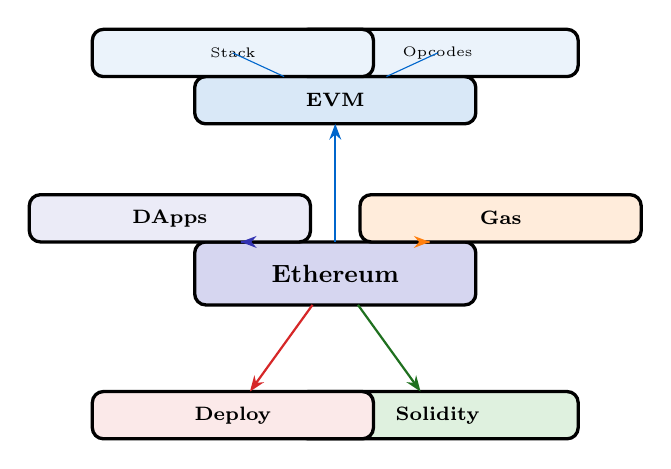
\begin{tikzpicture}[
  mindmap,
  every node/.style={draw,rounded corners=4pt,font=\scriptsize\bfseries,align=center,
    minimum width=1.4cm,minimum height=0.6cm},
  level 1/.style={sibling angle=72,level distance=2.2cm},
  arr/.style={-{Stealth[length=2mm]},thick}
]
  % Central node
  \node[fill=mlpurple!20,font=\small\bfseries,minimum width=2cm,minimum height=0.8cm] (eth) at (0,0) {Ethereum};

  % Branches
  \node[fill=mlblue!15] (evm) at (0,2.2) {EVM};
  \node[fill=mlorange!15] (gas) at (2.1,0.7) {Gas};
  \node[fill=mlgreen!15] (sol) at (1.3,-1.8) {Solidity};
  \node[fill=mlred!10] (dep) at (-1.3,-1.8) {Deploy};
  \node[fill=mlpurple!10] (dapp) at (-2.1,0.7) {DApps};

  \draw[arr,mlblue] (eth) -- (evm);
  \draw[arr,mlorange] (eth) -- (gas);
  \draw[arr,mlgreen!70!black] (eth) -- (sol);
  \draw[arr,mlred] (eth) -- (dep);
  \draw[arr,mlpurple] (eth) -- (dapp);

  % Sub-branches
  \node[fill=mlblue!8,font=\tiny,minimum width=1cm] at (1.3,2.8) {Opcodes};
  \node[fill=mlblue!8,font=\tiny,minimum width=1cm] at (-1.3,2.8) {Stack};
  \draw[mlblue,thin] (evm) -- (1.3,2.8);
  \draw[mlblue,thin] (evm) -- (-1.3,2.8);
\end{tikzpicture}
\end{center}
\end{columns}
\bottomnote{Next lecture: Build your own ERC-20 token!}
\end{frame}

\end{document}
